\documentclass[12pt,a4paper, twoside, openright]{report}
\usepackage[italian]{babel}
\usepackage[utf8]{inputenc}
\usepackage[T1]{fontenc}

\usepackage{amsmath}
\usepackage{amssymb}
\usepackage{amsfonts}
\usepackage{graphicx}
\usepackage{subcaption}
\usepackage{booktabs}
\usepackage{float}
\usepackage{siunitx}
\usepackage{hyperref}
\usepackage{cleveref}

\usepackage[nottoc]{tocbibind}

\usepackage{listings}
\usepackage{xcolor}

\lstset{
    language=C++,
    numbers=left,
    numbersep=10pt,
    basicstyle=\ttfamily\small,
    keywordstyle=\color{blue}\bfseries,
    commentstyle=\color{green!60!black},
    stringstyle=\color{red},
    breaklines=true,
    frame=single,
    showstringspaces=false,
    tabsize=2
}

\title{Pianificazione e ottimizzazione di traiettorie per la robotica collaborativa}
\date{\today}


\begin{document}

\maketitle

\pagenumbering{roman}

\chapter*{Sommario}
\addcontentsline{toc}{chapter}{Sommario}

Il presente lavoro di tesi si colloca nell'ambito della  robotica collaborativa (Human-Robot Collaboration, HRC) e presenta lo sviluppo di un'architettura software di controllo allo scopo di garantire la sicurezza durante le attività lavorative. L'obiettivo del percorso è l'implementazione in C++ di un algoritmo di arresto ottimo, basato sull'ottimizzazione del tempo di arresto e sul controllo d'impedenza. Questo approccio viene in seguito confrontato con una metodologia basata su forze repulsive e sul controllo d'ammettenza.

Per gestire le zone di sicurezza, il manipolatore robotico e l'operatore umano vengono modellati come una serie di capsule geometriche (Sphere-Swept Lines, SSL) con dimensioni dinamiche, variabili in base allo stato cinematico (velocità e accelerazioni) del robot. Questa modellazione semplifica notevolmente il calcolo delle distanze relative, garantendo la gestione delle interazioni in tempo reale.

La validzione sperimentale è stata condotta su un cobot Franka Emika Panda a 7 gradi di libertà. Il tracciamento dell'operatore nello spazio tridimensionale è affidato a una telecamera di profondità Intel RealSense D435 accoppiata all'algoritmo YOLOv8 per la stima della posa. Lo scambio di dati a bassa latenza tra il nodo di visione e il nodo di controllo è realizzato tramite la libreria di messaggistica ZeroMQ.

Infine, le due startegie di controllo vengono confrontate sulla base di metriche prestazionali concrete: tempo totale di esecuzione ($T_{TASK}$), tempo di inattività del robot ($R_{IDLE}$), tempo di attività concorrente nello spazio di lavoro ($C_{ACT-WS}$) e numero di arresti del robot ($R_{STOPS}$).
 
\tableofcontents

\listoffigures

\clearpage
\pagenumbering{arabic}

\chapter{Introduzione}
\section{Collaborazione uomo-robot}

La robotica industriale ha assunto un ruolo sempre più rilevante nei moderni processi produttivi, grazie alla possibilità di automatizzare attività ripetitive, incrementare la produttività e garantire elevati livelli di precisione e ripetibilità. Tradizionalmente, l'impiego di robot industriali è stato caratterizzato dalla separazione fisica tra l'area di lavoro dell'operatore e quella del robot, mediante l'utilizzo di barriere, recinzioni o altri dispositivi volti a impedire l'accesso dell'uomo alla zona operativa durante il movimento del robot.
Questo approccio permette di ridurre il rischio di interazione accidentale, separando nettamente le attività svolte dall'uomo e quelle affidate al sistema robotico. Tale separazione, tuttavia, può risultare poco conveniente in applicazioni nelle quali le capacità del lavoratore e quelle del robot possono essere integrate per ottenere un processo più efficiente e flessibile.

Da questa esigenza nasce il concetto di collaborazione uomo-robot, nel quale l'operatore umano e la macchina robotica operano all'interno di uno spazio condiviso, come schematizzato in Figura \ref{fig:collaborazione}, e possono contribuire simultaneamente alla realizzazione di uno stesso compito \cite{BARATTA20231887}. In questo contesto, il robot non viene più considerato come un sistema autonomo e separato dall'operatore, ma come uno strumento in grado di interagire con esso e di supportarne le attività. La condivisione dello spazio di lavoro permette quindi di combinare le caratteristiche complementari dell'uomo e del robot, con l'obiettivo di ottenere sistemi produttivi più flessibili e adattabili rispetto alle soluzioni di automazione tradizionali.

\begin{figure}[htbp]
    \centering
    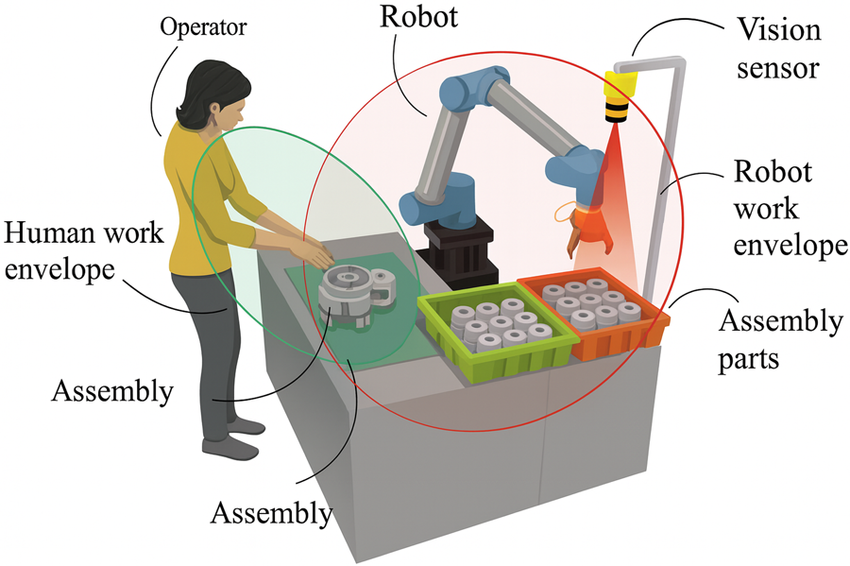
\includegraphics[width=0.8\linewidth]{figure_tesi/Application-of-cobots-in-the-manufacturing-process.png}
    \caption{Rappresentazione schematica di una cella di lavoro collaborativa. Viene evidenziata la sovrapposizione tra il volume operativo dell'operatore (\textit{Human work envelope}) e l'area di lavoro del robot (\textit{Robot work envelope}).}
    \label{fig:collaborazione}
\end{figure}

Le applicazioni della collaborazione uomo-robot sono principalmente legate a situazioni nelle quali le capacità dell'operatore e quelle del robot risultano complementari \cite{Montini2024}. Il robot può, ad esempio, occuparsi di attività caratterizzate da elevata ripetibilità, precisione o movimentazione di carichi, mentre l'operatore può intervenire nelle operazioni che richiedono capacità decisionali, adattamento a condizioni variabili o manipolazioni più complesse. Questa suddivisione delle attività permette di sfruttare i vantaggi dell'automazione mantenendo, allo stesso tempo, la flessibilità e la capacità di adattamento proprie dell'operatore umano.

La collaborazione diretta tra uomo e robot può quindi trovare applicazione in diversi processi industriali, tra cui assemblaggio, movimentazione, manipolazione e attività di supporto all'operatore. In questi scenari, la possibilità di lavorare all'interno dello stesso spazio consente di ridurre la necessità di separare fisicamente le due attività e di progettare processi nei quali uomo e robot possano intervenire in maniera complementare sullo stesso task.

La condivisione dello spazio di lavoro introduce tuttavia una problematica fondamentale: la necessità di garantire condizioni di sicurezza durante l'interazione. A differenza delle applicazioni tradizionali, nelle quali la presenza dell'operatore nella zona di movimento del robot viene impedita, nei sistemi collaborativi la presenza umana deve essere considerata come una condizione normale di funzionamento. La gestione della sicurezza assume quindi un ruolo centrale nella progettazione di questi sistemi e rappresenta uno degli aspetti fondamentali per consentire una collaborazione efficace tra uomo e robot.

\section{Sicurezza nella collaborazione uomo-robot}

La possibilità di condividere lo spazio di lavoro tra operatore umano e robot introduce la necessità di adottare specifiche strategie volte a garantire la sicurezza dell'interazione \cite{Li2024}. Il rischio associato alla collaborazione dipende infatti da diversi fattori, tra cui la geometria del robot, la velocità di movimento, le caratteristiche dell'ambiente di lavoro e la posizione dell'operatore rispetto al sistema robotico.

Un primo elemento che può contribuire alla riduzione delle conseguenze di un eventuale contatto è rappresentato dalla progettazione del robot. La geometria e i materiali utilizzati per la realizzazione dei componenti che possono entrare in contatto con l'operatore possono infatti influenzare le conseguenze di una collisione. In particolare, l'impiego di superfici arrotondate e l'assenza di spigoli vivi permettono di ridurre la possibilità che un eventuale contatto provochi lesioni all'operatore. Sebbene questi accorgimenti contribuiscano alla sicurezza del sistema, essi non sono sufficienti a garantire autonomamente condizioni di sicurezza durante l'interazione.

La sicurezza dei sistemi robotici collaborativi è pertanto regolamentata da specifici standard internazionali, che definiscono principi e requisiti per la progettazione e la valutazione delle applicazioni di collaborazione uomo-robot \cite{ISO15066}. Tra gli aspetti considerati rientrano anche le condizioni che devono essere rispettate affinché l'operatore possa condividere lo spazio di lavoro con il robot in condizioni di sicurezza.

Un aspetto particolarmente rilevante è rappresentato dalla distanza tra l'operatore e il robot. Durante il movimento, infatti, è necessario che il sistema sia in grado di rilevare una situazione potenzialmente pericolosa con sufficiente anticipo da permettere l'adozione di un'azione correttiva prima che si verifichi un contatto. La distanza necessaria non può quindi essere considerata come un valore fisso, ma deve essere valutata tenendo conto della dinamica del sistema e, in particolare, della velocità del robot e dell'operatore e dei tempi necessari affinché il sistema possa reagire alla situazione di rischio \cite{Marvel2017}.

Un approccio alla gestione di questo problema è rappresentato dallo \textit{Speed and Separation Monitoring} (SSM), nel quale la distanza tra l'operatore e il robot viene monitorata durante l'esecuzione del task. Con riferimento alla Figura \ref{fig:SSM}, quando la separazione tra i due è tale da non garantire più le condizioni di sicurezza, il sistema può intervenire modificando il comportamento del robot, ad esempio riducendone la velocità (zona gialla) o arrestandone il movimento (zona rossa). La distanza necessaria per garantire la sicurezza dipende quindi dalle condizioni di funzionamento del sistema e deve essere valutata considerando anche il tempo necessario affinché il robot possa effettuare l'azione prevista.

\begin{figure}
    \centering
    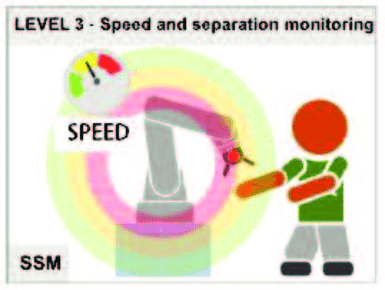
\includegraphics[width=0.5\linewidth]{figure_tesi/Speed-and-separation-monitoringVillani-et-al-2018.png}
    \caption{Rappresentazione schematica del principio di Speed and Separation Monitoring (SSM).}
    \label{fig:SSM}
\end{figure}

Nell'ambito dello SSM sono state sviluppate diverse strategie finalizzate a migliorare il compromesso tra sicurezza e continuità operativa. Un arresto del robot ogni volta che l'operatore si avvicina alla zona di lavoro permette di adottare un comportamento conservativo, ma può comportare frequenti interruzioni dell'attività e conseguenti riduzioni della produttività. Per questo motivo, sono state studiate strategie che permettono di adattare dinamicamente le condizioni di sicurezza in funzione del movimento del robot e dell'operatore. In particolare, Scalera et al. \cite{Scalera2022} propongono una strategia basata sullo scaling online delle zone di sicurezza dinamiche, con l'obiettivo di migliorare la fluidità e la produttività della collaborazione mantenendo le condizioni di sicurezza.

Il presente lavoro si inserisce in questo contesto e si concentra sul confronto tra due differenti strategie software per la gestione di una possibile situazione di collisione. Le due procedure utilizzano le informazioni relative alla posizione dell'operatore e al movimento del robot per valutare le condizioni di sicurezza, ma adottano strategie differenti per la gestione del movimento. La prima procedura prevede l'arresto del robot quando viene prevista una possibile collisione, mentre la seconda modifica il movimento del robot con l'obiettivo di mantenere una distanza di sicurezza dall'operatore senza ricorrere necessariamente all'arresto completo.

\section{Obiettivo della tesi}

L'obiettivo del presente lavoro di tesi è quello di sviluppare e analizzare due strategie di controllo per la collaborazione sicura uomo-robot, entrambe basate sull'utilizzo della visione artificiale per il rilevamento della presenza e della posizione dell'operatore all'interno dello spazio di lavoro del robot.

La prima strategia, arresto forzato, deriva dagli studi di Scalera et al. \cite{Scalera2022}, che hanno analizzato l'impiego di capsule di ingombro dinamiche, chiamate \textit{Sphere Swept Lines} o SSL, secondo il paradigma di \textit{Speed and Separation Monitoring} o SSM. In particolare viene calcolato il tempo minimo di arresto del robot in funzioni di vari vincoli del robot. 
La seconda strategia estende il primo approccio introducendo una tecnica di modifica del movimento del robot basato su un controllo di ammettenza \cite{Qyrani2026}. In questo modo il robot mantiene una distanza di sicurezza modificando la propria traiettoria, evitando se possibile l'arresto completo del robot.
Il confronto viene effettuato attraverso le seguenti metriche:
\begin{itemize}
    \item durata complessiva di esecuzione del task
    \item tempo durante il quale il robot è fermo
    \item numero di arresti
    \item tempo durante il quale operatore e robot risultano contemporaneamente attivi all'interno dello spazio di lavoro
\end{itemize}

Lo studio mira quindi a determinare le caratteristiche e le prestazioni delle due strategie e ad evidenziarne vantaggi e limiti in relazione all'impiego in scenari di collaborazione uomo-robot.

\section{Struttura della tesi}

La tesi è organizzata in cinque capitoli che descrivono il processo di riconoscimento del problema, implementazione di una soluzione e confronto tra i due approcci software.

Il primo capitolo introduce il contesto della collaborazione uomo-robot, descrivendo le principali problematiche legate alla sicurezza dell'interazione e presentando gli obiettivi del lavoro.

Nel secondo capitolo vengono descritti i due approcci proposti per la gestione della sicurezza. Per ciascuna procedura vengono illustrati il principio d funzionamento, le grandezze considerate e la strategia adottata per la gestione del movimento del robot.

Il terzo capitolo è dedicato all'implementazione sperimentale. Vengono presentati il sistema robotico utilizzato, l'ambiente di sviluppo, l'implementazione delle due procedure e la configurazione degli esperimenti. Vengono inoltre definite le metriche utilizzate per il confronto e il protocollo sperimentale adottato.

Nel quarto capitolo vengono presentati e discussi i risultati ottenuti durante la fase sperimentale. Le due procedure vengono confrontate sulla base delle metriche definite, analizzandone il comportamento in termini di sicurezza, continuità operativa ed efficienza nell'esecuzione del task.

Il quinto capitolo, infine, riassume i principali risultati del lavoro e presenta le conclusioni dello studio, evidenziando vantaggi e limiti delle due stratege utilizzate e indicando possibili sviluppi futuri.

\chapter{Approcci considerati}

\section{Rappresentazione geometrica del sistema}
Prima di definire le strategie di gestione della sicurezza, è necessario introdurre una rappresentazione geometrica del robot e dell'operatore che possa essere impiegata per effettuare le verifiche di prossimità in tempo reale. La geometria reale di un manipolatore e del corpo umano è infatti complessa e una sua modellazione dettagliata risulterebbe computazionalmente troppo onerosa per i calcoli da eseguire continuamente durante il movimento. Per questo motivo, entrambi vengono approssimati mediante volumi geometrici semplificati (primitive geometriche).

\subsection{Sphere Swept Lines (SSL)}

Una delle rappresentazioni più diffuse per questo scopo è costituita dalle \textit{Sphere Swept Lines} (SSL), le quali permettono di approssimare la geometria di un corpo tramite l'unione di un segmento e di una sfera. Nel caso di un segmento di estremi $P_0$ e $P_1$, la SSL corrispondente è definita formalmente come la somma di Minkowski tra il segmento $\overline{P_0P_1}$ e una sfera di raggio $r$ \cite{larsen1999fast}.

In generale, dati due insiemi $A$ e $B$ nello spazio euclideo, la loro somma di Minkowski è definita come:
\begin{equation}
    A+B = \{a+b \mid a\in A,\; b\in B\}.
\end{equation}

Nel caso specifico delle SSL, la somma di Minkowski tra il segmento e la sfera genera un solido a forma di capsula, interpretabile come il luogo dei punti nello spazio aventi distanza minore o uguale a $r$ dal segmento $\overline{P_0P_1}$.

\begin{figure}[htbp]
    \centering
    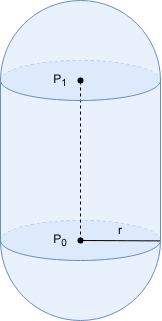
\includegraphics[width=0.2\linewidth]{figure_tesi/SSL.png}
    \caption{Rappresentazione geometrica di una Sphere Swept Line (SSL).}
    \label{fig:SSL}
\end{figure}

L'impiego delle SSL consente quindi di sostituire una geometrie tridimensionali articolate con un insieme contenuto di primitive, semplificando notevolemnte il calcolo algebrico delle distanze minime e l'individuazione di eventuali intersezioni tra robot e operatore.

\subsection{Modellazione del robot e dell'operatore}

Nel presente lavoro, il robot utilizzato per le prove sperimentali è un manipolatore Franka Emika Panda a sette gradi di libertà. Ai fini della valutazione della distanza dall'operatore, la struttura del robot viene approssimata tramite un insieme di quattro SSL (capsule), associate rispettivamente alle coppe di giunti principali: base-1, 2-3, 4-5, 6-flangia. In figura \ref{fig:robot_modellazione} si può osservare 

I segmenti delle capsule vengono definiti in tempo reale a partire dalla cinematica diretta del robot, quindi dalle posizioni dei giunti, mentre il raggio $r$ di ciascuna SSL viene opportunamente dimensionato in modo da racchiudere interamente il volume del braccio robotico nel tratto corrispondente. L'aggiornamento continuo della posizione dei giunti durante il moto permette di ricalcolare istante per istante la posa delle SSL, consentendo quindi di effettuare le verifiche di sicurezza in tempo reale.

\begin{figure}[htbp]
    \centering
    \begin{subfigure}[b]{1\textwidth}
        \centering
        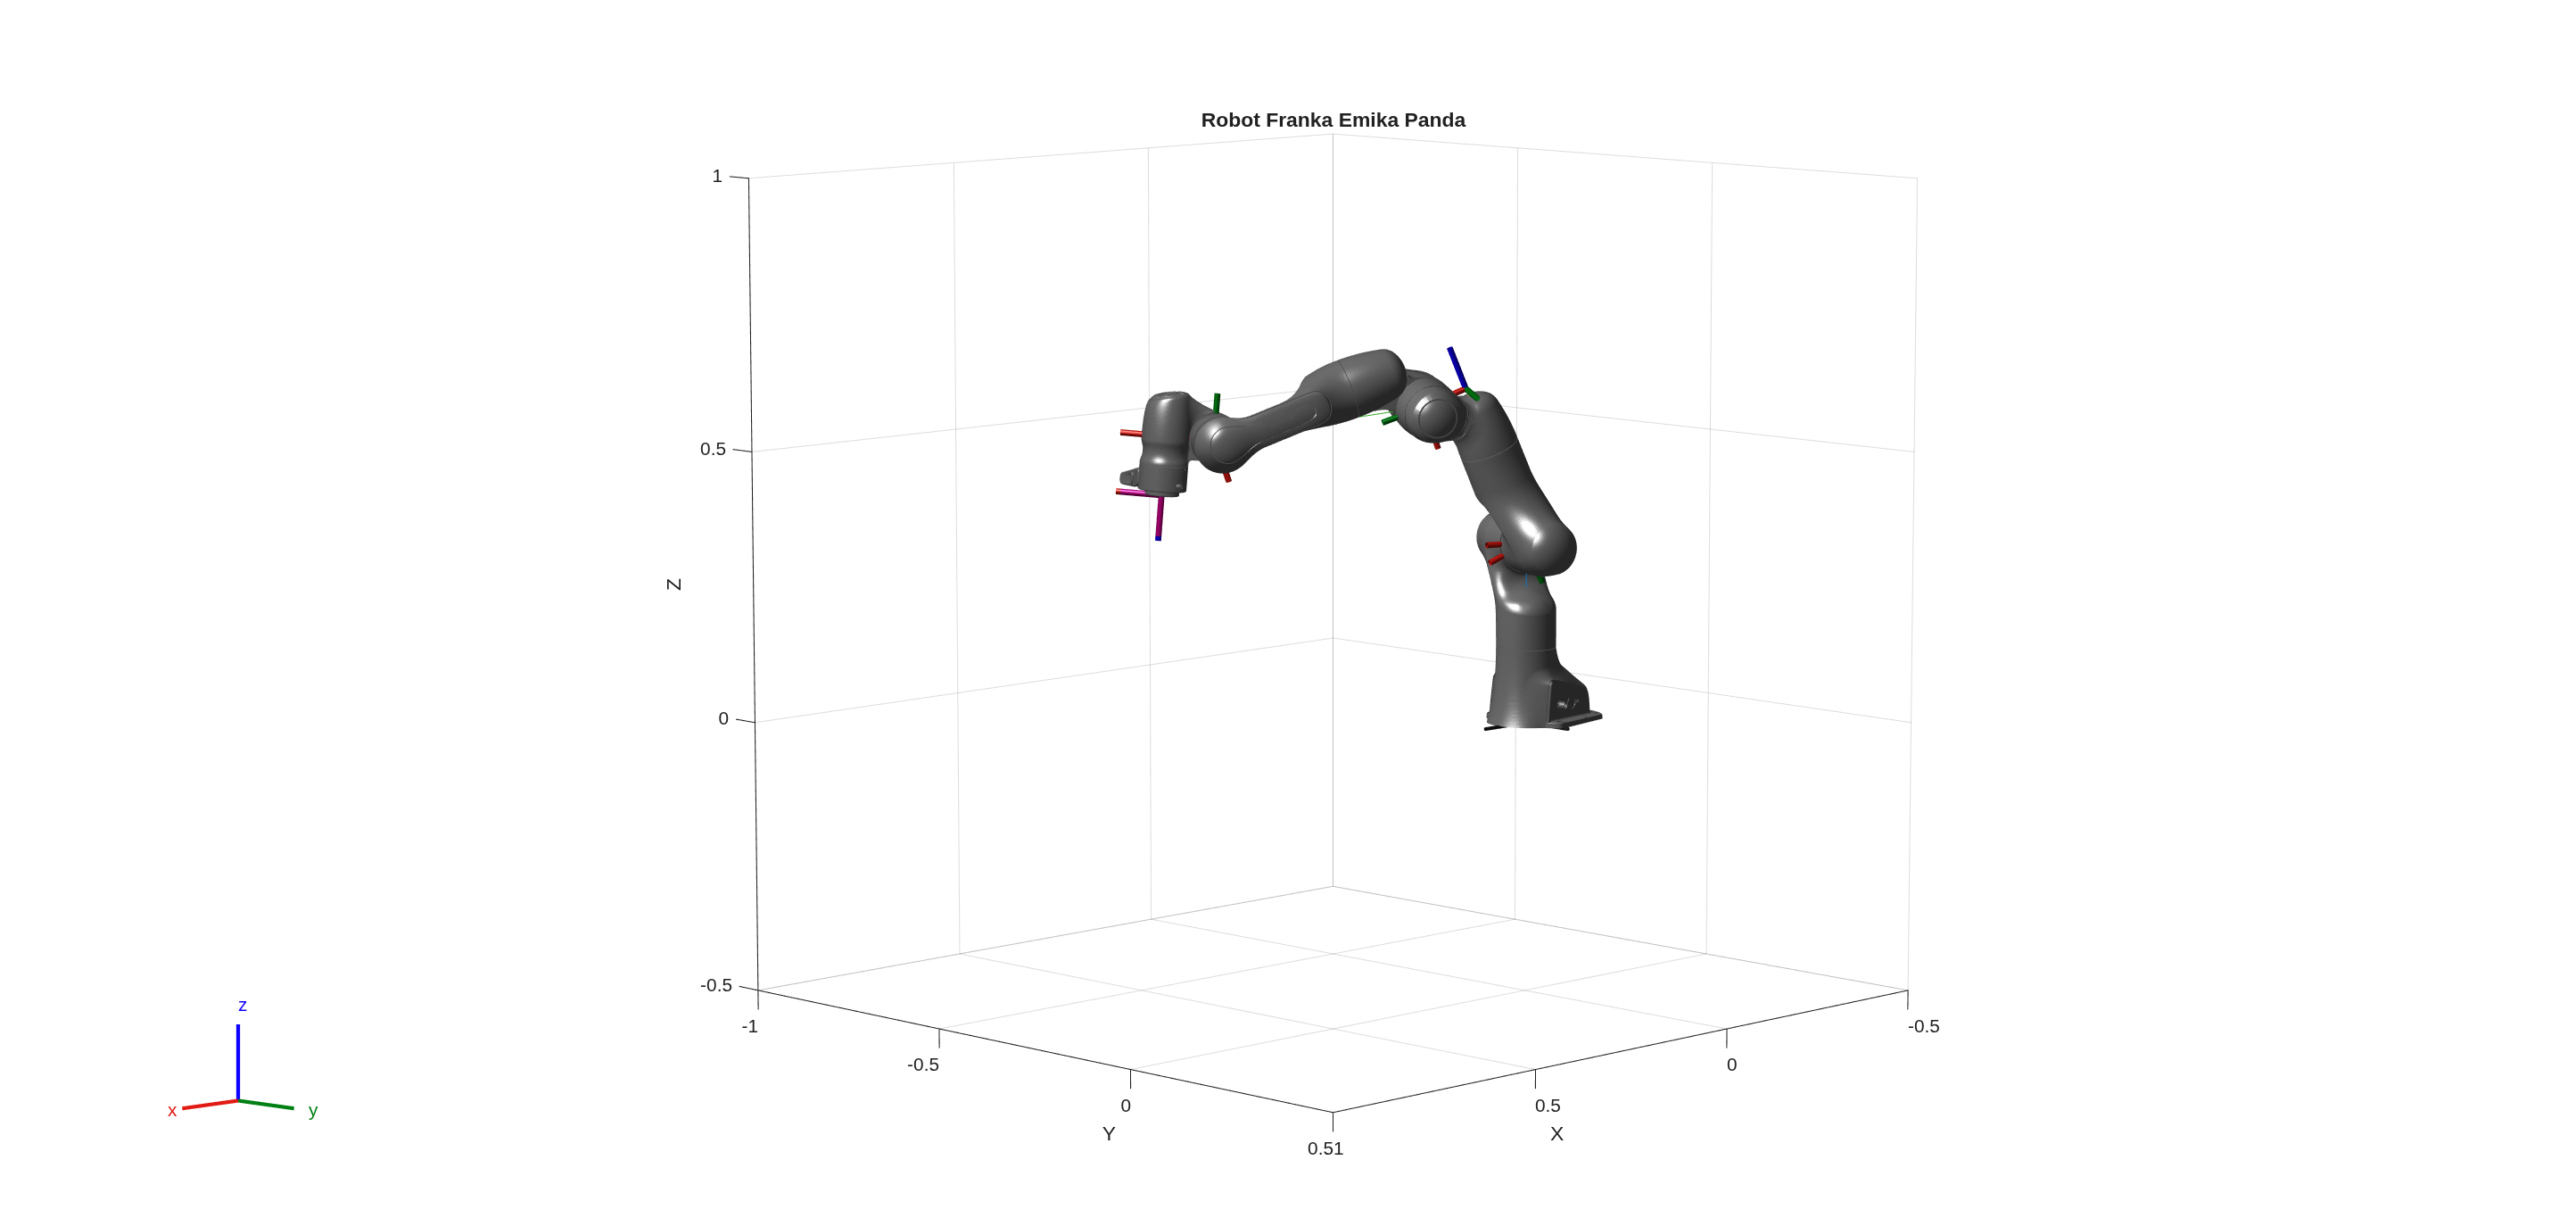
\includegraphics[width=\textwidth]{figure_tesi/robot.png}
        \caption{Robot Panda nella configurazione iniziale}
        \label{fig:robot}
    \end{subfigure}
    \hfill
    \begin{subfigure}[b]{1\textwidth}
        \centering
        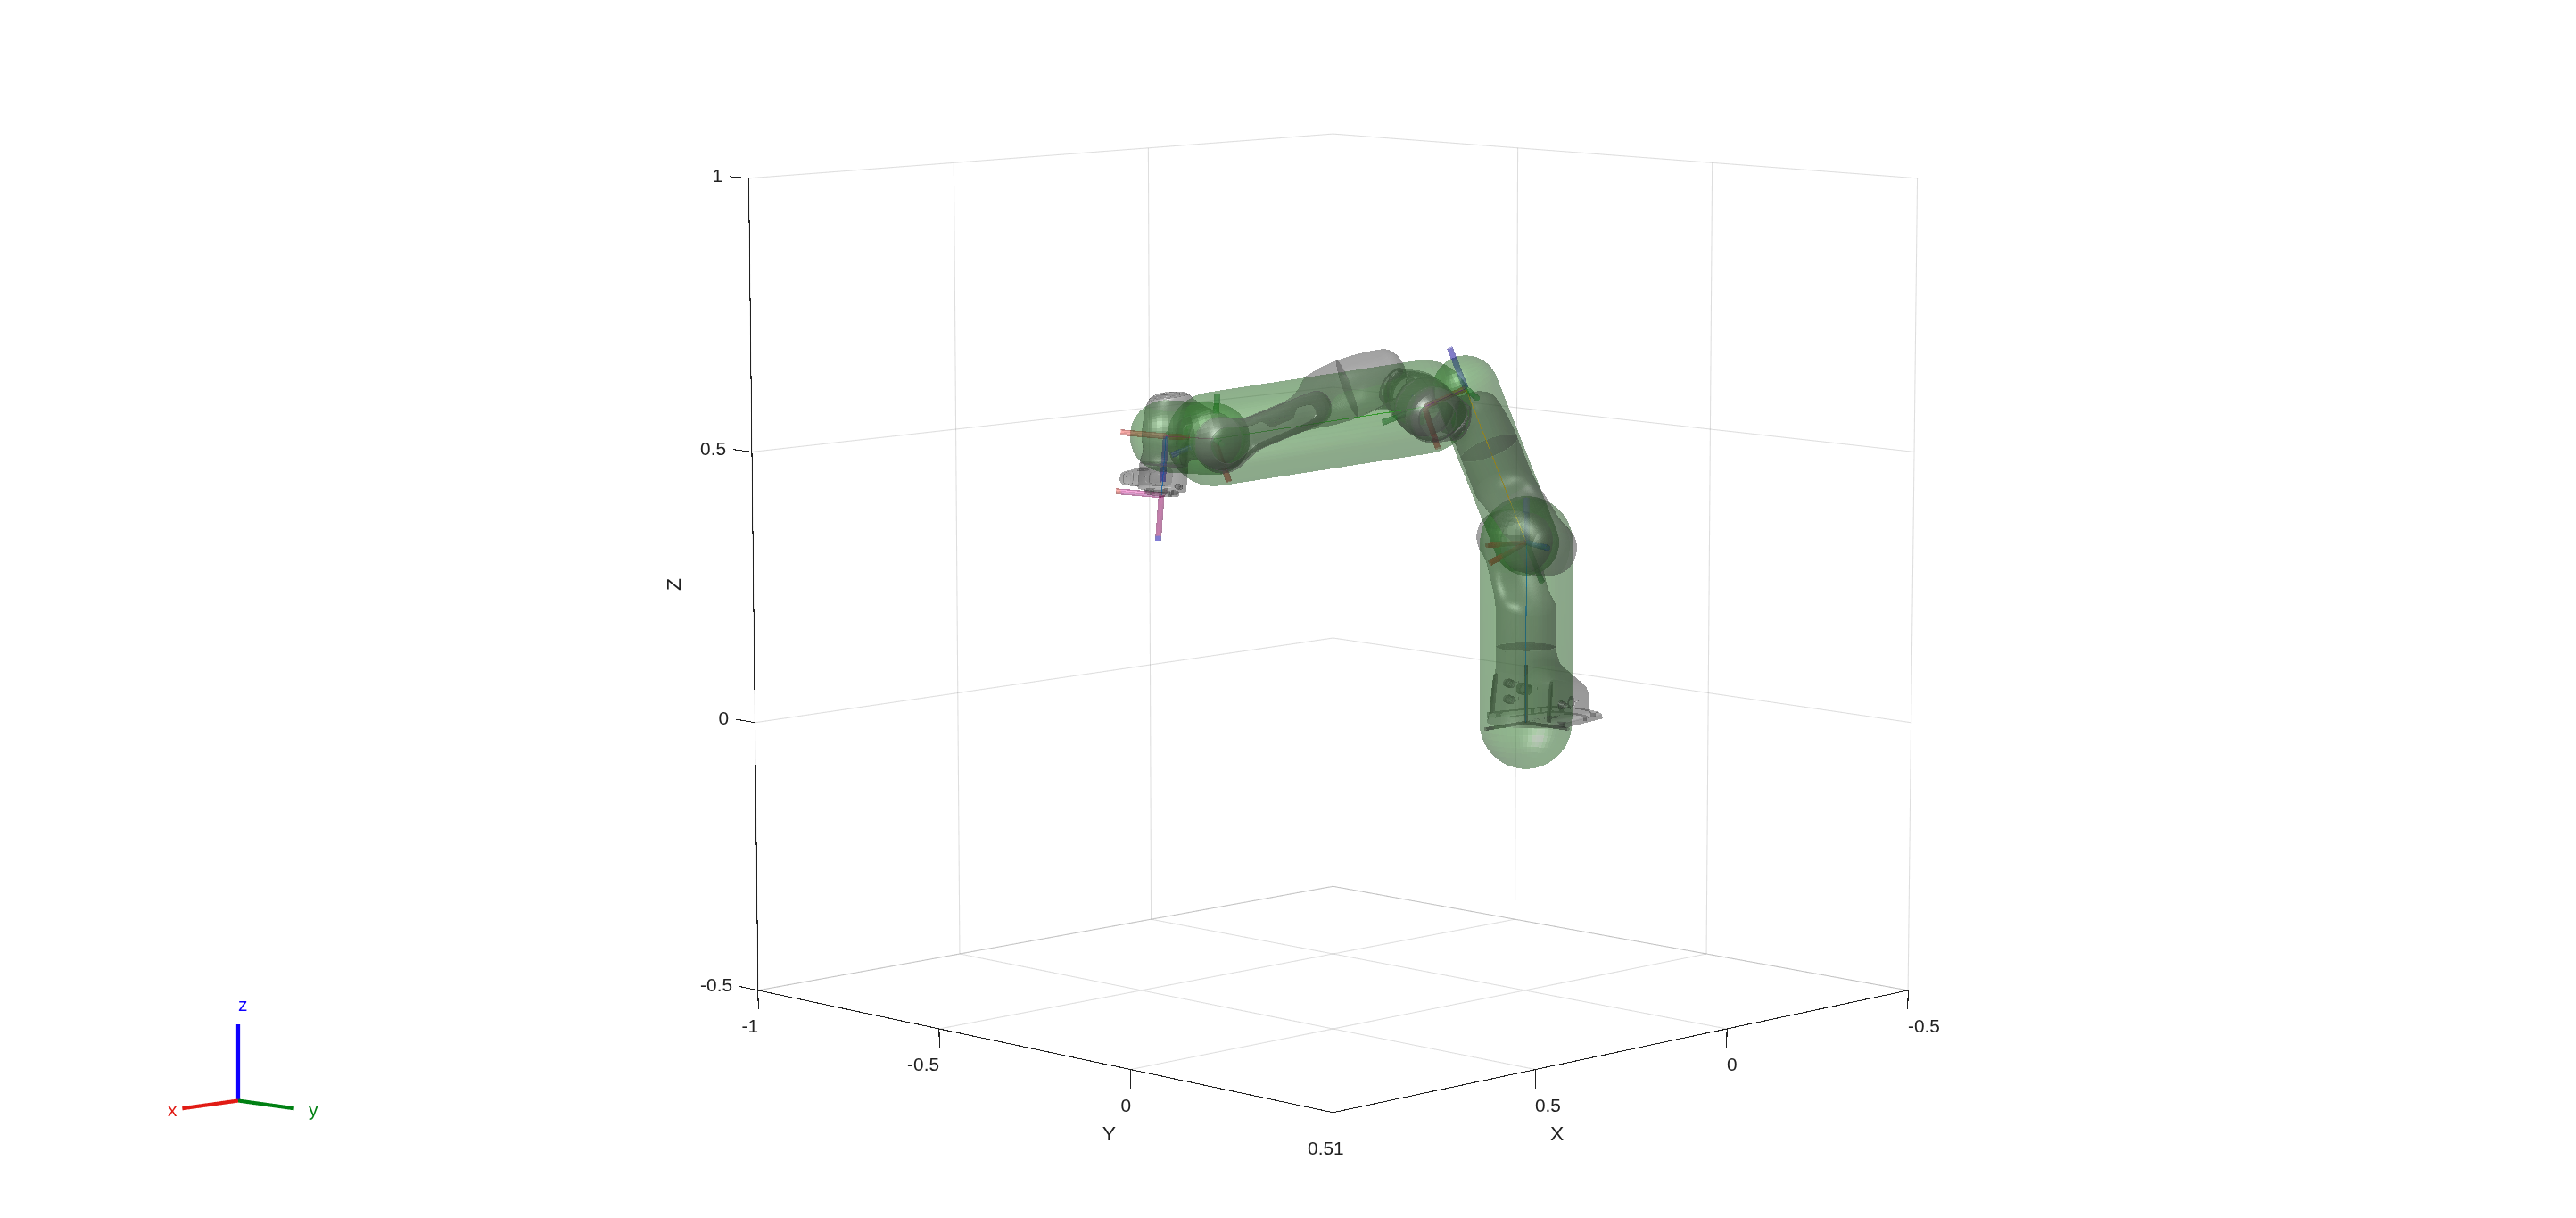
\includegraphics[width=\textwidth]{figure_tesi/robot_capsule.png}
        \caption{Modellazione geometrica tramite SSL}
        \label{fig:robot_capsule}
    \end{subfigure}
    \caption{Confronto tra la geometria dettagliata del robot (a) e la sua rappresentazione semplificata a capsule (b).} 
    \label{fig:robot_modellazione}
\end{figure}

In modo analogo, l'operatore umano viene modellato attraverso una scomposizione geometrica basata sullo scheletro tridimensionale rilevato dal sistema di visione. Tramite opportuni algoritmi di \textit{skeleton tracking} viene fornito un insieme ordinato di punti 3D corrispondenti alle principali articolazioni anatomiche (testa, spalle, gomiti, polsi, anche). Tali punti vengono utilizzati come estremi dei segmenti su cui vengono definite le SSL associate alle diverse parti del corpo dell'operatore.

\section{Distanza geometrica tra robot e operatore}

Come introdotto nella sezione precedente, sia il robot che l'operatore umano vengono approssimati tramite insiemi di primitive geometriche a capsula (SSL). Di conseguenza, la determinazione della distanza minima di sicurezza si riconduce al problema geometrico del calcolo della distanza minima tra i segmenti nello spazio tridimensionale $\mathbb{R}^3$, a cui viene successivamente sottratta la somma dei rispettivi raggi.

Si considerino due segmenti $S_1$ e $S_2$, individuati dalle rispettive coppie di estremi $(P_1, Q_1)$ e $(P_2, Q_2)$. Qualsiasi punto appartenente alle rette su cui giacciono tali segmenti può essere espresso in forma parametrica come:
\begin{align}
    \pmb{L_1(s)} &= \pmb{P_1} + s\pmb{D_1}, \quad \text{con } \pmb{D_1} = \pmb{Q_1} - \pmb{P_1} \\
    \pmb{L_2(t)} &= \pmb{P_2} + t\pmb{D_2}, \quad \text{con } \pmb{D_2} = \pmb{Q_2} - \pmb{P_2}
\end{align}
dove $s, t \in \mathbb{R}$ sono i parametri di linea. I punti appartengono ai segmenti fisici $S_1$ e $S_2$ se e solo se i rispettivi parametri soddisfano i vincoli $s \in [0,1]$ e $t \in [0, 1]$.

Definito il vettore di connessione tra le origini dei due segmenti $\pmb{R} = \pmb{P_1} - \pmb{P_2}$, il vettore che unisce due punti generici sulle due rette è espresso da:
\begin{equation}
    \pmb{v}(s,t) = L_1(s) - L_2(t) = \pmb{R} + s\pmb{D_1} - t\pmb{D_2}.
\end{equation}

Il problema di minima distanza equivale a minimizzare la norma al quadrato $||\pmb{v}(s,t)||^2$. Impostando le condizioni di ortogonalità del segmento di minima distanza rispetto alle direzioni dei due segmenti, ovvero $\pmb{v} \cdot \pmb{D_1} = 0$ e $\pmb{v} \cdot \pmb{D_2} = 0$, si ottiene un sistema di equazioni lineari il cui annullamento fornisce i valori ottimi dei parametri per le rette non parallele:
\begin{equation}
    s = \frac{(\pmb{D_1} \cdot \pmb{D_2})(\pmb{D_2} \cdot \pmb{R}) - (\pmb{D_2} \cdot \pmb{D_2})(\pmb{D_1} \cdot \pmb{R})}{(\pmb{D_1} \cdot \pmb{D_1})(\pmb{D_2} \cdot \pmb{D_2}) - (\pmb{D_1} \cdot \pmb{D_2})^2}
\end{equation}
\begin{equation}
    t = \frac{(\pmb{D_1} \cdot \pmb{D_1})(\pmb{D_2} \cdot \pmb{R}) - (\pmb{D_1} \cdot \pmb{D_2})(\pmb{D_1} \cdot \pmb{R})}{(\pmb{D_1} \cdot \pmb{D_1})(\pmb{D_2} \cdot \pmb{D_2}) - (\pmb{D_1} \cdot \pmb{D_2})^2}
\end{equation}

Qualora i valori di $s$ e $t$ così calcolati rientrino entrambi nell'intervallo $[0,1]$, i punti di minima distanza $C_1$ e $C_2$ si trivano all'interno dei segmenti e sono definiti da:
\begin{align}
    C_1 &= L_1(s) = \pmb{P_1} + s\pmb{D_1} \\
    C_2 &= L_2(t) = \pmb{P_2} + t\pmb{D_2}
\end{align}

Nel caso in cui uno o entrambi i parametri giacciano all'esterno dell'intervallo $[0,1]$, i punti di minima distanza si trovano sui bordi di almeno uno dei due segmenti. In tale eventualità, si satura il parametro fuori limite all'estremo più vicino, cioè $0$ o $1$, e si ricalcola analiticamente il valore dell'altro parametro mediante proiezione ortogonale sul relativo segmento, garantendo così il rispetto dei vincoli geometrici.

Come mostrato in Figura \ref{fig:distanze_segmenti}, trovati i due punti di minima distanza $C_1$ e $C_2$, la distanza euclidea tra i segmenti centrali risulta:
\begin{equation}
    d_{\text{seg}} = ||C_1 - C_2||
\end{equation}

In conclusione, la distanza effettiva $d_{\text{SSL}}$ tra le due primitive geometriche a capsula, caratterizzate dai rispettivi raggi $r_1$ e $r_2$, è ricavata sottraendo i due raggi dei volumi di ingombro:
\begin{equation}
    d_{\text{SSL}} = \max(0, \; d_{text{seg}} - r_1 -r_2)
\end{equation}

\begin{figure}
    \centering
    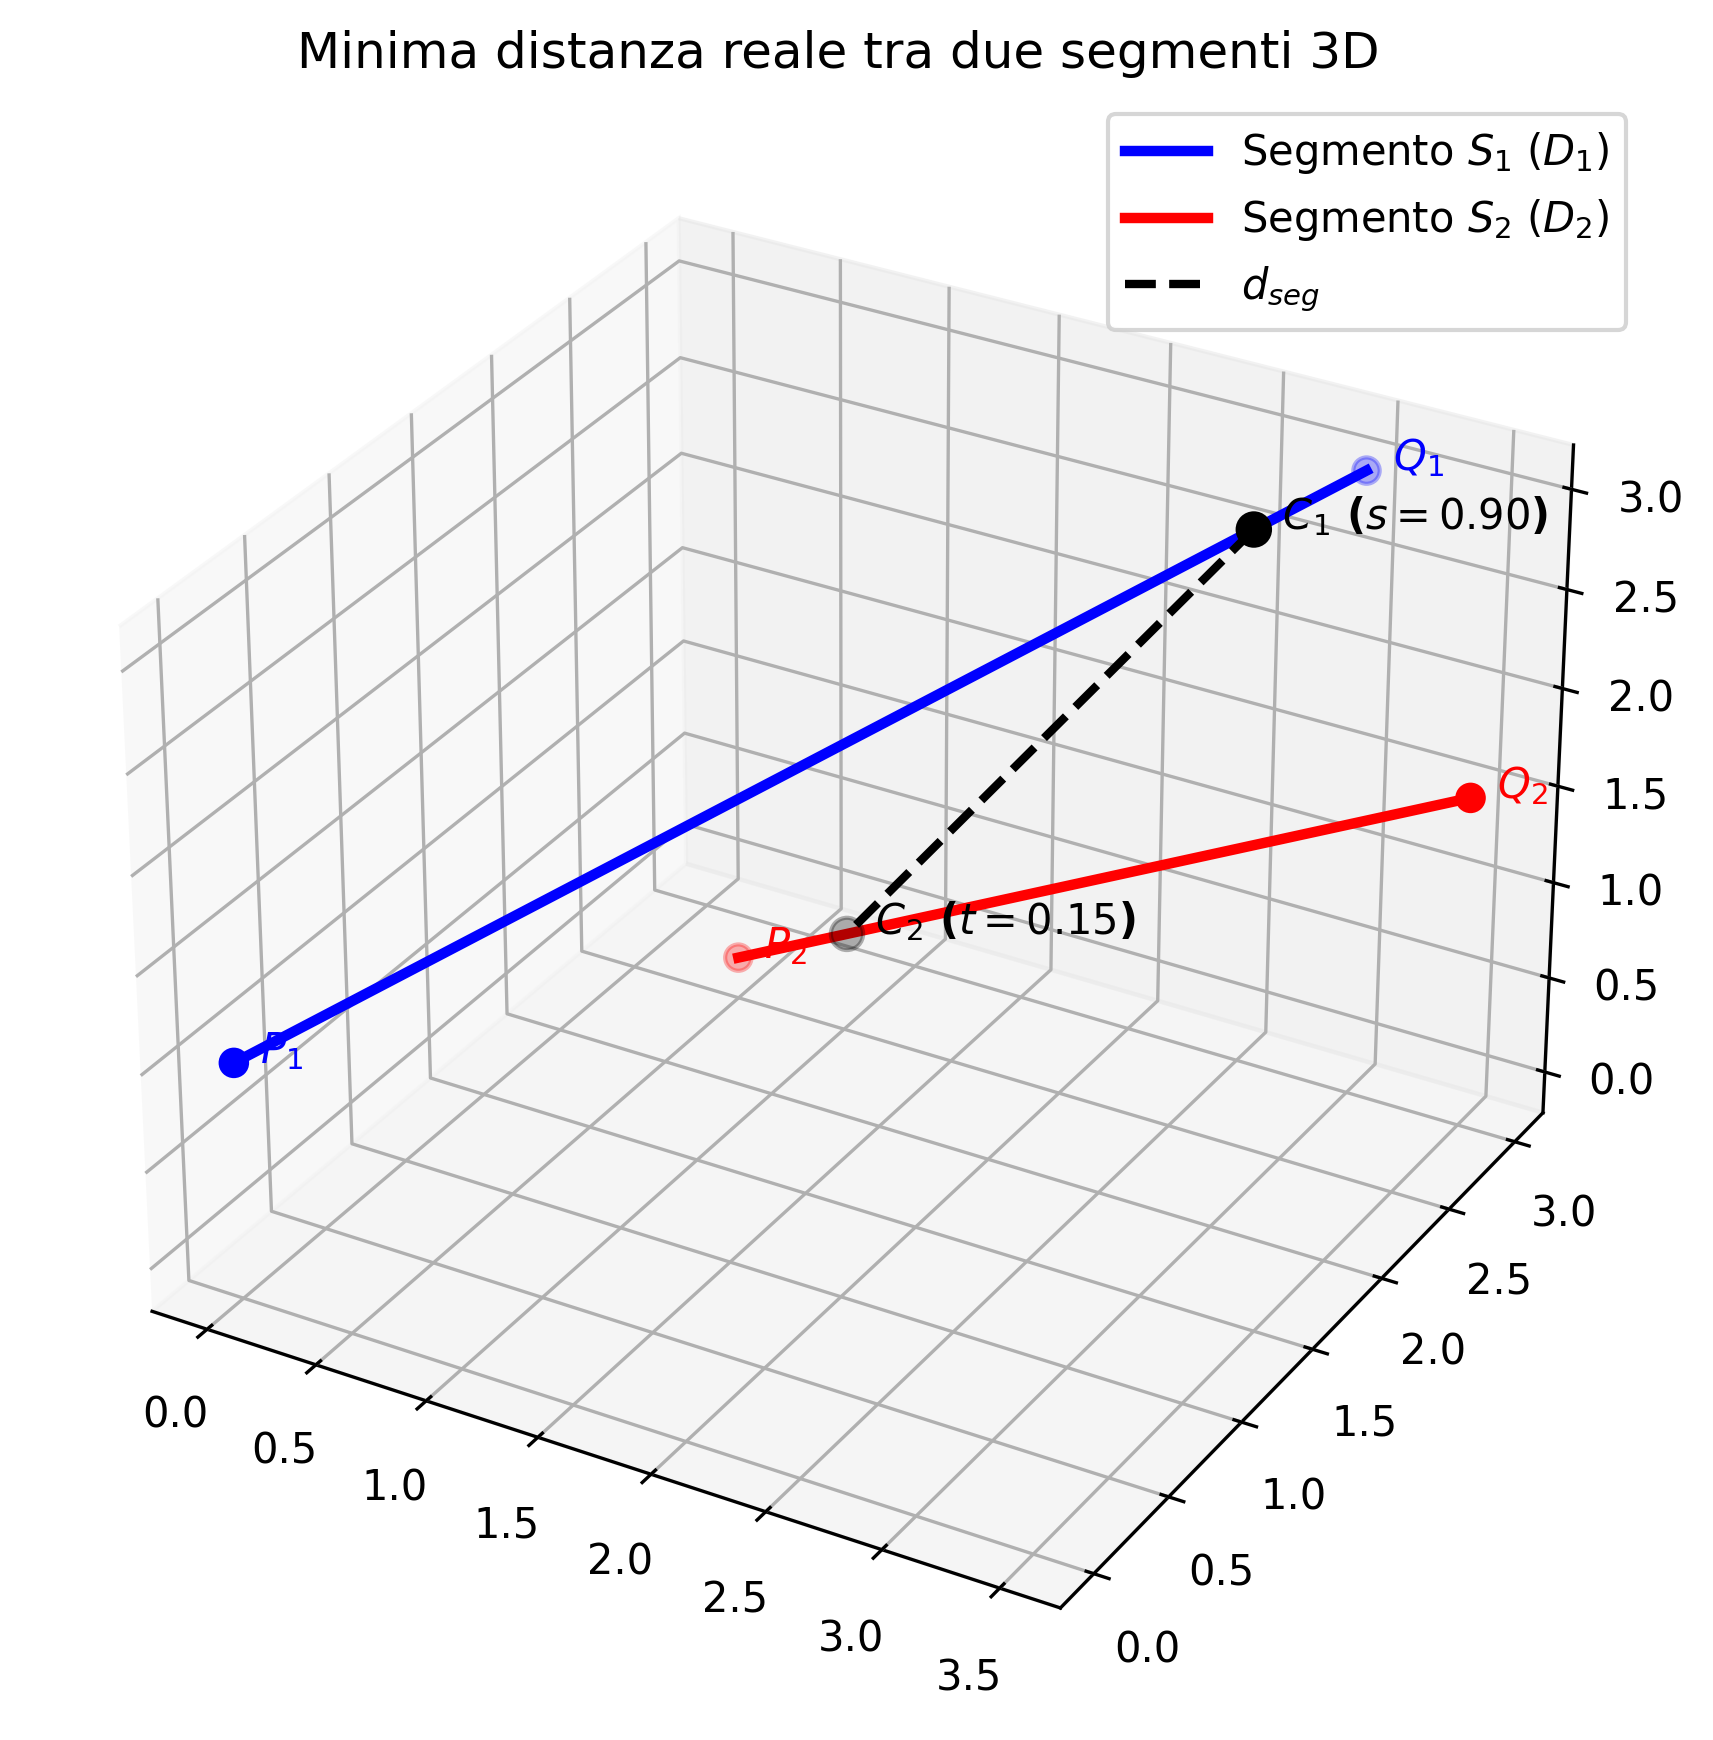
\includegraphics[width=0.5\linewidth]{figure_tesi/distanza_segmenti_corretta.png}
    \caption{Rappresentazione geometrica della distanza minima $d_{seg}$ tra due segmenti $S_1$ e $S_2$.}
    \label{fig:distanze_segmenti}
\end{figure}

\section{Primo approccio: dimensionamento dinamico delle zone di sicurezza}
\label{sec:primo_approccio}

Questo approccio alla collaborazione uomo-robot in sicurezza si basa sul principio di \textit{Speed and Separation Monitoring} (SSM). Per superare la rigidità dei metodi convenzionali con zone di sicurezza fisse o sovradimensionate, il sistema ottimizza online il tempo di arresto $T_{\text{stop}}$. 

\subsection{Principio dello Speed and Separation Monitoring (SSM)}
Secondo le direttive della specifica tecinca ISO/TS 15066 \cite{ISO15066}, la modalità di collaborazione SSM impone che la velocità operativa del manipolatore sia continuamente regolata in funzione della distanza relativa dall'operatore umano. L'obiettivo principale è garantire che la distanza di separazione corrente $S(t)$ tra qualsiasi punto del robot e l'operatore non sia mai inferiore a una distanza di sicurezza minima $S_{\text{min}}(t)$, definita come:
\begin{equation}
    S_{\text{min}}(t) = S_h(t) + S_r(t) + S_s(t) + C + Z_d + Z_r
    \label{eq:iso_ssm_distance}
\end{equation}
dove:
\begin{itemize}
    \item $S_h(t)$ rappresenta lo spostamento potenziale dell'operatore verso il robot durante la fase di reazione ed esecuzione dell'arresto;
    \item $S_r(t)$ è lo spazio percorso dal robot durante il tempo di reazione del sistema di controllo $t_r$;
    \item $S_s(t)$ rappresenta lo spazio effettivo di frenata del manipolatore;
    \item $C$, $Z_d$ e $Z_r$ sono termini cautelativi legati rispettivamente alle capacità di intrusione dell'operatore, alle incertezze dei sensori di tracciamento e alla tolleranza di posizionamento del robot.
\end{itemize}

Nei sistemi tradizionali, le componenti $S_s(t)$ e $S_r(t)$ vengono calcolate assumendo le peggiori condizioni cinematiche e dinamiche possibili (es. massima velocità e carico nominale), conducendo a distanze $S_{\text{min}}$ costanti, conservative e fortemente penalizzanti per la produttività. Per superare tale rigidità, il metodo qui descritto propone un'ottimizzazione in tempo reale del tempo di arresto $T_{\text{stop}}$, consentendo la generazione di capsule protettive dinamiche e adeguate all'effettivo stato cinematico del robot. La stima accurata di $T_{\text{stop}}$ consente di determinare l'effettivo spazio di frenata e di ridimensionare dinamicamente le capsule di sicurezza protettive, modellate come \textit{Sphere Swept Lines} (SSL), attorno ai bracci del manipolatore.

\subsection{Pianificazione online della traiettoria di arresto}
\label{subsec:traiettoria_stop}
Al momento della rilevazione di un potenziale rischio di collisione al generico istante temporale $t_0$, il controllore non applica un'interruzione discontinua della traiettoria nominale. Viene invece generata online una traiettoria di arresto continua e differenziabile del dominio dei giunti per evitare sollecitazioni impulsive sui riduttori. 

Si definisce $t_r$ il tempo di reazione dell'architettura di controllo. la manovra di frenata s sviluppa nell'intervallo temporale $t \in [t_i, t_f]$ dove $t_i = t_0 + t_r$ rappresenta l'istante di innesco reale della frenata e $t_f = t_0+t_r+T_{\text{stop}}$ specifica l'istante di arresto completo \cite{Scalera2024}.

Per imporre la continuità di posizione, velocità e accelerazione, la traiettoria di arresto $q_j(t)$, per $j = 1, \dots, 7$, viene descritta tramite un polinomio del $5^\circ$ grado \cite{Scalera2024}, per ciascuno dei $7$ giunti del manipolatore, :
\begin{equation}
    q_j(t) = a_0+a_1t+a_2t^2+a_3t^3+a_4t^4+a_5t^5
\end{equation}

I coefficienti $a_k$, per $k = 0, \dots, 5$, del polinomio vengono determinati analiticamente in tempo reale imponendo le condizioni al contorno tra lo stato cinematico iniziale di frenata al tempo $t_i$ e lo stato di arresto completo al tempo $t_f$:
\begin{equation}
    \begin{cases}
        q_j(t_i)=q_{i,j}, & q_j(t_f)=q_{i,j} \\
        \dot{q}_j(t_i)= \dot{q}_{i,j}, & \dot{q}_j(t_f) = 0 \\
        \ddot{q}_j(t_i) = \ddot{q}_{i,j}, & \ddot{q}_j(t_f) = 0
    \end{cases}
\end{equation}

\begin{figure}[htbp]
    \centering
    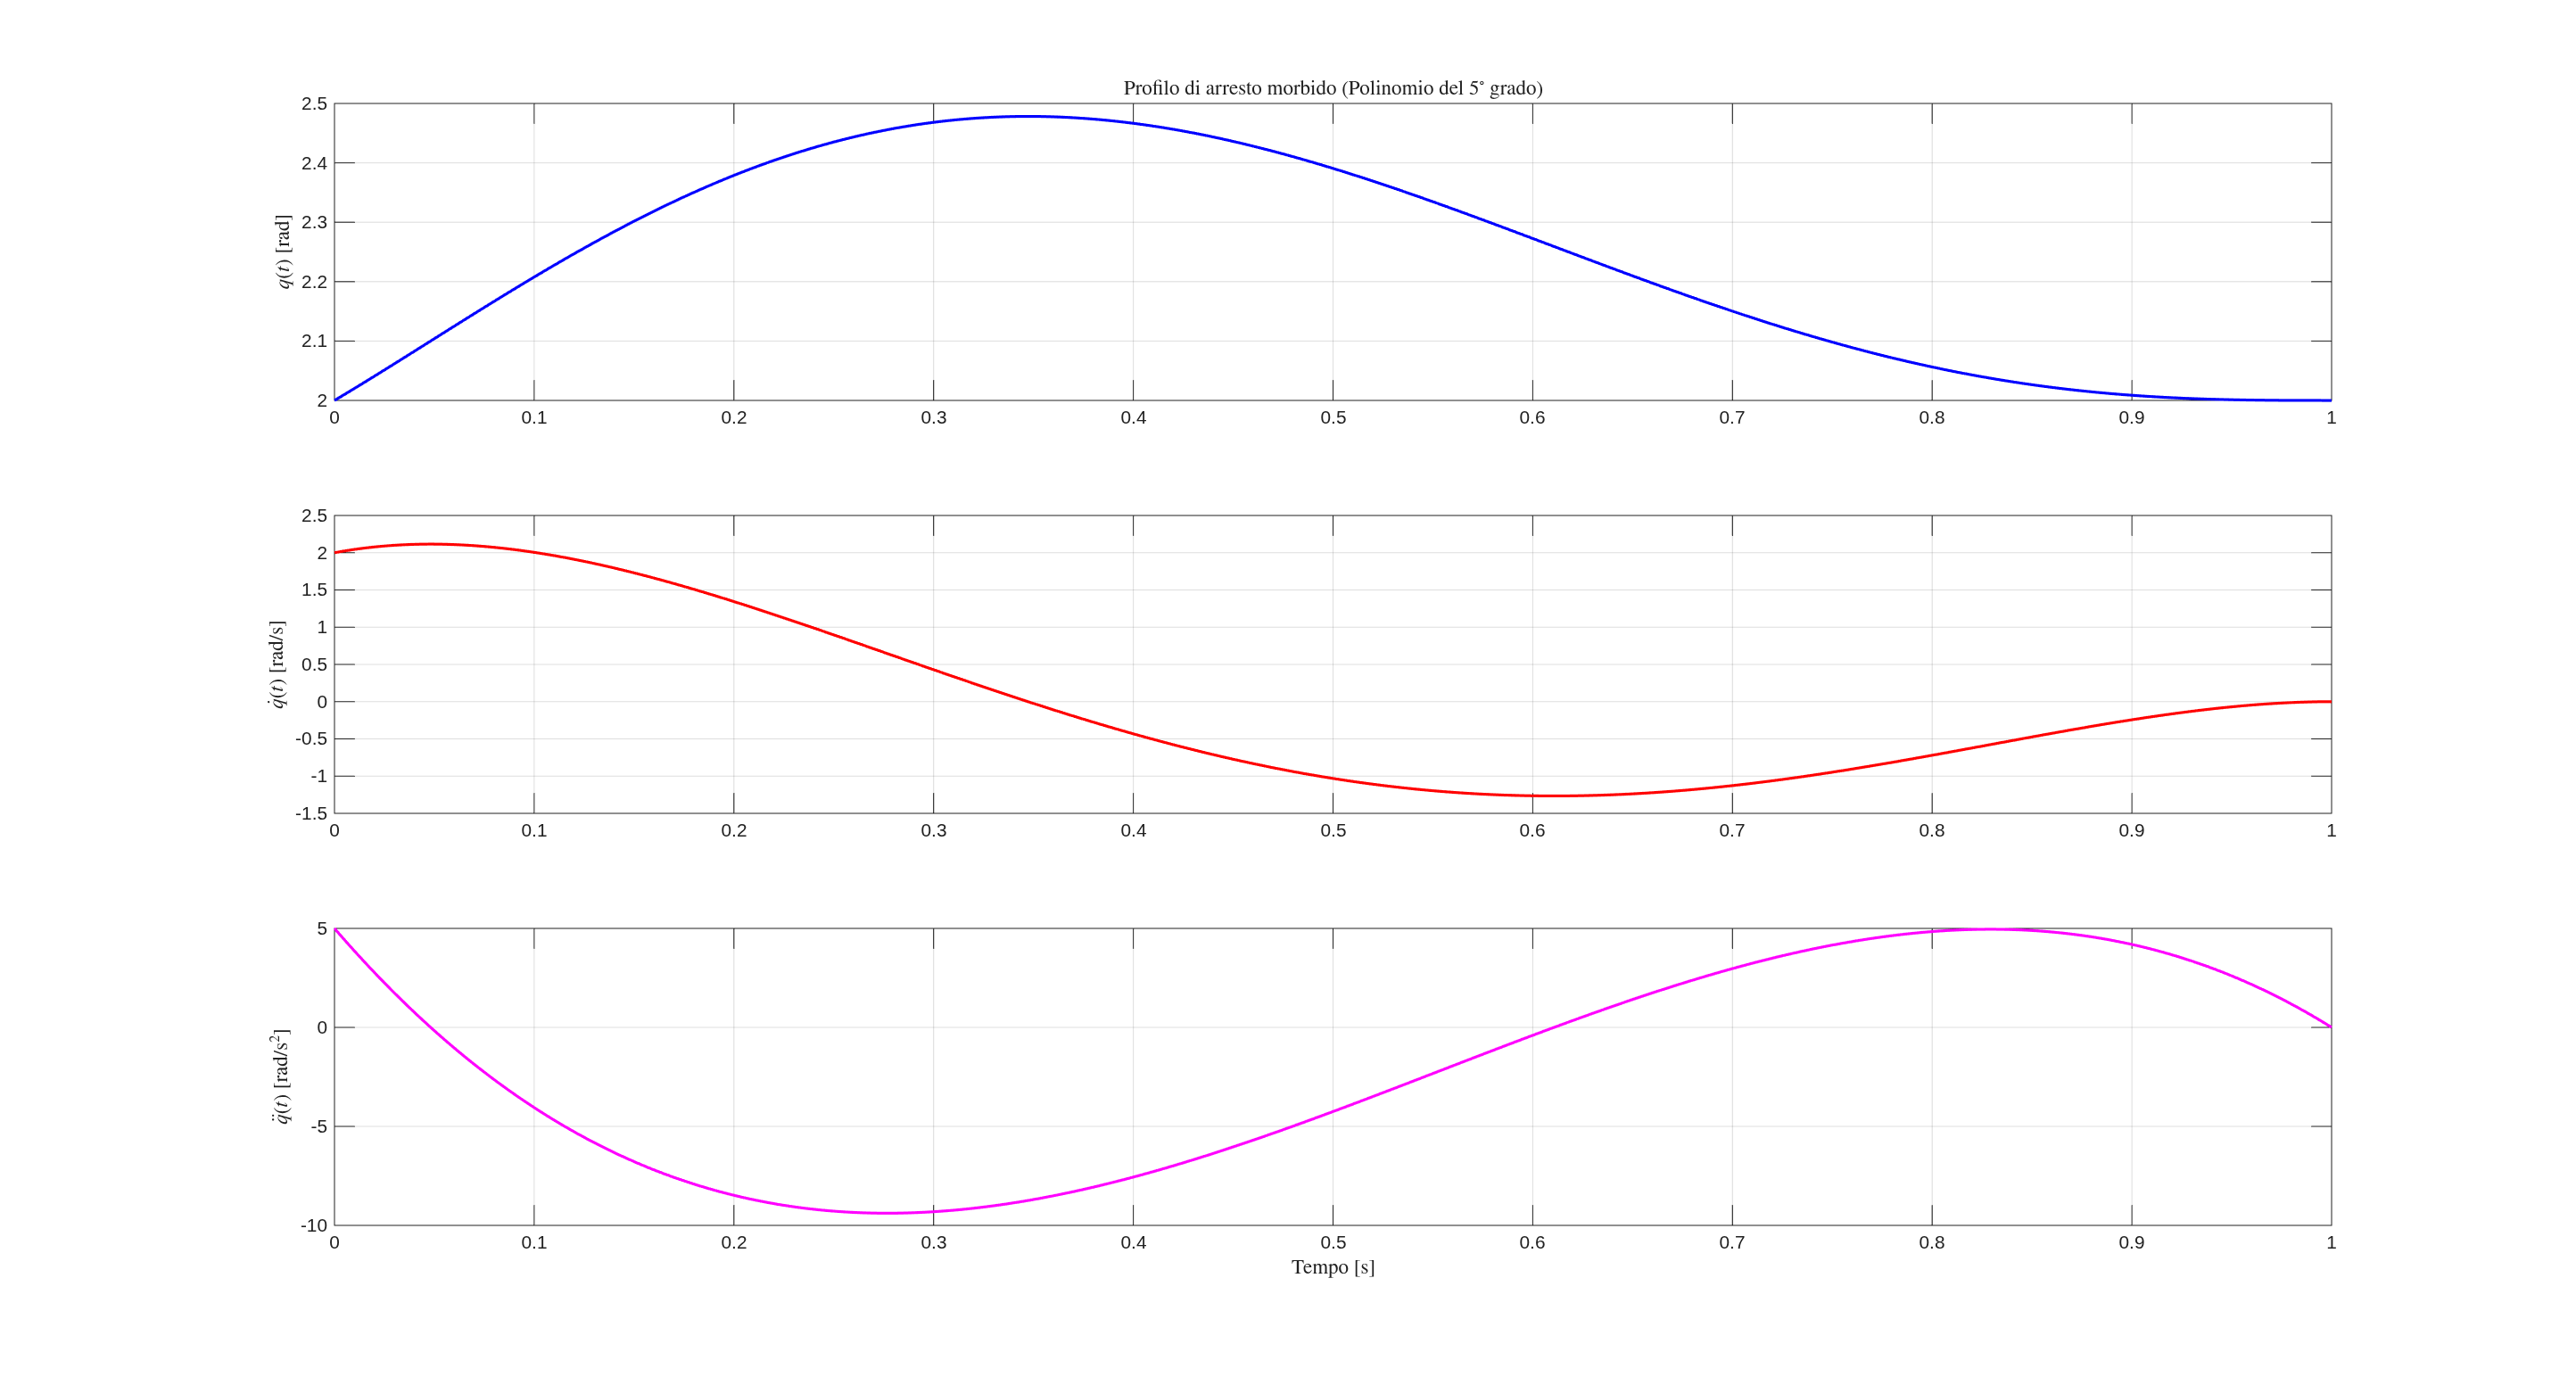
\includegraphics[width=1\linewidth]{figure_tesi/arresto_morbido.png}
    \caption{Profili temporali di posizione $q(t)$, velocità $\dot{q}(t)$ e accelerazione $\ddot{q}(t)$ durante la manovra di arresto morbido con polinomio quintico.}
    \label{fig:arresto_morbido}
\end{figure}

Si noti che in questa formulazione si impone che la posizione obiettivo di arresto al tempo $t_f$ corrisponda alla posizione $q_{i,j}$ registrata all'istante di innesco della frenata, come si può notare dalla Figura~\ref{fig:arresto_morbido}. Sarà compito della pianificazione polinomiale quintica garantire la continuità e la sicurezza dell'arresto lungo l'intervallo $T_{\text{stop}}$, gestendo la transizione a partire dalla velocità iniziale non nulla $\dot{q}_{i,j} \neq 0$.



\subsection{Formulazione dell'ottimizzazione e vincoli dinamici}
\label{subsec:optimization_problem}
La determinazione del tempo di arresto minimo $T_{\text{stop}}$ viene formulata come un problema di ottimizzazione vincolata ad ogni passo di controllo \cite{Scalera2024, Scalera2022}:
\begin{equation}
    \min_{T_{\text{stop}}} \quad w_0 T_{\text{stop}} + w_1 \left|T_{\text{stop}}-T_{\text{stop,prev}} \right|
    \label{eq:funzione_costo}
\end{equation}
dove $w_0, w_1 > 0$ sono pesi di ponderazione e $T_{\text{stop,prev}}$ rappresenta la soluzione computata al ciclo precedente. La presenza del termine penalizzante $|T_{\text{stop}} - T_{\text{stop,prev}}|$ introduce un'azione di regolarizzazione, garantendo continuità temporale nelle dimensioni delle capsule ed evitando variazioni brusche dell'area di ingombro tra iterazioni successive.

L'ottimizzazione dell'equazione \ref{eq:funzione_costo} è soggetta al rispetto stringente dei limiti cinematici e dinamici del manipolatore per tutta la durata della frenata, $\forall t \in [t_i, t_f]$:
\begin{align}
    |\dot{q}_j(t)| &\le \dot{q}_{j,\max} \quad &\forall j=1, \dots, 7 \label{eq:vel_lim}\\
    |\ddot{q}_j(t)| &\le \ddot{q}_{j,\max} \quad &\forall j=1, \dots, 7 \label{eq:acc_lim}\\
    |\dddot{q}_j(t)| &\le \dddot{q}_{j,\max} \quad &\forall j = 1, \dots, 7 \label{eq:jerk_lim}\\
    |\tau_j(t)| &\le \tau_{j,\max} \quad &\forall j = 1, \dots, 7 \label{eq:torque_lim}\\
    |\dot{\tau}_j(t)| &\le \dot{\tau}_{j,\max} \quad &\forall j = 1, \dots, 7 \label{eq:dtorque_lim}
\end{align}

Il vettore delle coppie ai giunti $\tau(t) \in \mathbb{R}^n$ è legato allo stato cinematico attraverso il modello dinamico inverso dell'equazione di Lagrange:
\begin{equation}
    \tau(t) = M(q)\ddot{q} + C(q, \dot{q})\dot{q} + g(q)
\end{equation}
In cui $M(q) \in \mathbb{R}^{7 \times 7}$ rappresenta la matrice d'inerzia, $C(q, \dot{q} \in \mathbb{R}^{7 \times 7}$ include i termini centripeti e di Coriolis e $g(q) \in \mathbb{R}^7$ è il vettore delle forze di gravità.

Attraverso la soluzione dell'equazione \eqref{eq:funzione_costo}, il sistema calcola il tempo di frenata minimo ammissibile. Ciò consente di modellare capsule di sicurezza protettive con l'ingombro spaziale strettamente necessario, massimizzando lo spazio di 
lavoro condiviso ed evitando arresti non necessari durante l'esecuzione del task.

\section{Secondo approccio: capsule \textit{soft}}

Per minimizzare le interruzioni operative e garantire una continuità di servizio nello spazio di lavoro collaborativo, il secondo approccio introduce l'impiego di capsule \textit{soft}. Rispetto ai volumi di ingombro impiegati per la gestione degli arresti di sicurezza, queste capsule presentano dimensioni in generale maggiori e definiscono una fascia di interazione dinamica tra il robot e l'operatore umano. In questo scenario, un'eventuale intersezione tra le capsule del manipolatore e le \textit{Sphere Swept Lines} (SSL) associate all'operatore non determina un arresto immediato del sistema, ma innesca una strategia di evasione attiva basata sul ricalcolo in tempo reale della traiettoria del task\cite{Qyrani2026}.

\subsection{Confronto tra capsule \textit{hard} e \textit{soft}}

Per armonizzare i requisiti di produttività e sicurezza, questa architettura prevede l'adozione simultanea di due set concentrici di capsule:

\begin{itemize}
    \item \textbf{Capsule \textit{hard}:} presentano dimensioni prossime al volume d'ingombro fisico del manipolatore e svolgono una funzione puramente protettiva. Come descritto nella Sezione~\ref{sec:primo_approccio}, una loro eventuale intersezione con le SSL dell'operatore indica una violazione dei margini minimi di sicurezza e comporta l'attivazione immediata dell'arresto con traiettoria di frenata morbida a profilo quintico.
    \item \textbf{Capsule \textit{soft}:} possiedono un raggio maggiorato e sono vincolate alla struttura dei bracci robotici. Esse definiscono una zona di pre-allarme dinamica: la misura del grado di penetrazione o sovrapposizione con le SSL dell'operatore non arresta il robot, ma viene impiegata per sintesi e calcolo della forza repulsiva virtuale responsabile della deviazione di traiettoria.
\end{itemize}

L'azione combinata dei due set garantisce che il robot cerchi prima di evitare attivamente l'operatore tramite le capsule \textit{soft} e, solo nel caso in cui l'evasione non sia sufficiente a prevenire la violazione delle capsule \textit{hard}, intervenga la procedura di arresto sicuro.

\subsection{Controllo di ammettenza per l'evasione dinamica}

Il ricalcolo della traiettoria in tempo reale si fonda sull'implementazione di uno schema di controllo di ammettenza nello spazio cartesiano. Nell'ambito del controllo dell'interazione, la letteratura distingue tra approcci d'impedenza e d'ammettenza in base alle relazioni di causalità adottate:
\begin{itemize}
    \item \textbf{Controllo d'impedenza (Causalità Moto $\rightarrow$ Forza):} accetta un errore/deviazione di posizione come ingresso e calcola la forza o coppia di reazione da applicare al robot.
    \item \textbf{Controllo d'ammettenza (Causalità Forza $\rightarrow$ Moto):} misura o sintetizza una forza esterna come ingresso e la converte in un riferimento di moto (posizione, velocità e accelerazione).
\end{itemize}

Poiché i controllori industriali standard e le API di basso livello del robot sono tipicamente ottimizzati con anelli interni di posizione e velocità ad elevata rigidezza, il controllo d'ammettenza risulta l'approccio ideale. Esso agisce come un filtro dinamico esterno che genera un nuovo riferimento cinematico inviabile direttamente ai servocomandi di giunto del manipolatore.

\subsubsection{Sintesi della forza repulsiva e dinamica dell'ammettenza}

Nel nostro scenario di evasione non si ha un contatto fisico reale con l'operatore; la vicinanza dell'uomo all'interno della capsula \textit{soft} viene tradotta in una forza repulsiva virtuale $\boldsymbol{F}_{\text{rep}} \in \mathbb{R}^6$. Tale forza ha modulo proporzionale alla profondità di penetrazione all'interno della fascia \textit{soft} ed è diretta lungo la retta di minima distanza tra i segmenti geometrici.

La forza virtuale $\boldsymbol{F}_{\text{rep}}$ viene fornita in ingresso al modello dell'ammettenza cartesiana, che modella l'interfaccia di contatto come un sistema meccanico equivalente di tipo massa-molla-smorzatore:
\begin{equation}
\boldsymbol{M}_d \big(\ddot{\boldsymbol{x}}_r - \ddot{\boldsymbol{x}}_d\big) + \boldsymbol{D}_d \big(\dot{\boldsymbol{x}}_r - \dot{\boldsymbol{x}}_d\big) + \boldsymbol{K}_d \big(\boldsymbol{x}_r - \boldsymbol{x}_d\big) = \boldsymbol{F}_{\text{rep}}
\label{eq:admittance_dynamics}
\end{equation}

dove:
\begin{itemize}
    \item $\boldsymbol{x}_d, \dot{\boldsymbol{x}}_d, \ddot{\boldsymbol{x}}_d \in \mathbb{R}^6$ indicano le grandezze cartesiane desiderate (posizione, velocità, accelerazione) pianificate dal task nominale. Lo spazio $\mathbb{R}^6$ viene adottato per descrivere completamente i 6 gradi di libertà del manipolatore nello spazio operativo, includendo sia le 3 componenti traslazionali sia le 3 componenti rotazionali dell'organo terminale;
    \item $\boldsymbol{x}_r, \dot{\boldsymbol{x}}_r, \ddot{\boldsymbol{x}}_r \in \mathbb{R}^6$ rappresentano lo stato di riferimento modificato che viene calcolato online;
    \item $\boldsymbol{M}_d, \boldsymbol{D}_d, \boldsymbol{K}_d \in \mathbb{R}^{6 \times 6}$ costituiscono le matrici simmetriche e definite positive di massa, smorzamento e rigidezza virtuali desiderate.
\end{itemize}

\subsubsection{Calcolo online della posizione modificata}

L'equazione~(\ref{eq:admittance_dynamics}) descrive un sistema differenziale del secondo ordine. Esplicitando il termine di accelerazione modificata $\ddot{\boldsymbol{x}}_r$, si ottiene:
\begin{equation}
\ddot{\boldsymbol{x}}_r = \ddot{\boldsymbol{x}}_d + M_d^{-1} \Big( \boldsymbol{F}_{\text{rep}} - D_d \big(\dot{\boldsymbol{x}}_r - \dot{\boldsymbol{x}}_d\big) - K_d \big(\boldsymbol{x}_r - \boldsymbol{x}_d\big) \Big)
\end{equation}

Attraverso schemi di integrazione numerica in tempo reale (es. Eulero o Runge-Kutta al ciclo di controllo a 1 kHz), questa accelerazione viene integrata passo-passo per ricavare la velocità $\dot{\boldsymbol{x}}_r(t)$ e infine la nuova posizione cartesiana di riferimento $\boldsymbol{x}_r(t)$. 

Il comportamento del robot durante l'evasione è governato dai parametri della matrice virtuale:
\begin{itemize}
    \item Azione della massa ($\boldsymbol{M}_d$): filtra i picchi improvvisi della forza repulsiva, garantendo accelerazioni fluide ed evitando scatti bruschi.
    \item Azione dello smorzamento ($\boldsymbol{D}_d$): dissipa l'energia del sistema virtuale e previene l'insorgere di oscillazioni indesiderate durante l'allontanamento dall'operatore.
    \item Azione della rigidezza ($\boldsymbol{K}_d$): agisce come un richiamo elastico verso la traiettoria nominale $\boldsymbol{x}_d(t)$. Nel momento in cui l'operatore esce dalla capsula \textit{soft}, la forza repulsiva $\boldsymbol{F}_{\text{rep}}$ si annulla e il termine $K_d$ riporta gradualmente e in modo fluido il robot sul percorso pianificato originario.
\end{itemize}

Infine, la posizione cartesiana modificata $\boldsymbol{x}_r(t)$ viene convertita nelle corrispondenti variabili di giunto $\boldsymbol{q}_r(t)$ tramite cinematica inversa differenziale (sfruttando lo Jacobiano analitico o geometrico del robot) e inviata all'anello di controllo di posizione interno.



\chapter{Implementazione}

\section{Braccio robotico}
Il manipolatore utilizzato in questa attività di tesi è il \textit{Franka Emika Panda} mostrato in Figura~\ref{fig:robot_reale}, un robot collaborativo a $7$ gradi di libertà costruito appositamente per l'interazione sicura con l'operatore umano.

\begin{figure} [htbp]
    \centering
    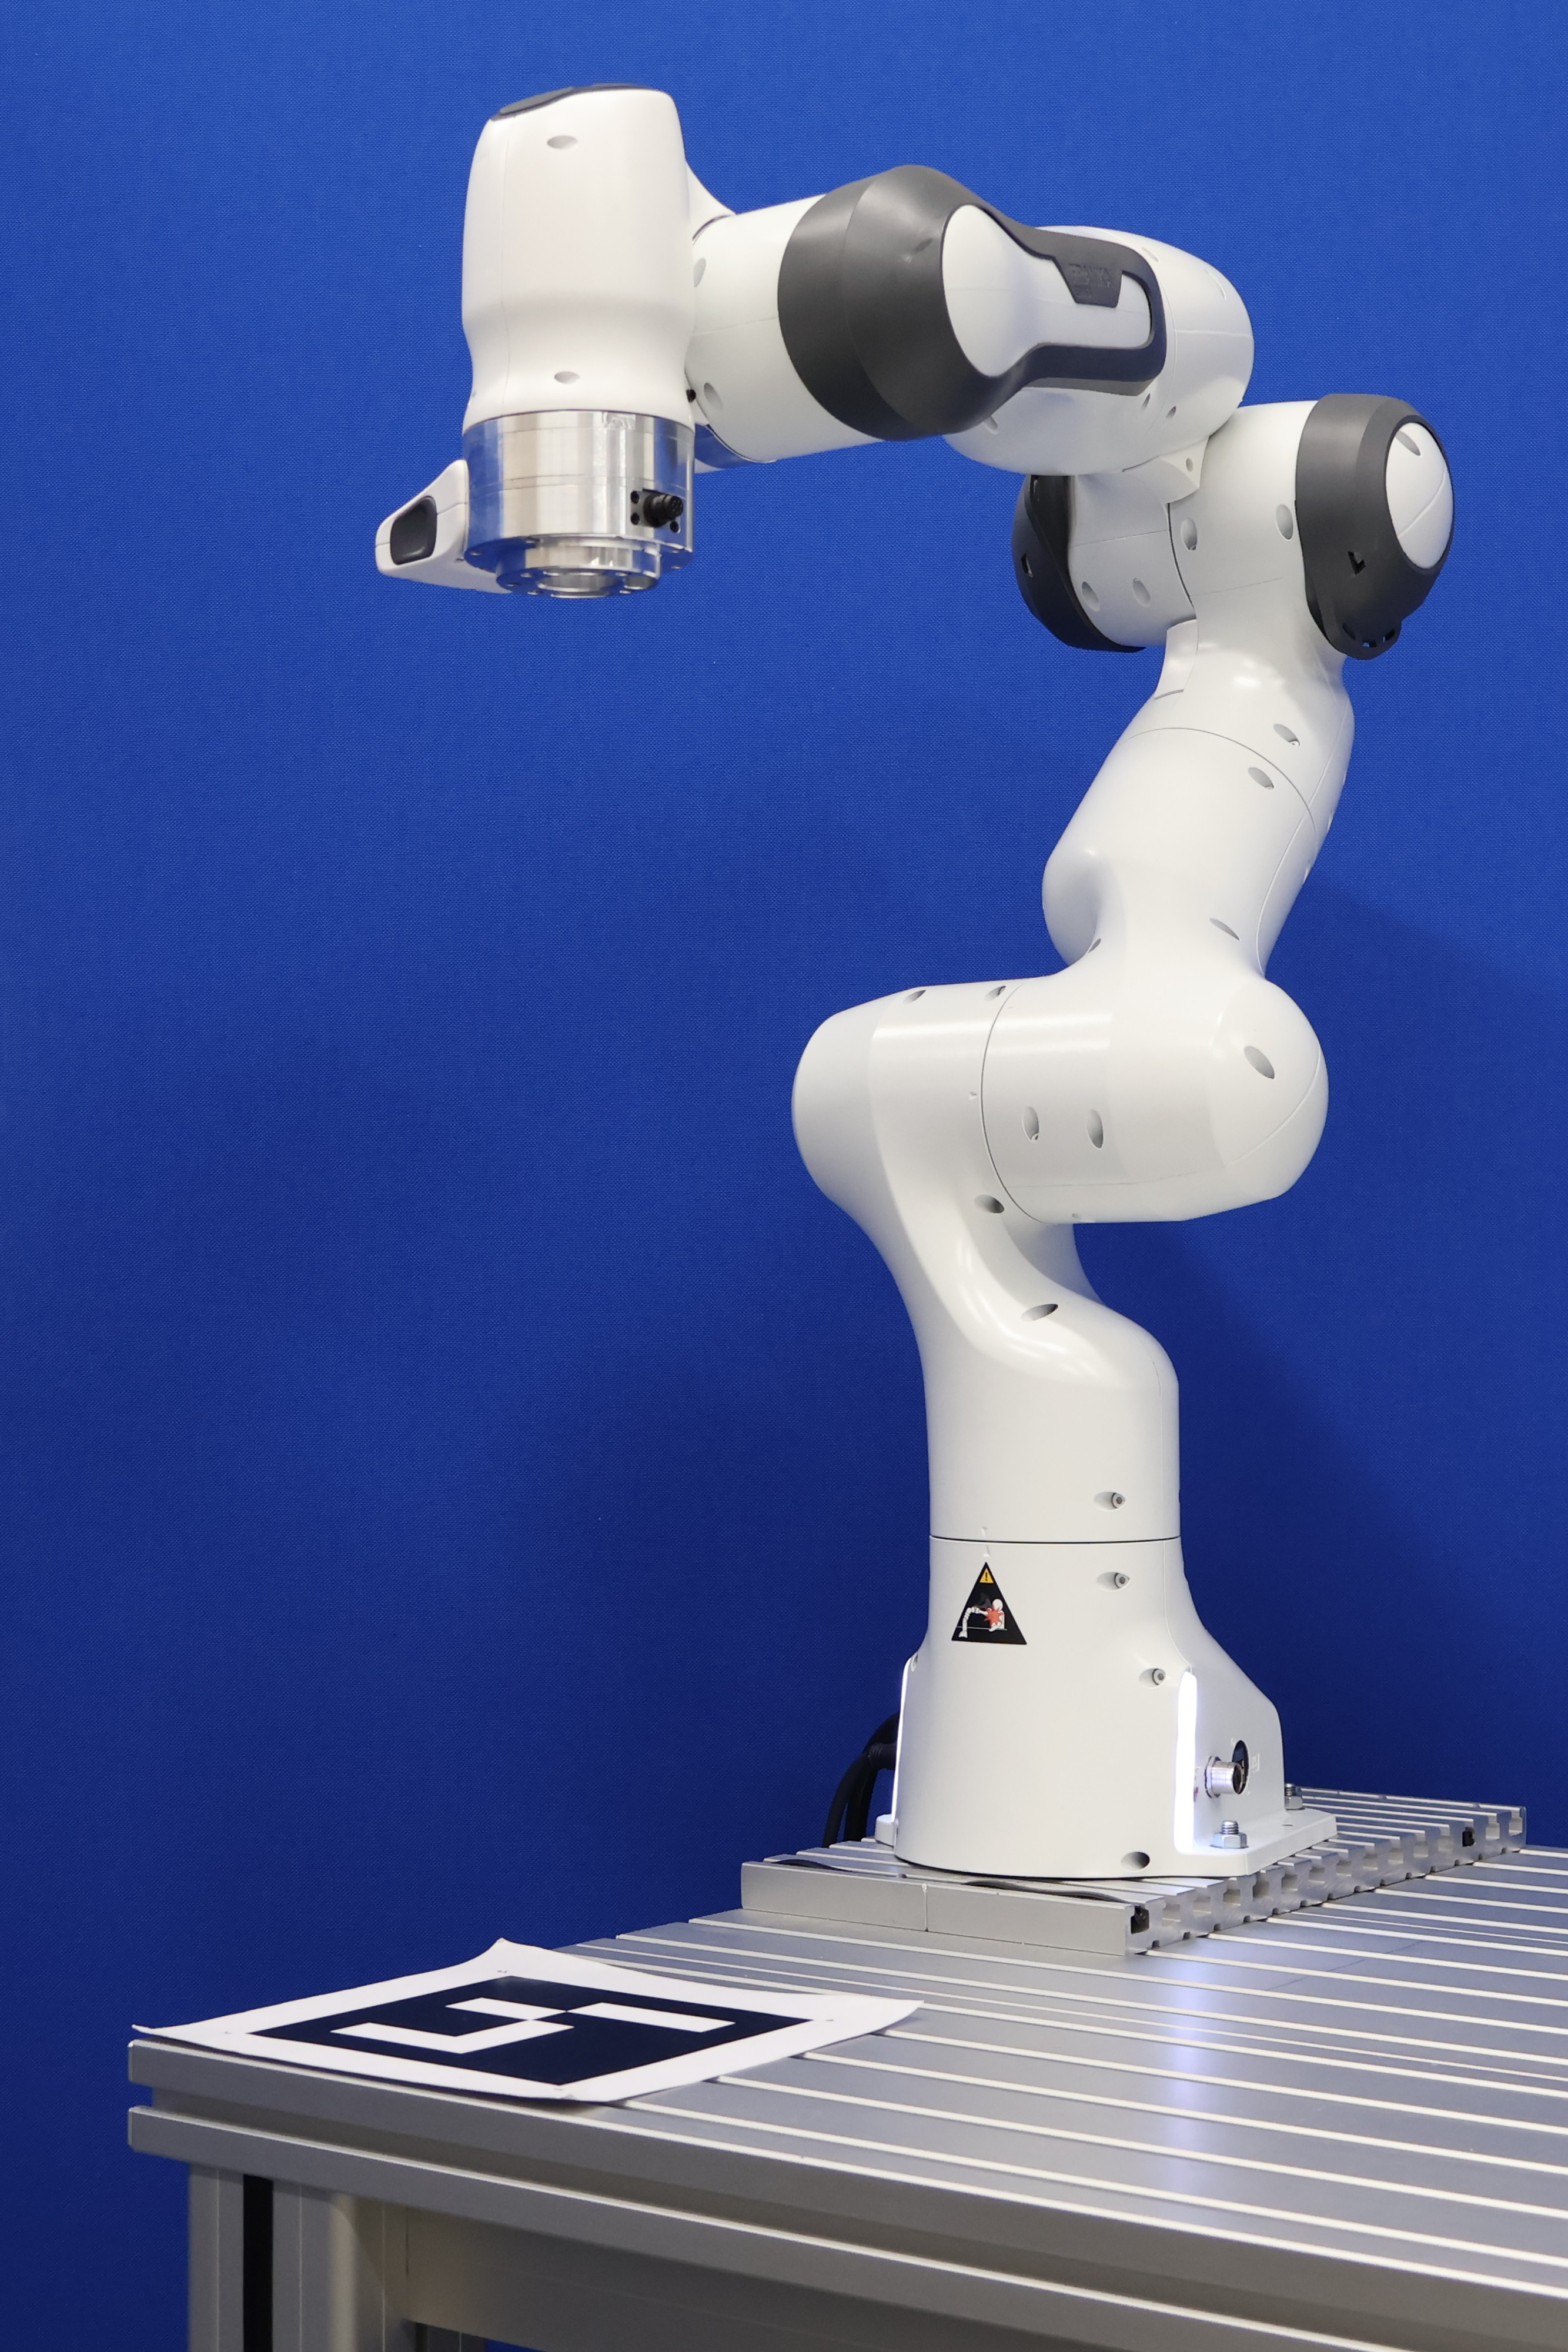
\includegraphics[width=0.4\linewidth]{figure_tesi/robot_reale.png}
    \caption{Robot collaborativo \textit{Franka Emika Panda}}
    \label{fig:robot_reale}
\end{figure}

Il robot ha una lunghezza massima di $850\text{ mm}$ e un carico utile \textit{payload} nominale di $3 \text{ kg}$. La struttura a $7$ gradi di libertà introduce una ridondanza cinematica che consente di evitare singolarità e ostacoli nello spazio di lavoro, mantenendo inalterata la posa dell'end-effector.

Alcune applicazioni comuni includono assemblaggio di precisione, operazioni di \textit{pick-and-place} e ispezione di qualità. L'elemento distintivo del Franka Emika Panda è l'integrazione di sensori di coppia ai giunti (\textit{joint torque sensors}) su ciascuno dei $7$ assi. Questi consentono:
\begin{itemize}
    \item \textbf{Controllo in coppia e impedenza:} Possibilità di regolare la rigidezza del robot per interagire in modo conforme con l'ambiente circostante;
    \item \textbf{Sicurezza intrinseca:} Rilevamento tempestivo di collisioni non pianificate con l'operatore umano o la cella di lavoro, garantendo l'arresto immediato o reazioni elastiche;
    \item \textbf{Apprendimento per dimostrazione:} Programmazione intuitiva tramite guida manuale (\textit{lead-through programming}).
\end{itemize}

\section{Architettura software e strumenti di modellazione}

\subsection{Controllo del robot e libreria \textit{libfranka}}

Per l'interfaccia a basso livello con il manipolatore è stata impiegata la libreria \textit{libfranka}, una libreria nativa in C++ fornita da Franka Emika che si connette direttamente alla \textit{Franka Control Interface} (FCI) tramite connessione di rete Ethernet dedicata su protocollo UDP/IP. 

La FCI consente di accedere allo stato completo del robot e di inviare comandi di controllo a una frequenza di $1\text{ kHz}$ ($1\text{ ms}$ di tempo di ciclo). Per garantire l'esecuzione in tempo reale e prevenire fenomeni di \textit{jitter} o perdita di pacchetti (che causerebbero l'arresto di sicurezza del robot da parte dell'unità di controllo interna), il sistema operativo dell'elaboratore di controllo è munito di un kernel Linux con patch di tempo reale \textit{PREEMPT\_RT}.

Il paradigma di controllo di \textit{libfranka} si basa su un ciclo di esecuzione bloccante gestito tramite la chiamata al metodo \texttt{robot.control()}, il quale accetta una funzione \textit{lambda} (o un oggetto funzione) eseguita ad ogni passo di integrazione di $1\text{ ms}$ \cite{libfranka}. La funzione riceve in ingresso la struttura \texttt{franka::RobotState}, contenente lo stato istantaneo del robot (posizioni e velocità giuntali, accelerazioni, stime delle forze esterne, matrici jacobiane e vettori di gravità/Coriolis), e restituisce le variabili di comando desiderate.

In base alla natura delle variabili scambiate, la libreria consente di implementare diversi schemi di controllo:

\begin{itemize}
    \item \textbf{Controllo in posizione/velocità nello spazio dei giunti:} il codice utente definisce direttamente i valori desiderati per i giunti $q$ o le loro derivate $\dot{q}$. Il controllore interno della FCI gestisce la dinamica e calcola le coppie ai giunti necessarie per inseguire il profilo fornito.
    
    \item \textbf{Controllo in posizione/velocità nello spazio cartesiano:} l'utente specifica la posa desiderata dell'end-effector $T_{EE}$ o il twist cartesiano $v_{EE}$. L'unità di controllo interna si occupa della risoluzione della cinematica inversa e del calcolo delle azioni di controllo.
    
    \item \textbf{Controllo di coppia giuntale:} in questa modalità, il controllo interno di posizione viene disabilitato e il programma applica un vettore di coppie $\tau_{d}$ direttamente ai giunti del robot. Questa modalità è indispensabile per l'implementazione di algoritmi avanzati sviluppati a livello utente, quali controllori a impedenza, schemi di compensazione della gravità o algoritmi basati sulla dinamica inversa del manipolatore.
\end{itemize}

Inoltre, \textit{libfranka} offre la possibilità di combinare simultaneamente un \textit{Motion Generator} (in posizione o velocità) e un \textit{Controller} di coppia. Questa struttura modulare permette, ad esempio, di sovrapporre un'azione di regolazione di forza ad una traiettoria cartesiana generata in tempo reale.

\subsubsection{Gestione della sicurezza e delle eccezioni}

Trattandosi di un manipolatore collaborativo operante a frequenze elevate, la gestione della sicurezza è integrata nativamente nell'architettura software di \textit{libfranka}. Durante l'esecuzione del loop di controllo a $1\text{ kHz}$, la FCI esegue una verifica continua sul rispetto dei vincoli fisici del robot. Se vengono superati i limiti operativi — quali velocità, accelerazioni, coppie ai giunti massime o disallineamenti temporali nei pacchetti UDP — l'unità di controllo interrompe immediatamente il moto sollevando un'eccezione di tipo \texttt{franka::ControlException}.

Per garantire la robustezza del codice e la protezione dell'hardware, le chiamate ai metodi di controllo vengono tipicamente racchiuse all'interno di blocchi \texttt{try-catch}:

\begin{lstlisting}[language=C++, showstringspaces=false]
try {
    robot.control(torque_control_callback);
} catch (const franka::ControlException& e) {
    std::cerr << "Errore di controllo rilevato: " << e.what() << std::endl;
}
\end{lstlisting}


Inoltre, prima di avviare qualsiasi ciclo di controllo, è buona norma impostare esplicitamente i limiti di sicurezza software tramite i metodi dedicati della classe \texttt{franka::Robot}:
\begin{itemize}
    \item \texttt{setCollisionBehavior}: definisce le soglie di coppia e di forza cartesiana per il rilevamento delle collisioni e dei contatti sia in fase di stazionamento sia durante il moto;
    \item \texttt{setJointImpedance} / \texttt{setCartesianImpedance}: configurano la rigidezza interna del controllore di base del robot;
    \item \texttt{setLimits}: impone limiti software restrittivi su velocità e accelerazioni giuntali per prevenire traiettorie troppo aggressive durante la fase di test degli algoritmi.
\end{itemize}

Questo doppio livello di protezione garantisce che qualsiasi anomalia nel codice utente si traduca in un arresto sicuro del braccio senza rischi per l'operatore o la struttura meccanica.

\subsection{Gestione della dinamica: \textit{Pinocchio}}

Per la valutazione efficiente della cinematica e della dinamica del braccio robotico è stata impiegata la libreria open-source C++ \textit{Pinocchio} \cite{pinocchio}. Sviluppata prevalentemente per applicazioni di controllo e analisi di sistemi multi-corpo in tempo reale, \textit{Pinocchio} basa la propria algebra lineare sulla libreria \textit{Eigen} ed implementa algoritmi ricorsivi di dinamica rigida basati sull'algebra spaziale (\textit{Spatial Algebra}) \cite{pinocchio}.

\subsubsection{Architettura software e separazione Model/Data}
A differenza di altri moduli software di dinamica, \textit{Pinocchio} introduce una rigida separazione tra le strutture dati che descrivono il sistema e i buffer di calcolo usati dagli algoritmi:
\begin{itemize}
    \item \textbf{Classe \texttt{Model}:} memorizza i parametri strutturali costanti del robot (catena cinematica, masse, inerzie e giunti) letti tipicamente da file di descrizione come URDF;
    \item \textbf{Classe \texttt{Data}:} contiene i risultati intermedi, i buffer di memoria temporanei e le grandezze risultanti (posizioni, velocità, accelerazioni e matrici jacobiane).
\end{itemize}

Questa separazione evita allocazioni dinamiche di memoria durante l'esecuzione e garantisce una firma uniforme per tutti gli algoritmi nella forma \texttt{algorithm(model, data, q, v, ...)}, favorendo l'esecuzione parallela e la prevedibilità dei tempi di calcolo.

La correttezza dei calcoli dinamici svolti da \textit{Pinocchio} dipende in maniera critica dalla fedeltà del modello URDF fornito in ingresso. Poichè i file URDF modellano la struttura come una catena di corpi rigidi con giunti ideali, gli attriti interni e altre dinamiche non modellate vengono tralasciati (aspetto che verrà affrontato nel dettaglio in Sezione~\ref{sec:attriti}.

\subsubsection{Efficienza computazionale via polimorfismo statico}
Per coniugare la flessibilità del caricamento dinamico del modello con l'efficienza tipica del codice generato *ad hoc*, \textit{Pinocchio} adotta il paradigma del polimorfismo statico basato sul design pattern CRTP (\textit{Curiously Recurring Template Pattern}). 

Mentre il polimorfismo dinamico tradizionale (basato su funzioni virtuali) introduce rallentamenti dovuti alla risoluzione a tempo di esecuzione e ostacola le ottimizzazioni del compilatore, il meccanismo CRTP seleziona gli operatori specifici di ciascun giunto direttamente in fase di compilazione. Combinando il pattern CRTP con l'uso dei \textit{variant} per scorrere i giunti del modello, la libreria minimizza l'overhead di memoria e ottimizza l'uso delle risorse di calcolo dell'elaboratore. Questo rende la libraria ideale sia per il ciclo di controllo in tempo reale a $1\text{ kHz}$, sia per l'integrazione all'interno di routine di ottimizzazione numerica.

\subsubsection{Algoritmi dinamici e derivate analitiche}
All'interno del loop di controllo a basso livello, \textit{Pinocchio} consente di eseguire in tempi dell'ordine del microsecondo i principali algoritmi della dinamica rigida:
\begin{itemize}
    \item \textbf{RNEA (\textit{Recursive Newton-Euler Algorithm}):} calcola la dinamica inversa per determinare le coppie ai giunti $\tau$ necessarie a realizzare il moto desiderato;
    \item \textbf{CRBA (\textit{Composite Rigid Body Algorithm}):} calcola la matrice di inerzia nello spazio dei giunti $M(q)$;
    \item \textbf{ABA (\textit{Articulated Body Algorithm}):} risolve la dinamica diretta ottenendo le accelerazioni dei giunti a partire dalle coppie applicate.
\end{itemize}

Un elemento caratterizzante di \textit{Pinocchio} è la presenza nativa delle derivate analitiche di tali algoritmi. Ciò ne permette l'impiego diretto all'interno di schemi di controllo in spazio di stato, stimatori basati su filtro di Kalman o algoritmi di controllo ottimo e \textit{Model Predictive Control} (MPC).

\subsection{Modellazione attriti ai giunti}
\label{sec:attriti}
Per valutare l'accuratezza del modello cinematico del robot implementato in C++ tramite la libraria Pinocchio, è stato effettuato un confronto tra le coppie reali misurate ai giunti e quelle stimate dal modello URDF.

Inizialmente, considerando esclusivamente i parametri inerziali presi dal modello CAD dell'URDF, si nota che la curva della coppia stimata ricalca l'andamento di quella reale, ma presenta un offset significativo. Tale discrepanza è attribuibile alla mancata modellazione dei fenomeni dissipativi, come l'attrito viscoso e l'attrito di Coulomb presenti nei riduttori e nei cuscinetti dei giunti \cite{gaz2019dynamic}.

Per modellare accuratamente tali effetti dissipativi e garantire la continuità del modello nelle simulazioni dinamiche, è stata integrata una formulazione per la coppia d'attrito $\tau_{f,j}$ al giunto $j$. Nella sua forma classica l'attrito è rappresentato dalla combinazione di attrito viscoso e di Coulomb:
\begin{equation}
	\tau_{f,j}(\dot{q}_j) = f_{v,j} \dot{q}_j + f_{c,j} \, \mathrm{sgn}\dot{q}_j + f_{o,j}
\end{equation}
dove $f_{v,j}$ rappresenta il coefficiente di attrito viscoso, $f_{c,j}$ l'attrito di Coulomb e $f_{o,j}$ un eventuale offset \cite{gaz2019dynamic}.

Tuttavia, per evitare le discontinuità e i fenomeni di \textit{chattering} in prossimità dello zero ($\dot{q}_j \approx 0$), si fa uso di una formulazione sigmoidale continua \cite{gaz2019dynamic}:
\begin{equation}
\tau_{f,j}(\dot{q}_j) = c_{v,j} \dot{q}_j + \frac{\varphi_{1,j}}{1 + e^{-\varphi_{2,j} (\dot{q}_j + \varphi_{3,j})}} - \frac{\varphi_{1,j}}{1 + e^{-\varphi_{2,j} \varphi_{3,j}}}
\end{equation}
dove i parametri $\varphi_{1,j}, \varphi_{2,j}, \varphi_{3,j}$ (unitamente agli eventuali termini viscosi) identificano la risposta dinamica non lineare del singolo giunto \cite{gaz2019dynamic}.

L'introduzione nel modello di Pinocchio dei parametri di smorzamento (\textit{damping}) e attrito (\textit{friction}) permette di eliminare l'offset residuo. La curva di coppia calcolata dal modello identificato risulta così sovrapponibile a quella misurata dai sensori di giunto, Figura~\ref{fig:confronto_coppie}, confermando l'importanza dell'inclusione dei parametri dissipativi per una stima dinamica accurata sia tramite approccio lagrangiano sia nell'algoritmo ricorsivo di Newton-Euler \cite{gaz2019dynamic}.

\begin{figure}[htbp]
	\centering
	
	\begin{subfigure}[hbtp]{0.48\textwidth}
		\centering
		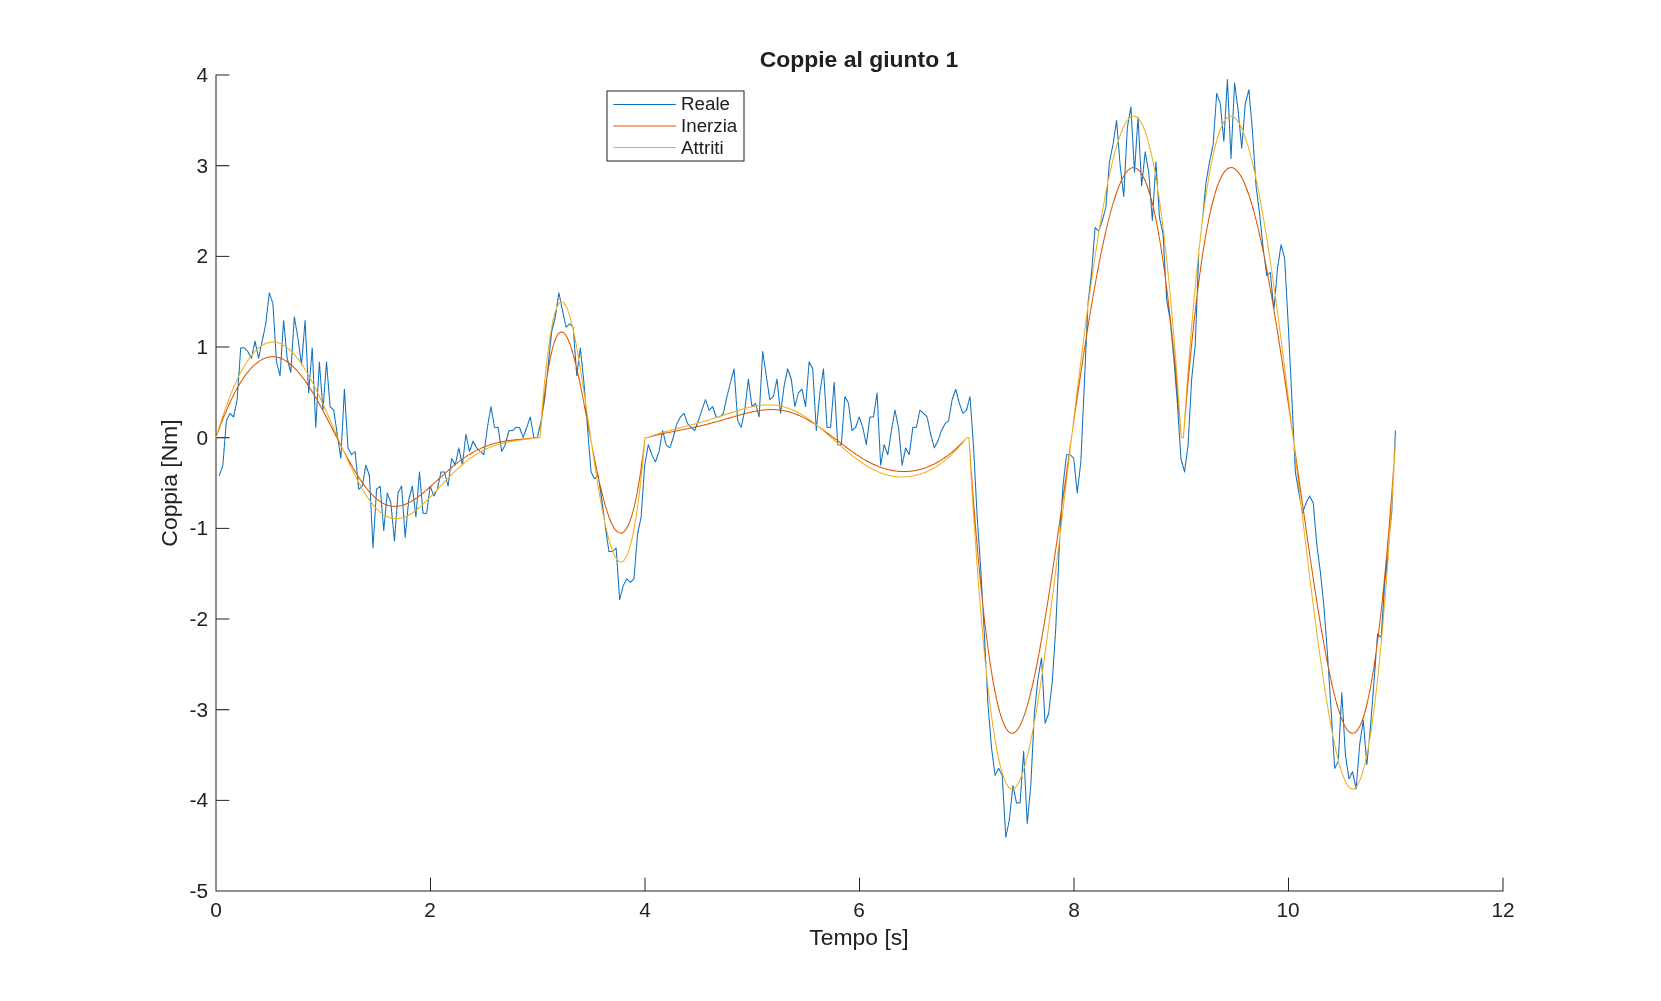
\includegraphics[width=\textwidth]{figure_tesi/coppie_1.png}
		\caption{Giunto 1}
		\label{fig:coppie1}
	\end{subfigure}
	\hfill
	\begin{subfigure}[hbtp]{0.48\textwidth}
		\centering
		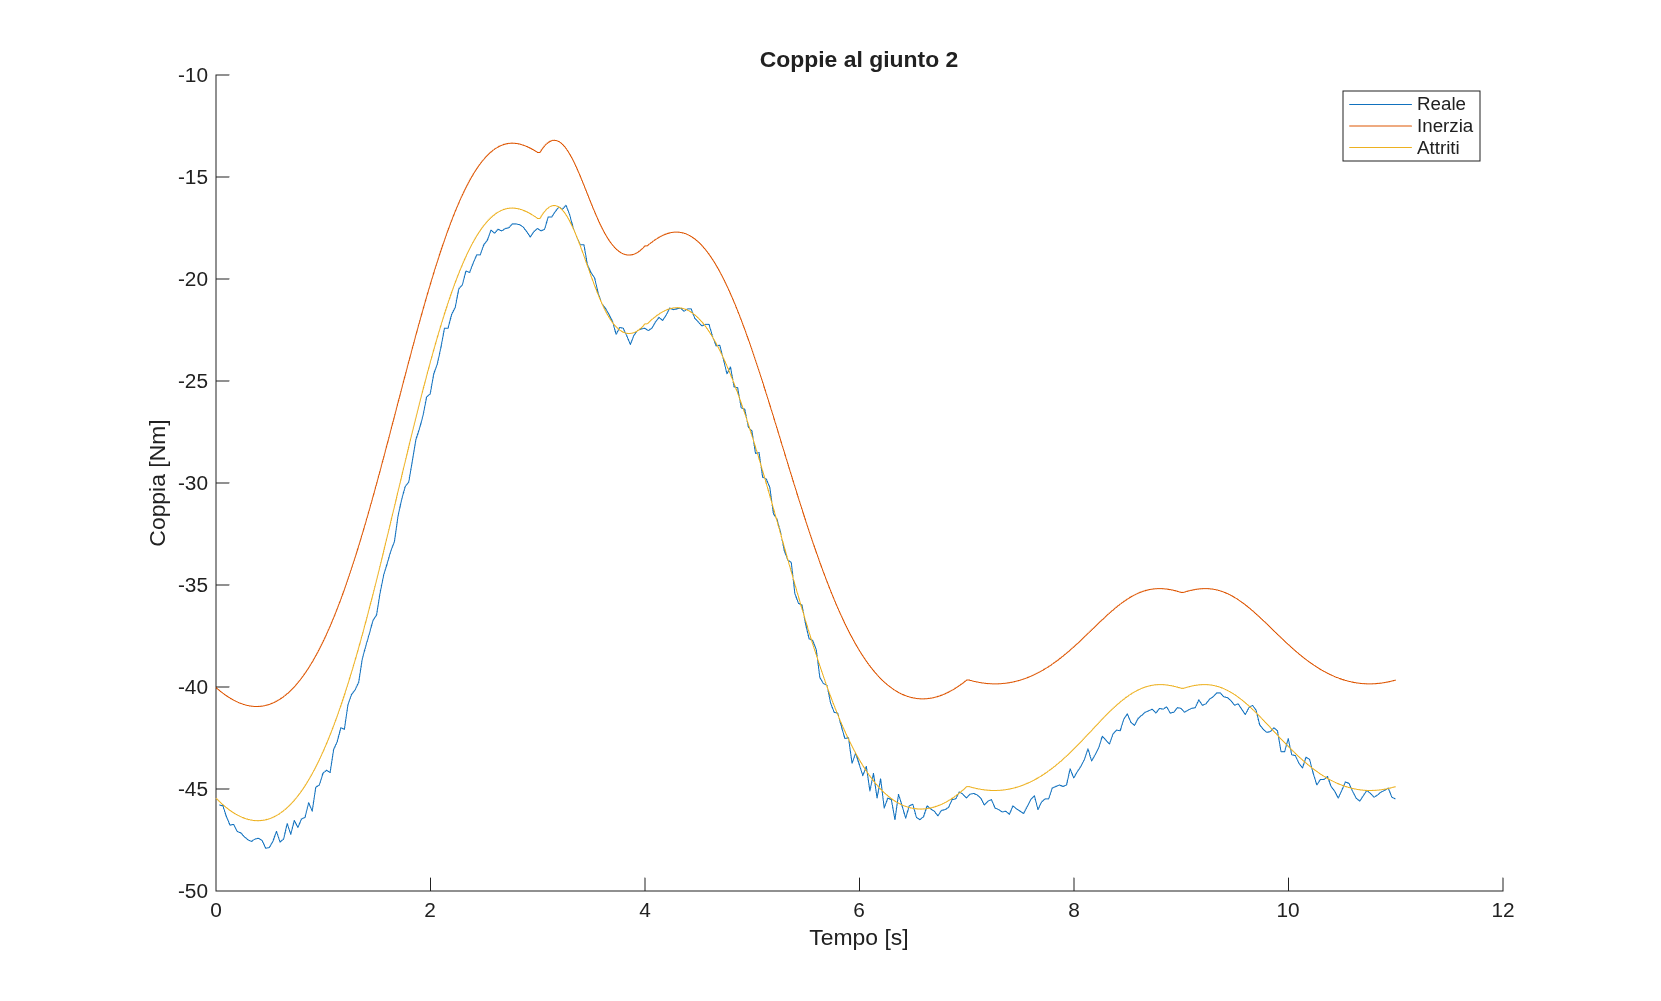
\includegraphics[width=\textwidth]{figure_tesi/coppie_2.png}
		\caption{Giunto 2}
		\label{fig:coppie2}
	\end{subfigure}

	\vspace{0.4cm}
	
	\begin{subfigure}[hbtp]{0.48\textwidth}
		\centering
		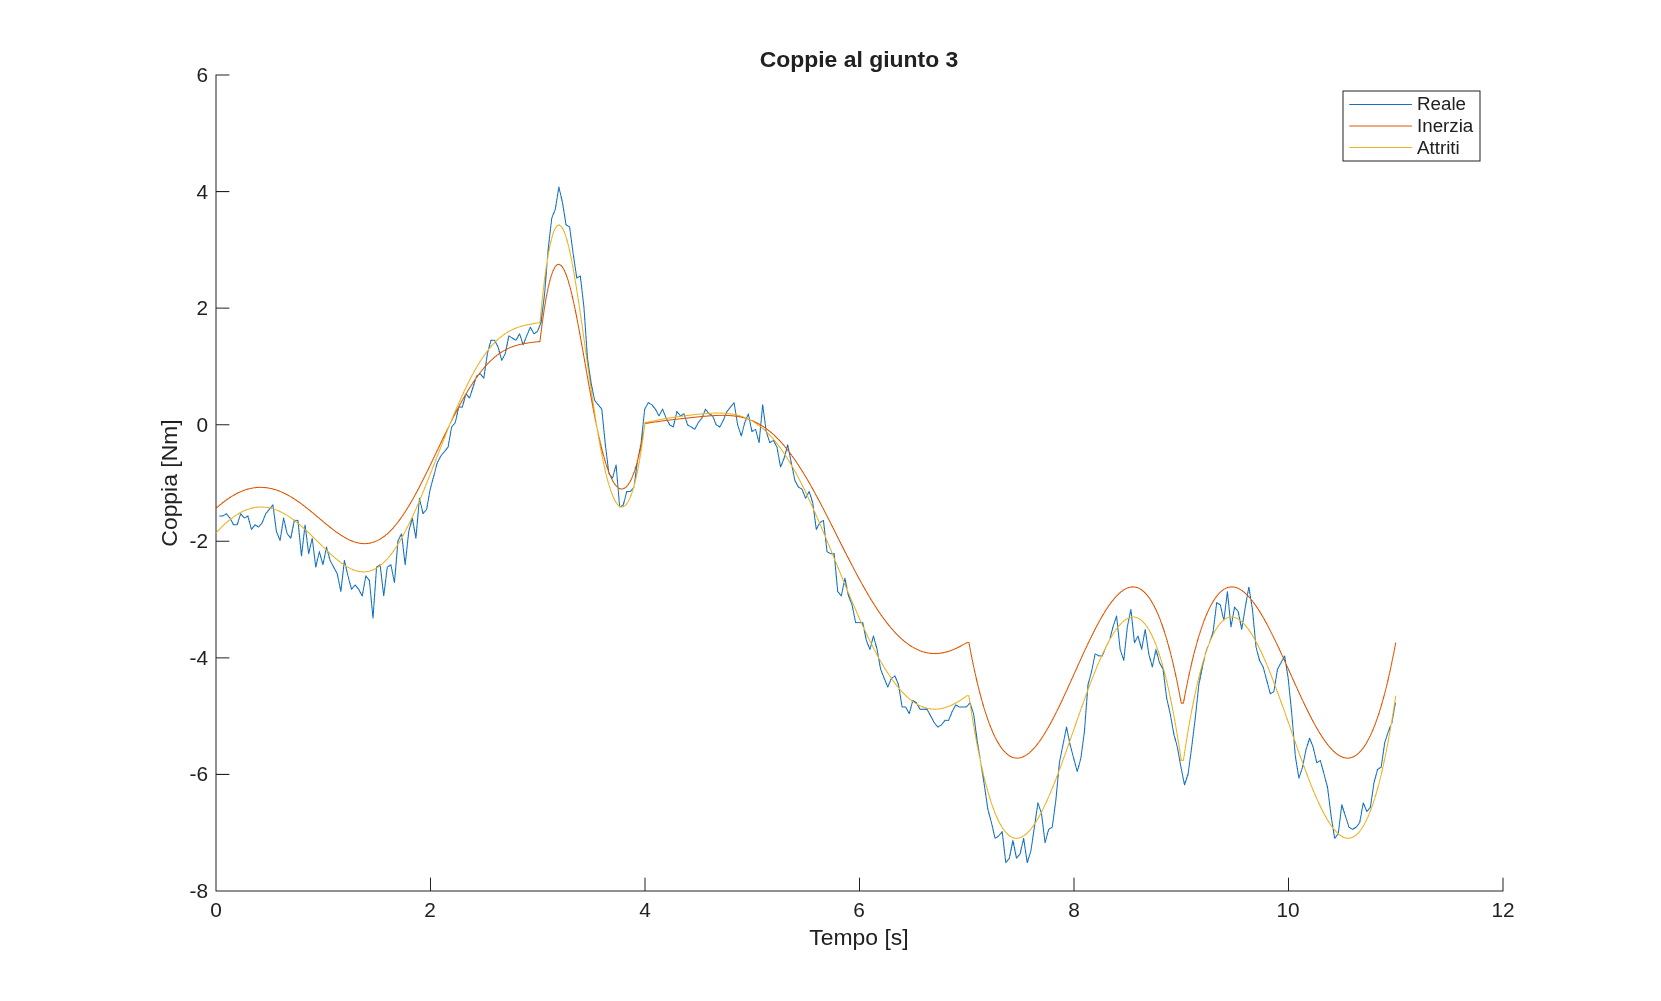
\includegraphics[width=\textwidth]{figure_tesi/coppie_3.png}
		\caption{Giunto 3}
		\label{fig:coppie3}
	\end{subfigure}
	\begin{subfigure}[hbtp]{0.48\textwidth}
		\centering
		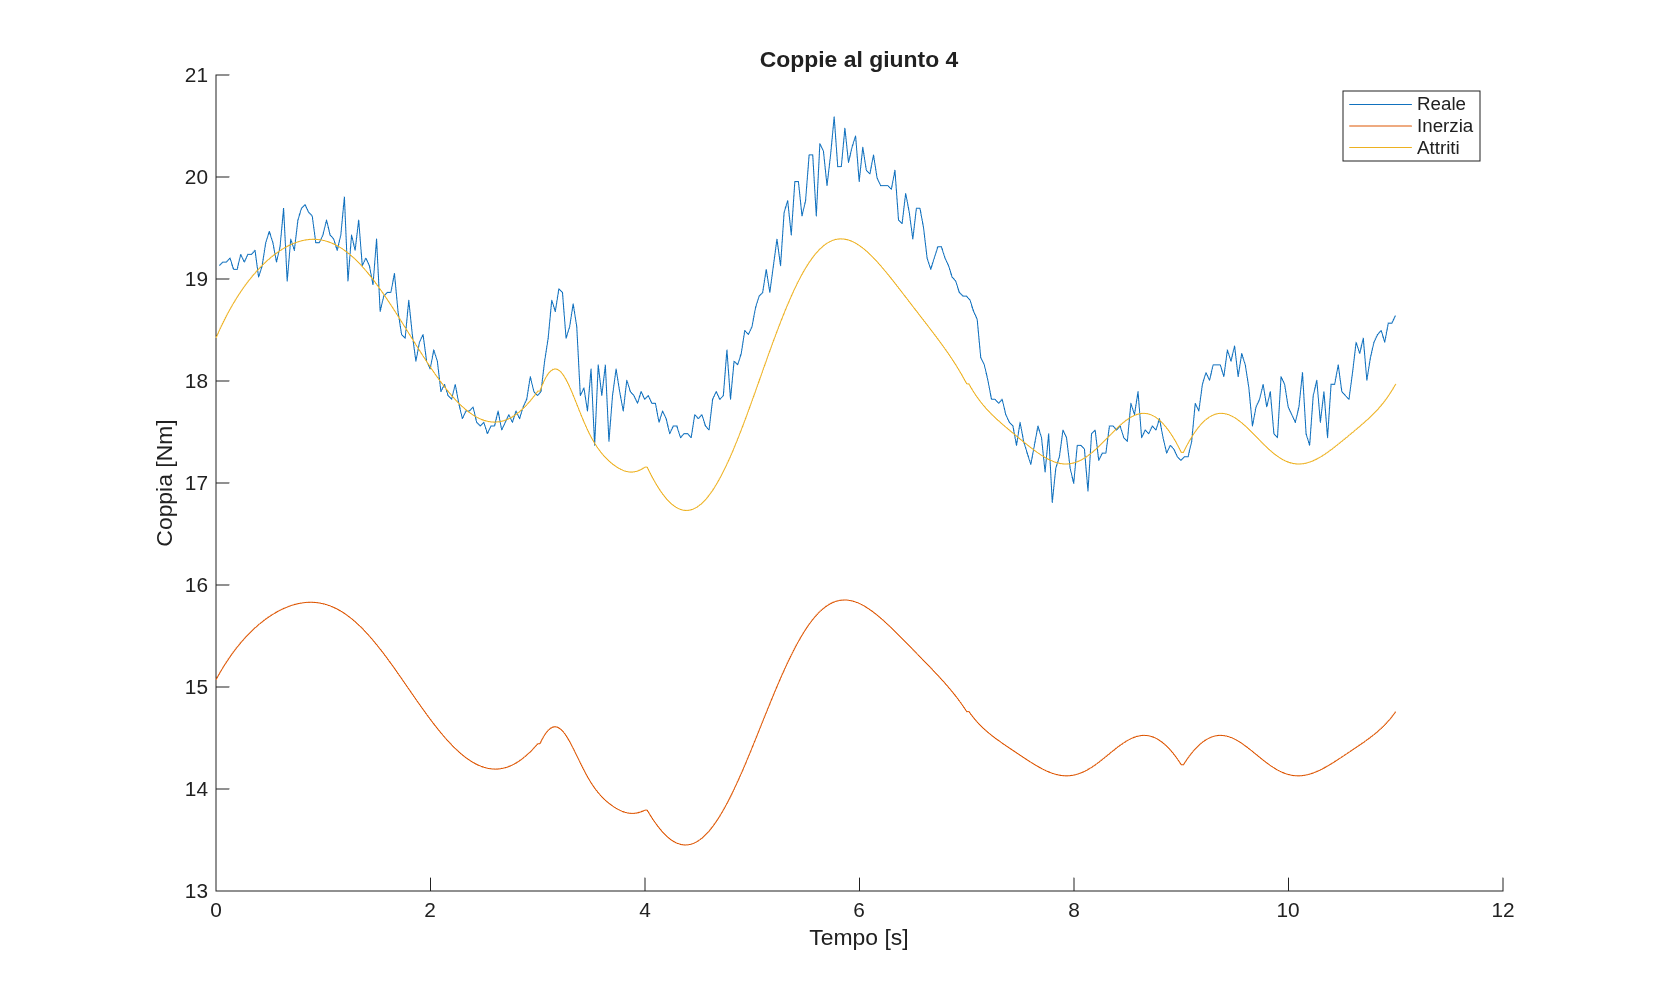
\includegraphics[width=\textwidth]{figure_tesi/coppie_4.png}
		\caption{Giunto 4}
		\label{fig:coppie4}
	\end{subfigure}

	\vspace{0.4cm}
	
	\begin{subfigure}[hbtp]{0.48\textwidth}
		\centering
		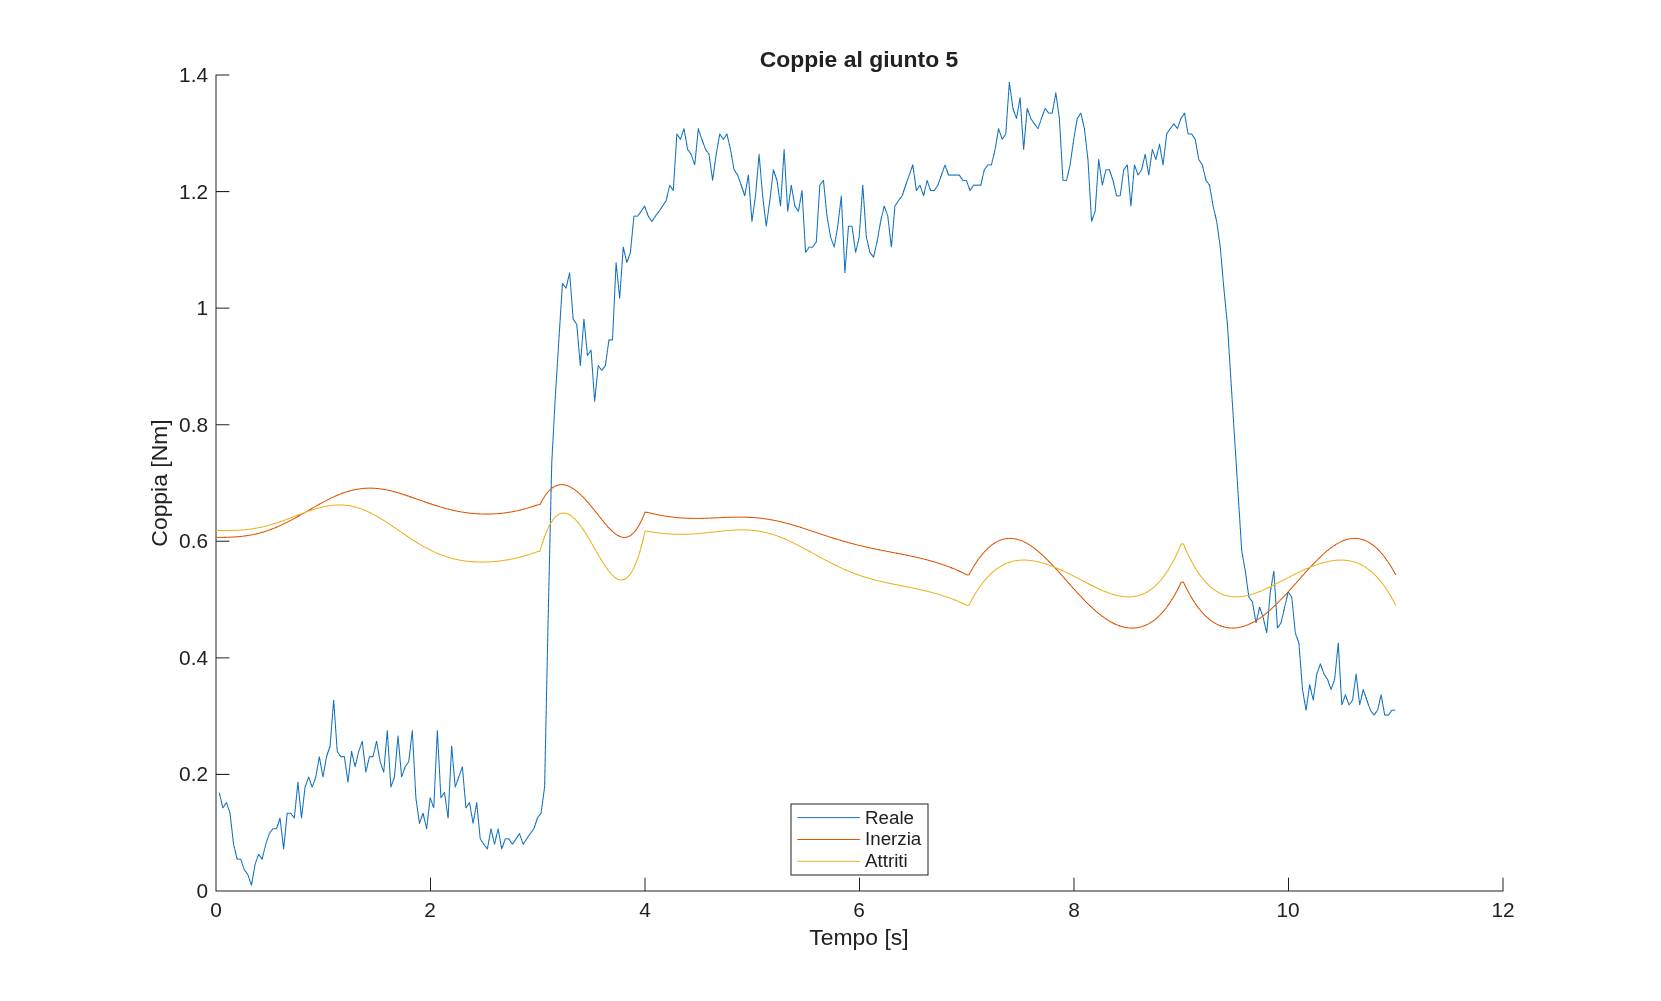
\includegraphics[width=\textwidth]{figure_tesi/coppie_5.png}
		\caption{Giunto 5}
		\label{fig:coppie5}
	\end{subfigure}
	\hfill
	\begin{subfigure}[hbtp]{0.48\textwidth}
		\centering
		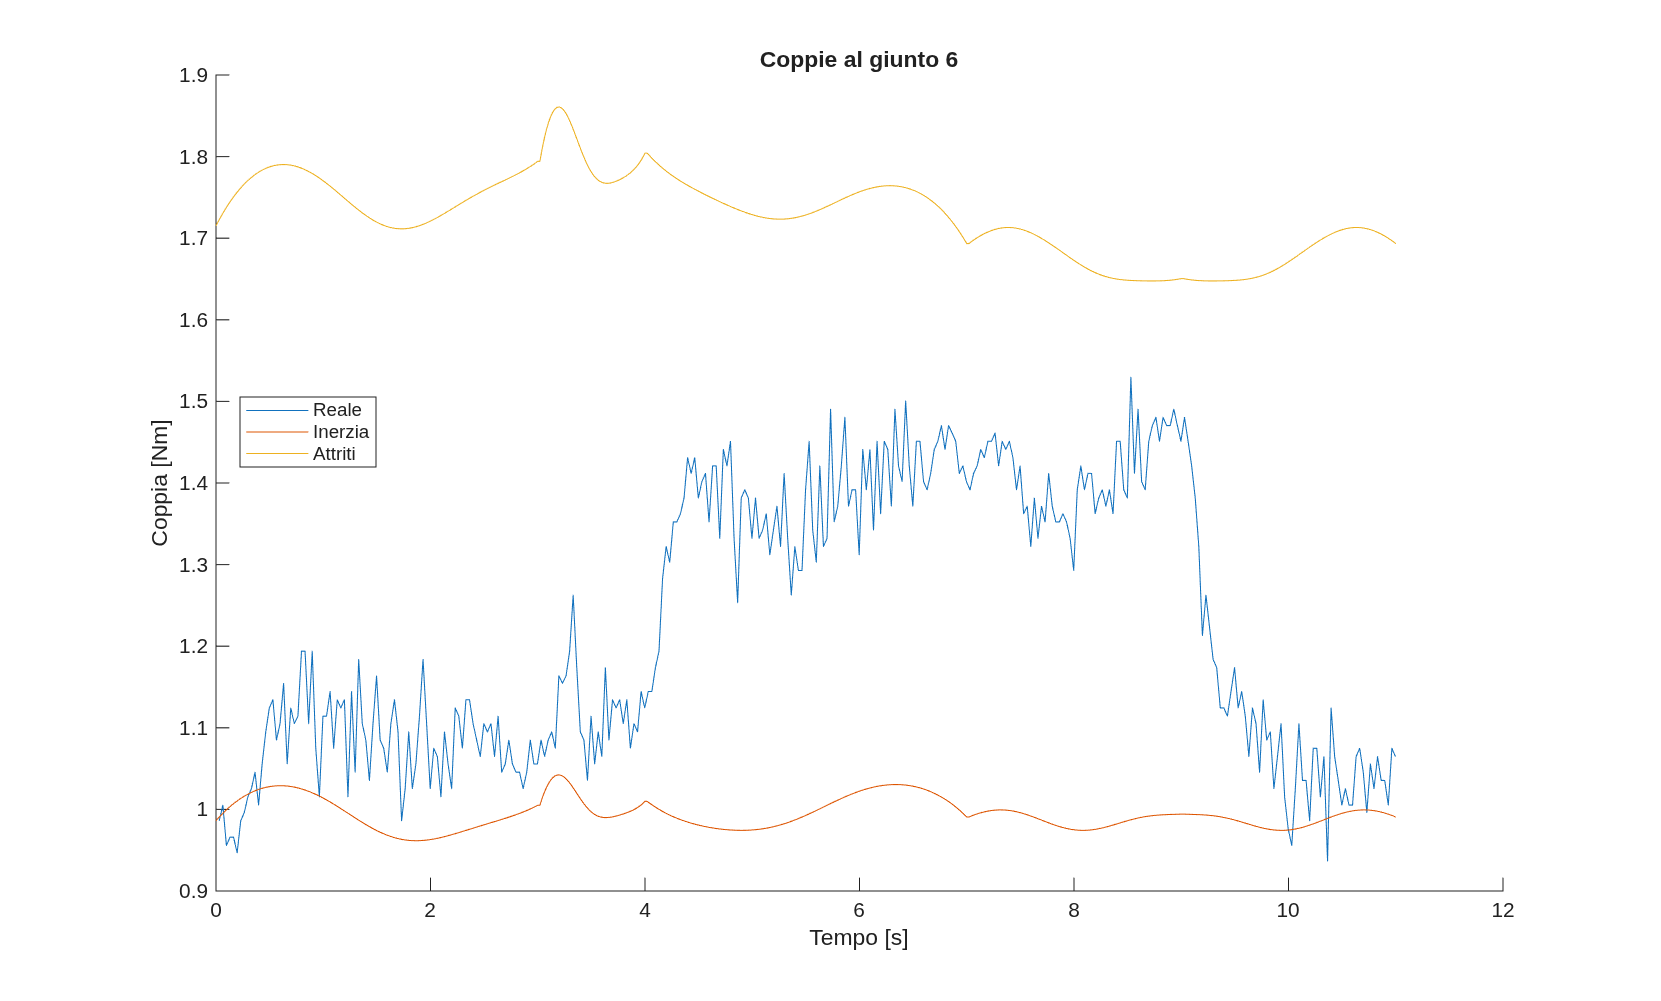
\includegraphics[width=\textwidth]{figure_tesi/coppie_6.png}
		\caption{Giunto 6}
		\label{fig:coppie6}
	\end{subfigure}

	\vspace{0.4cm}
	\begin{subfigure}[hbtp]{0.48\textwidth}
		\centering
		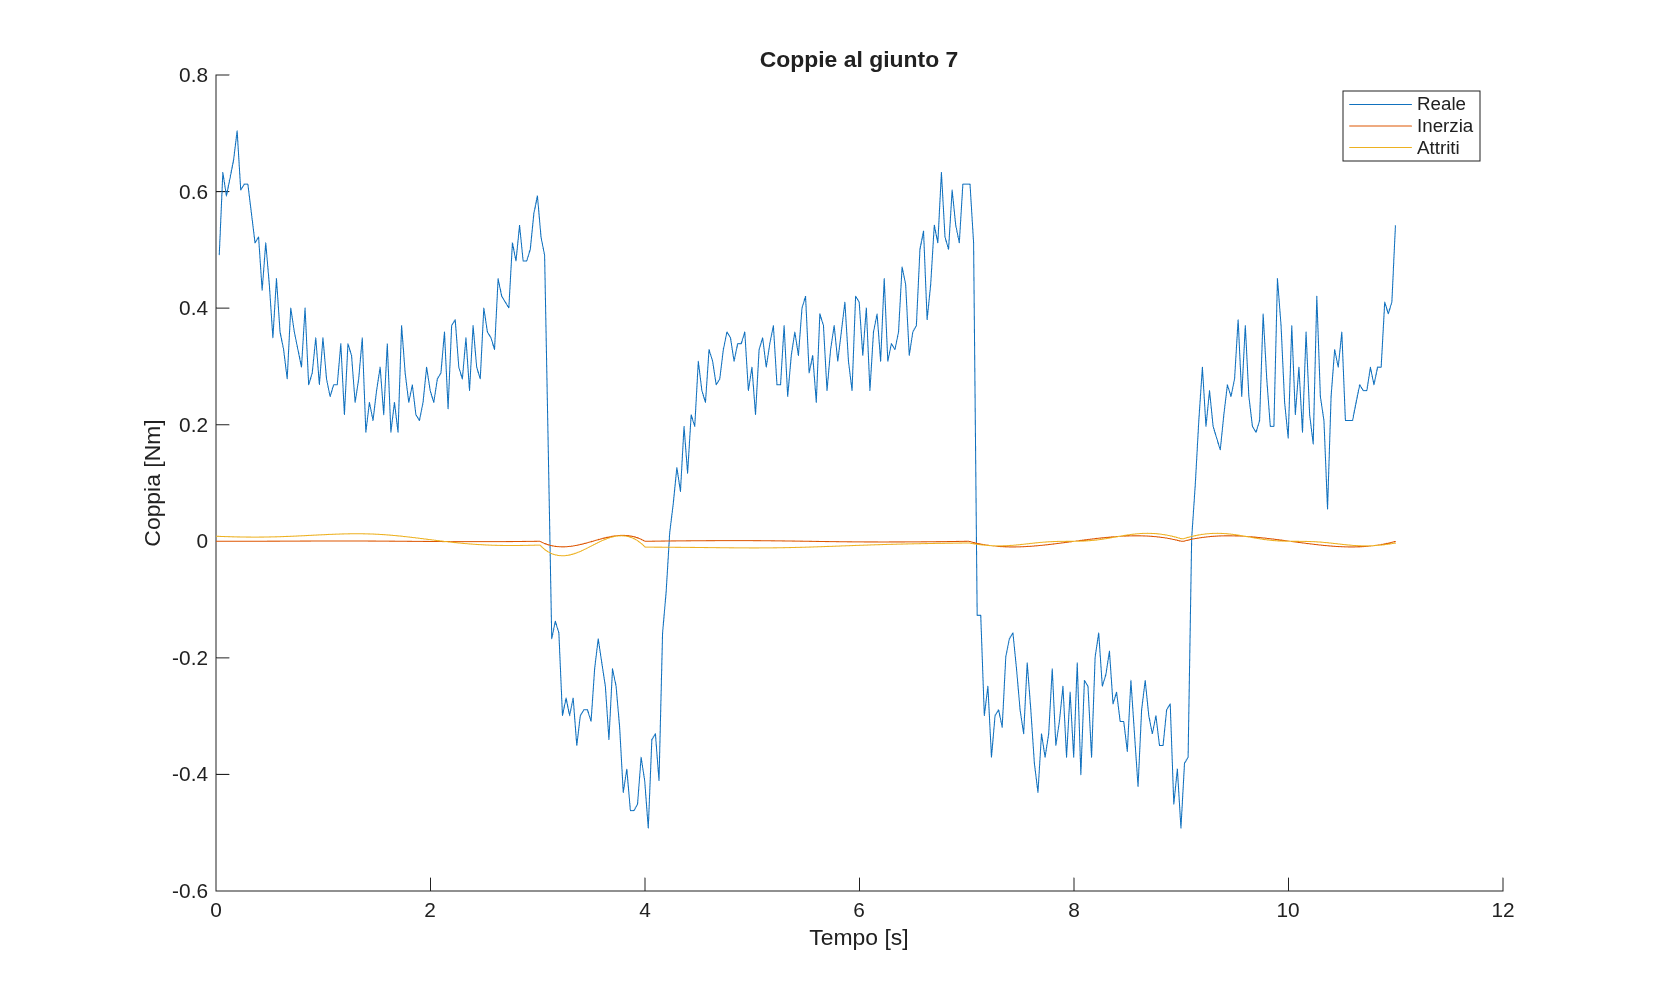
\includegraphics[width=\textwidth]{figure_tesi/coppie_7.png}
		\caption{Giunto 7}
		\label{fig:coppie7}
	\end{subfigure}
	

	\caption{Confronto tra le coppie reali misurate ai giunti e le coppie stimate tramite il modello dinamico in Pinocchio.}
	\label{fig:confronto_coppie}
	
\end{figure}

\subsection{Ambiente di simulazione}

Per consentire una rapida validazione del codice ed evitare rischi legati a malfunzionamenti dell'haardware reale, è stata sviluppata una libreria di simulazione in C++ che rispecchia l'interfaccia di \texttt{libfranka}.

In particolare il metodo \texttt{robot.control(...)} è stato implementato adottando un modello di controllo ideale, in cui il robot insegue i comandi ricevuti in modo perfetto. Il Listato~\ref{lst:sim_control} mostra l'implementazione del loop di controllo principale a 1kHz.

\begin{lstlisting}[language=C++, caption={Implementazione del controllo ideale nell'ambiente di simulazione.}, label={lst:sim_control}]
	// Mirror robot.control(), runs callback at 1kHz
	void control(std::function<JointPositions(const RobotState&, Duration)> callback) {
		Duration period;
		
		while (true) {
			JointPositions cmd = callback(state_, period);
			
			// Update simulated state, assume robot perfectly tracks commands
			for (int j = 0; j < 7; ++j) {
			state_.dq[j]  = (cmd.q[j] - state_.q[j]) / period.toSec();
			state_.ddq_d[j] = (state_.dq[j] - prev_dq_[j]) / period.toSec();
			prev_dq_[j] = state_.dq[j];
			state_.q[j] = cmd.q[j];
			state_.q_d[j] = cmd.q[j];
			}
			
			if (cmd.motion_finished) break;
			
			std::this_thread::sleep_for(std::chrono::milliseconds(1));
		}
	}
\end{lstlisting}

L'architettura della libreria si ispira al lavoro di Oliva et al.~\cite{oliva2022frankasim}. Trattandosi di un simulatore cinematico privo di un modello dinamico o fisico dettagliato del manipolatore, l'ambiente virtuale non contempla gli attriti, i goichi meccanici e le non idealità proprie del robot reale (trattate in dettaglio nella Sezione~\ref{subsec:controllo_posizione}).

\section{Sistema di visione e playback dello scheletro}
L'acquisizione visiva della scena viene effettuata tramite una telecamera di profondità Intel Realsense D435. Il dispositivo calcola la mappa di profondità direttamente a bordo tramite l'ASIC dedicato, sgravando l'unità di calcolo ospite da tale carico computazionale \cite{tadic2019application}.

A partire dalle immagini acquisite, la posa dello scheletro umano viene stimata mediante il framework MediaPipe. I punti salienti (\textit{keypoints}) della struttura corporea estratti vengono successivamente salvati su file di testo.

La fase di playback dello scheletro registrato si avvale della libreria ZeroMQ \cite{hintjens2013zeromq}, strutturata secondo un paradigma di comunicazione monodirezionale di tipo \textit{Publisher-Subscriber}. Per garantire il rispetto dei vincoli temporali del ciclo di controllo a 1kHz, l'architettura software impiega due thread distinti:
\begin{itemize}
	\item \textbf{Nodo Python (\textit{Publisher}):} trasmette le coordinate dei punti salienti dello scheletro stimato;
	\item \textbf{Nodo C++ (\textit{Subscriber}):} riceve i dati in streaming e li memorizza in un vettore condiviso (\textit{Skeleton}) accessibile dal programma di controllo principale.
\end{itemize}


\section{Primo metodo: frenata morbida}
\label{sec:frenata}

Come visto in Sezione~\ref{sec:primo_approccio}, è necessario risolvere un problema di ottimizzazione vincolata. Per fare ciò si è deciso di utilizzare il framework open-source \textit{CasADi}~\cite{Andersson2018}.

\subsection{Ottimizzazione tramite CasADi}
\textit{CasADi} è uno strumento software ad alte prestazioni sviluppato per l'ottimizzazione numerica, con particolare attenzione all'ottimizzazione vincolata non lineare (NLP) e al controllo ottimale. È scritto in C++ con interfacce per Python e MATLAB, rendendolo estremamente versatile sia in fase di prototipazione che di implementazione in sistemi embedded o ad alte prestazioni.

Il punto di forza di CasADi risiede nella sua struttura simbolica basata sui grafi di espressione (\textit{expression graphs}). Ciò consente di eseguire la Differenziazione Algoritmica (AD) sia in modalità diretta (\textit{forward mode}) sia inversa (\textit{reverse mode}). In questo modo, derivate prime (gradienti, Jacobiane) e derivate seconde (Hessiane) vengono calcolate con accuratezza pari alla precisione della macchina, evitando le imprecisioni numeriche della differenziazione alle differenze finite e l'esplosione della complessità del calcolo simbolico classico.

Un generico problema di ottimizzazione non lineare (NLP) risolto da CasADi viene formulato nella seguente forma standard:
\begin{equation}
\begin{aligned}
\min_{x} \quad & f(x) \
\textrm{s.t.} \quad & x_{lb} \le x \le x_{ub} \
& g_{lb} \le g(x) \le g_{ub}
\end{aligned}
\end{equation}
dove $x \in \mathbb{R}^n$ rappresenta il vettore delle variabili decisionali, $f(x): \mathbb{R}^n \to \mathbb{R}$ è la funzione obiettivo (cost function), $x_{lb}$ e $x_{ub}$ sono i limiti inferiori e superiori sulle variabili (box constraints), mentre $g(x): \mathbb{R}^n \to \mathbb{R}^m$ rappresenta il vettore delle funzioni di vincolo non lineare bounded da $g_{lb}$ e $g_{ub}$.

Per la risoluzione del problema, CasADi mette a disposizione l'interfaccia ad alto livello \texttt{casadi::nlpsol}. Questa interfaccia accetta un dizionario \texttt{nlp} contenente la definizione simbolica di $x$, $f(x)$ e $g(x)$, unita alla specifica del solutore numerico sottostante (come ad esempio \textit{IPOPT}, \textit{SNOPT} o \textit{KNITRO}).

\subsubsection{Esempio di risoluzione NLP in C++}
Di seguito viene mostrato un esempio applicativo in C++ per la risoluzione di un problema di ottimizzazione non lineare limitato e vincolato Eq.~\ref{eq:nlp} tramite il solutore IPOPT integrato in CasADi:

\begin{equation}
\min_{x_0, x_1} \quad x_0^2 + (x_1 - 1)^2 \quad \textrm{s.t.} \quad x_0 + x_1 = 2, \quad x_0 \ge 0, ; x_1 \ge 0
\label{eq:nlp}
\end{equation}

\begin{lstlisting}[language=C++]
#include <casadi/casadi.hpp>
#include

using namespace casadi;

int main() {
// 1. Definizione delle variabili simboliche (SX o MX)
SX x = SX::sym("x", 2); // Vettore di 2 variabili decisionali (x0, x1)
// 2. Definizione della funzione costo f(x) e dei vincoli g(x)
SX f = pow(x(0), 2) + pow(x(1) - 1, 2);
SX g = x(0) + x(1);

// 3. Creazione del dizionario NLP per CasADi
MXDict nlp = {
{"x", x},
{"f", f},
{"g", g}
};

// 4. Inizializzazione del solutore (es. IPOPT)
// E possibile passare opzioni aggiuntive come secondo argomento (Dict)
Function solver = nlpsol("solver", "ipopt", nlp);

// 5. Impostazione dei limiti numerici sui vincoli e sulle variabili
DNDict args;
args["x0"]  = std::vector<double>{0.0, 0.0};  // Punto di partenza (Initial guess)

// Bounds sulle variabili x (x >= 0)
args["lbx"] = std::vector<double>{0.0, 0.0};  
args["ubx"] = std::vector<double>{inf, inf};  

// Bounds sul vincolo g(x) = 2 -> lbg = ubg = 2
args["lbg"] = std::vector<double>{2.0};
args["ubg"] = std::vector<double>{2.0};

// 6. Risoluzione del problema
DNDict res = solver(args);

// 7. Estrazione dei risultati
std::vector<double> x_opt = std::vector<double>(res["x"]);
std::cout << "Soluzione ottimale x: [" << x_opt[0] << ", " << x_opt[1] << "]" << std::endl;
std::cout << "Valore minimo costo: " << double(res["f"]) << std::endl;

return 0;

}
\end{lstlisting}

\subsection{Rilevamento di una potenziale collisione}
La libreria \textit{CasADi} descritta nella sezione precedente viene utilizzata per risolvere il problema di ottimizzazione definito nella Sezione~\ref{subsec:optimization_problem}, vincolato ai limiti di posizione, velocità, accelerazione e coppia dei giunti del robot:
\begin{equation}
\min_{T_{\text{stop}}} \quad w_0 T_{\text{stop}} + w_1 \left|T_{\text{stop}}-T_{\text{stop,prev}} \right|
\label{eq:costo}
\end{equation}

Per garantire il rispetto dei vincoli temporali e non bloccare l'esecuzione del task nominale, l'architettura software sfrutta due thread dedicati:
\begin{itemize}
	\item \texttt{skeleton\_thread}: gestisce la ricezione e il playback in tempo reale delle posizioni delle articolazioni dello scheletro umano;
	\item \texttt{collision\_checker\_thread}: esegue la risoluzione dell'ottimizzazione in Eq.~\eqref{eq:costo} nell'intervallo $T_{\text{stop}} \in [0.1, 0.4]~\text{s}$ a partire dallo stato corrente del robot letto tramite \textit{libfranka}, integrando il modello cinematico e dinamico fornito da \textit{Pinocchio}.
\end{itemize}

I parametri geometrici, cinematici e numerici adottati nell'implementazione dell'algoritmo sono sintetizzati nella Tabella~\ref{tab:collision_params}.

\begin{table}[htbp]
	\centering
	\caption{Parametri geometrici, cinematici e di configurazione usati dall'algoritmo di rilevamento collisione.}
	\label{tab:collision_params}
	\begin{tabular}{lccc}
		\toprule
		\textbf{Parametro} & \textbf{Simbolo} & \textbf{Valore} & \textbf{Unità di misura} \\
		\midrule
		\multicolumn{4}{l}{\textit{Modello geometrico (Capsule SSL)}} \\
		Raggio capsula 1 robot & $r_{r,1}$ & $0.085$ & \text{m} \\
		Raggio capsula 2 robot & $r_{r,2}$ & $0.085$ & \text{m} \\
		Raggio capsula 3 robot & $r_{r,3}$ & $0.060$ & \text{m} \\
		Raggio capsula 4 robot & $r_{r,4}$ & $0.065$ & \text{m} \\
		Raggio capsule scheletro umano & $r_h$ & $0.05 - 0.16$ & \text{m} \\
		\midrule
		\multicolumn{4}{l}{\textit{Parametri cinematici e tempi}} \\
		Velocità massima stimata umano & $v_{\text{human, max}}$ & $1.60$ & \text{m/s} \\
		Tempo di reazione del sistema & $T_{\text{reaction}}$ & $0.05$ & \text{s} \\
		\midrule
		\multicolumn{4}{l}{\textit{Vincoli e impostazioni ottimizzatore (CasADi)}} \\
		Tempo di stop minimo & $T_{\text{stop, min}}$ & $0.10$ & \text{s} \\
		Tempo di stop massimo & $T_{\text{stop, max}}$ & $0.40$ & \text{s} \\
		Peso termine tempo di stop & $w_0$ & $10^6$ & -- \\
		Peso variazione tempo di stop & $w_1$ & $10^6$ & -- \\
		Numero massimo di iterazioni & $\texttt{max\_iter}$ & $5$ & -- \\
		\bottomrule
	\end{tabular}
\end{table}

Per garantire un approccio cautelativo (worst-case scenario), la velocità massima dell'umano $v_{\text{human, max}}$ è stata impostata a $1.60\,\text{m/s}$, in accordo con le direttive sulle velocità di avvicinamento stabilite dalla norma ISO/TS 15066 per applicazioni collaborative. I raggi delle primitive SSL ($r_r$ e $r_h$) coprono l'ingombro effettivo dei link del robot Franka Emika Panda e dei segmenti corporei dell'operatore.

A partire dal tempo $T_{\text{stop}}$ ottimizzato ad ogni ciclo, la distanza di separazione minima di sicurezza $d_{\text{safe}}$ considerata nell'algoritmo viene calcolata dinamicamente come:
\begin{equation}
d_{\text{safe}} = v_{\text{human, max}} \cdot \left( T_{\text{reaction}} + T_{\text{stop}} \right)
\label{eq:d_safe}
\end{equation}
Se la distanza tra i volumi SSL del robot e dell'umano risulta inferiore a $d_{\text{safe}}$, viene rilevata una potenziale collisione e attivata la traiettoria di arresto arresto entro il tempo $T_{\text{stop}}$.

\subsection{Esecuzione del Task}
L'applicazione di test sviluppata per la validazione delle strategie di sicurezza nella collaborazione uomo-robot (HRC) consiste in un task sequenziale di \textit{pick and place}. Dal punto di vista software, la logica di controllo in C++ è stata architettata ed eseguita come una macchina a stati finiti (FSM, \textit{Finite State Machine}), garantendo una gestione deterministica delle transizioni tra la traiettoria nominale e le manovre di arresto di sicurezza.

\subsubsection{Architettura Software e Flusso di Esecuzione}
A livello concettuale, la macchina a stati si fonda su due macro-stati operativi principali:
\begin{itemize}
	\item \texttt{RUNNING}: il manipolatore insegue la traiettoria nominale pianificata nello spazio dei giunti o cartesiano. Al raggiungimento di ciascun \textit{waypoint} intermedio, l'algoritmo provvede al calcolo e all'interpolazione del segmento di traiettoria successivo.
	\item \texttt{STOPPING}: innescato dal rilevamento di una condizione di potenziale pericolo o dalla violazione delle distanze di sicurezza, questo stato forza l'esecuzione di una traiettoria di arresto a tempo ottimo (\textit{time-optimal stopping trajectory}). Al termine della decelerazione, il robot viene mantenuto in uno stato di arresto temporaneo per un intervallo di tempo prefissato, durante il quale il sistema calcola la nuova traiettoria di ripartenza in modo da garantire un rientro fluido e privo di urti (\textit{jerk-free}) sulla traiettoria nominale.
\end{itemize}

Dal punto di vista dell'implementazione software, la FSM non è strutturata all'interno di un unico blocco condizionale, ma si articola attraverso una gerarchia di funzioni che separano la \textit{pianificazione di alto livello} dal \textit{loop di controllo ad alta frequenza} (\SI{1}{\kHz}). Il flusso operativo segue una logica ciclica suddivisa nei seguenti passi:

\begin{enumerate}
	\item \textbf{Pianificazione e Inizializzazione (Alto Livello):} La funzione principale di gestione (\textit{executeTask}) configura i dati di input, calcola analiticamente i segmenti della traiettoria desiderata e invoca l'esecutore di movimento ad alta frequenza.
	\item \textbf{Esecuzione Real-Time (\SI{1}{\kHz}):} La funzione di controllo a \SI{1}{\kHz} (\textit{executeTrajectory}, implementata tramite costrutto \textit{lambda} in C++) esegue l'inseguimento della traiettoria generata. Il loop controlla continuamente le condizioni di terminazione o di interruzione:
	\begin{itemize}
		\item Se il robot raggiunge la configurazione finale nominale, la funzione solleva la condizione di fine movimento (\texttt{franka::MotionFinished}) e restituisce il controllo al livello superiore.
		\item Se si verifica una condizione di stop per sicurezza, il sistema commuta nello stato \texttt{STOPPING}, porta il robot all'arresto in tempo ottimo e termina l'esecuzione del ciclo ad alta frequenza.
	\end{itemize}
	\item \textbf{Fase di Stasi e Ri-pianificazione (\textit{Re-planning State}):} Al rientro dal loop real-time, il programma entra in uno stato transitorio di stasi. In questo intervallo il robot rimane fermo in posizione di sicurezza, mentre il thread di alto livello valuta la nuova configurazione e ricalcola la traiettoria di rientro prima di richiamare nuovamente il ciclo di controllo a \SI{1}{\kHz}.
\end{enumerate}

La Figura~\ref{fig:architettura_macchina_stati} illustra lo schema concettuale di tale architettura. Come si può notare, il sistema commuta in modo deterministico tra il livello di pianificazione ad alto livello e il loop di controllo ad alta frequenza. Quando la traiettoria viene completata o interrotta nello stato \texttt{STOPPING}, la restituzione dell'oggetto \texttt{franka::MotionFinished} riporta l'esecuzione allo stato di stasi ad alto livello, consentendo il ricalcolo sicuro della nuova traiettoria senza saturare il thread real-time.

\begin{figure}[htbp]
	\centering
	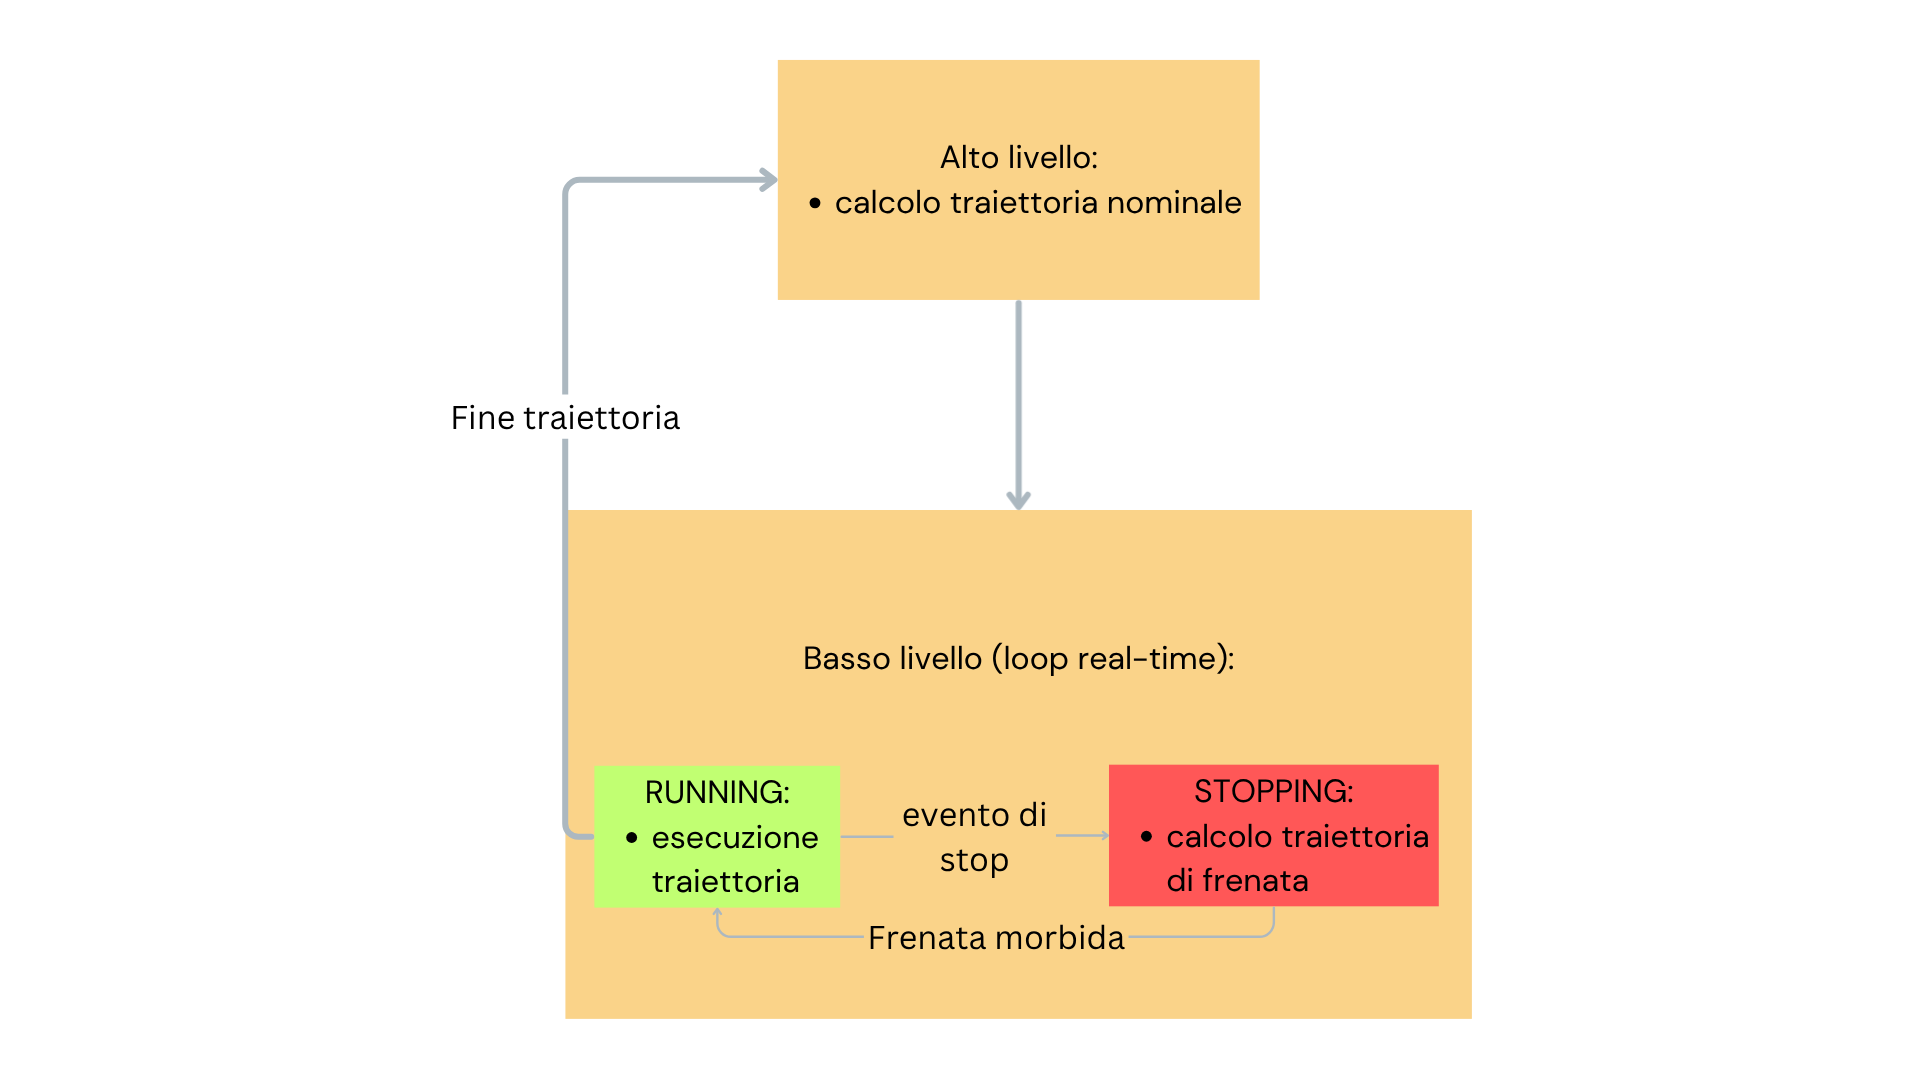
\includegraphics[width=0.8\textwidth]{figure_tesi/schema_controllo.png}
	\label{fig:architettura_macchina_stati}
	\caption{Architettura software del sistema di controllo. L'alto livello gestisce la pianificazione offline e la ri-pianificazione delle traiettorie, mentre il basso livello esegue il loop di controllo ad alta frequenza ($1\text{ kHz}$) alternando deterministicamente gli stati di \texttt{RUNNING} e \texttt{STOPPING}.}
\end{figure}


Nel seguito vengono analizzate ed elaborate due strategie di controllo implementate tramite le API di basso livello di \texttt{libfranka}: il controllo in posizione e il controllo in coppia.

\subsubsection{Controllo di Posizione dei Giunti}
\label{subsec:controllo_posizione}
In prima istanza, la movimentazione del robot è stata implementata sfruttando l'interfaccia di controllo in posizione fornita da \texttt{libfranka}, mediante il metodo generico:
\begin{lstlisting}[language=C++]
robot.control([&](const franka::RobotState& state, franka::Duration period) 
-> franka::JointPositions { ... });
\end{lstlisting}

Attraverso questo approccio, la funzione \textit{lambda} viene eseguita all'interno del loop di controllo ad alta frequenza ($1\text{ kHz}$) e restituisce al controllore interno del manipolatore i valori obiettivo per le posizioni dei giunti ($\mathbf{q}_d$). 

Sebbene questo approccio abbia mostrato prestazioni soddisfacenti nell'ambiente di simulazione, l'applicazione sul robot reale ha evidenziato criticità applicative. In particolare, si sono riscontrate discontinuità nel profilo delle velocità misurate ai giunti, accompagnate da sollecitazioni meccaniche udibili e vibrazioni indesiderate sulla struttura del manipolatore. Tale fenomeno è riconducibile al fatto che l'invio diretto di posizioni discrete, se non accuratamente filtrato a livello di \textit{jerk}, può generare derivate prime e seconde non continue, attivando i filtri di protezione interni del robot o causandone un comportamento a scatti.

Per la gestione dell'arresto definitivo o del completamento del movimento, l'uscita dal ciclo di controllo viene notificata al sistema restituendo l'oggetto di terminazione con lo stato finale desiderato, mantenendo la posizione corrente di riferimento:
\begin{lstlisting}[language=C++]
return franka::MotionFinished(franka::JointPositions(state.q_d));
\end{lstlisting}

\subsubsection{Controllo di Coppia e Controllo di Impedenza}
\label{subsec:controllo_coppia}
Per risolvere le discontinuità nei profili di velocità e garantire un'interazione intrinsecamente sicura durante l'esecuzione del task, si è scelto di implementare uno schema di controllo di coppia (\textit{torque control}) in C++. L'interfaccia sfrutta il seguente metodo:
\begin{lstlisting}[language=C++]
robot.control([&](const franka::RobotState& state, franka::Duration period) 
-> franka::Torques { ... });
\end{lstlisting}

Per garantire un inseguimento preciso e reattivo della traiettoria, è stata adottata una legge di controllo a coppia calcolata (\textit{Computed Torque Control}), che unisce un'azione di \textit{feedforward} (basata sul modello dinamico inverso del robot) ad un'azione di \textit{feedback} proporzionale-derivativa (PD) per regolare l'impedenza ai giunti. 

Matematicamente, la coppia desiderata $\boldsymbol{\tau}_d \in \mathbb{R}^7$ da applicare ai giunti è calcolata come:
\begin{equation}
\boldsymbol{\tau}_d = \mathbf{M}(\mathbf{q}) \ddot{\mathbf{q}}_d + \mathbf{C}(\mathbf{q}, \dot{\mathbf{q}}) + \mathbf{K}_p (\mathbf{q}_d - \mathbf{q}) + \mathbf{K}_d (\dot{\mathbf{q}}_d - \dot{\mathbf{q}})
\end{equation}
dove:
\begin{itemize}
	\item $\mathbf{M}(\mathbf{q}) \in \mathbb{R}^{7 \times 7}$ è la matrice di inerzia dipendente dalla configurazione attuale $\mathbf{q}$;
	\item $\mathbf{C}(\mathbf{q}, \dot{\mathbf{q}}) \in \mathbb{R}^7$ è il vettore che raggruppa gli effetti di Coriolis e le forze centrifughe;
	\item $\mathbf{q}_d, \dot{\mathbf{q}}_d, \ddot{\mathbf{q}}_d \in \mathbb{R}^7$ sono rispettivamente posizione, velocità ed accelerazione desiderate ai giunti, calcolate dal generatore di traiettoria;
	\item $\mathbf{K}_p, \mathbf{K}_d \in \mathbb{R}^{7 \times 7}$ sono le matrici diagonali dei guadagni (rispettivamente di rigidezza e smorzamento) del controllore di impedenza.
\end{itemize}

\textit{Nota: Il vettore della gravità $\mathbf{g}(\mathbf{q})$ non compare esplicitamente nella legge di controllo, poiché l'interfaccia \texttt{libfranka} provvede, di default, a sommare la compensazione di gravità interna ai comandi di coppia forniti dall'utente.}

A livello software, l'implementazione nel loop di controllo a $1\text{ kHz}$ necessita della classe \texttt{franka::Model} per recuperare i parametri dinamici aggiornati. Poiché le API di \texttt{libfranka} restituiscono questi dati sotto forma di \texttt{std::array}, si è fatto ricorso alla libreria \texttt{Eigen} e in particolare alla classe \texttt{Eigen::Map}, che permette di proiettare gli array in matrici e vettori senza allocare nuova memoria, ottimizzando così i tempi di calcolo \textit{real-time}:

\begin{lstlisting}[language=C++]
// Acquisizione dei termini dinamici dal modello di libfranka
std::array<double, 49> mass_array = model.mass(state);
std::array<double, 7> coriolis_array = model.coriolis(state);

// Mappatura (zero-copy) degli array in strutture dati Eigen
Eigen::Map<Eigen::Matrix<double, 7, 7>> M(mass_array.data());
Eigen::Map<Eigen::Matrix<double, 7, 1>> C(coriolis_array.data());
Eigen::Map<Eigen::Matrix<double, 7, 1>> q(state.q.data());
Eigen::Map<Eigen::Matrix<double, 7, 1>> dq(state.dq.data());

// Calcolo degli errori di inseguimento (feedback)
Eigen::Matrix<double, 7, 1> error = q_d - q;
Eigen::Matrix<double, 7, 1> derror = dq_d - dq;

// Legge di controllo a coppia calcolata
Eigen::Matrix<double, 7, 1> tau_d;
tau_d = M * ddq_d + C + K_p * error + K_d * derror;

// Invio del comando al manipolatore
std::array<double, 7> tau_d_array;
Eigen::VectorXd::Map(&tau_d_array[0], 7) = tau_d;
return tau_d_array;
\end{lstlisting}

L'adozione di questo schema ha permesso non solo di eliminare le discontinuità e il rumore causati dal controllo di posizione, ma anche di conformare il comportamento dinamico del robot in caso di contatto, un requisito fondamentale per le applicazioni di robotica collaborativa.

\section{Secondo approccio: capsule \textit{soft}}

L'architettura del controllore si basa su una macchina a stati finiti (FSM) analoga a quella presentata nella sezione precedente. La differenza fondamentale risiede nello stato di \textit{RUNNING}, che integra un modulo di verifica per le interazioni con le capsule \textit{soft} esterne per la generazione delle corrispondenti forze repulsive.

Quando una capsula associata all'operatore entra in contatto con una capsula \textit{soft} del robot, il sistema calcola una forza virtuale repulsiva. L'entità di tale forza è proporzionale al quadrato della penetrazione tra le capsule ed è modulata mediante una funzione di raccordo continuo (\textit{smoothstep}) \cite{Qyrani2026}.

La forza risultante viene convertita nella variazione di posa cartesiana dell'organo terminale (\textit{end-effector}) per il passo di controllo successivo, implementando il paradigma del controllo di ammettenza esplicitato nella Sezione~\ref{subsec:ammettenza}. In particolare, la dinamica dell'interazione viene modellata secondo il sistema massa-molla-smorzatore:
\begin{equation}
\boldsymbol{M} \ddot{\boldsymbol{x}}(t) + \boldsymbol{D} \dot{\boldsymbol{x}}(t) + \boldsymbol{K} (\boldsymbol{x}(t) - \boldsymbol{x}_0) = \boldsymbol{F}_{\text{ext}}(t)
\end{equation}
dove $\boldsymbol{M}, \boldsymbol{D}, \boldsymbol{K} \in \mathbb{R}^{3 \times 3}$ rappresentano rispettivamente le matrici di massa, smorzamento e rigidezza virtuali, $\boldsymbol{x}(t) \in \mathbb{R}^3$ è la posa cartesiana dell'\textit{end-effector} e $\boldsymbol{F}_{\text{ext}}(t) \in \mathbb{R}^3$ indica la forza repulsiva risultante generata dal modello a capsule.

Oltre ai volumi esterni, il modello integra internamente delle capsule \textit{hard}, dimensionate e ottimizzate con la stessa metodologia descritta nella Sezione~\ref{sec:frenata}. Nel caso in cui si verifichi una violazione di tali volumi interni, il controllore interrompe l'esecuzione e comanda una frenata morbida del robot nell'intervallo di tempo ottimizzato $T_{\text{stop}}$.

\subsection{Sintesi e filtraggio della forza repulsiva}

La forza repulsiva virtuale viene sintetizzata considerando due componenti principali: una forza frontale $\boldsymbol{F}_{\text{std}}$, diretta in verso opposto rispetto all'ostacolo lungo il versore di minima distanza $\hat{\boldsymbol{d}}$, e una componente laterale $\boldsymbol{F}_{\text{lat}}$, diretta lungo un versore ortogonale $\hat{\boldsymbol{n}}$ per favorire il disimpegno e l'aggiramento dell'ostacolo.

Per garantire un passaggio continuo e senza discontinuità da forza nulla (all'esterno della capsula \textit{soft}) a forza non nulla, il modulo dipende quadraticamente dalla profondità di penetrazione $\delta$. Il vettore di forza desiderato $\boldsymbol{F}_{\text{target}}$ viene ottenuto tramite combinazione convessa mediante un parametro $\alpha \in [0, 1]$. Successivamente, il segnale viene fatto passare attraverso un filtro passa-basso del primo ordine con guadagno $\alpha_f \in (0, 1]$ per attenuare eventuali rumori geometrici e prevenire sollecitazioni impulsive.

L'implementazione in C++ (sfruttando la libreria \texttt{Eigen}) della sintesi e del filtraggio della forza al generico ciclo di controllo è la seguente:

\begin{lstlisting}[language=C++, caption={Sintesi e filtraggio della forza repulsiva virtuale.}, label={lst:repulsive_force}]
// Componente radiale (allontanamento) e laterale (aggiramento)
const double depthRatio = (penetration * penetration) / safetyParams.r_outer;
Eigen::Vector3d F_std = kRepulsiveStiffness * depthRatio * d_hat;
Eigen::Vector3d F_lat = kRepulsiveStiffness * depthRatio * n_hat;

// Combinazione convessa delle forze
Eigen::Vector3d targetRepulsiveForce = (1.0 - alpha) * F_std + alpha * F_lat;

// Filtraggio passa-basso del primo ordine
filteredRepulsiveForce = (1.0 - forceFilterGain) * filteredRepulsiveForce 
+ forceFilterGain * targetRepulsiveForce;
\end{lstlisting}

\subsection{Integrazione a tempo discreto del modello d'ammettenza}

Per integrare il filtro d'ammettenza nel ciclo di controllo in tempo reale con periodo di campionamento $T_s = 0.001\text{ s}$ ($1\text{ kHz}$), la dinamica continua viene formulata nello spazio degli stati:
\begin{equation}
\begin{aligned}
\dot{\boldsymbol{z}}(t) &= \boldsymbol{A} \boldsymbol{z}(t) + \boldsymbol{B} \boldsymbol{F}_{\text{ext}}(t) \\
\boldsymbol{y}(t) &= \boldsymbol{C} \boldsymbol{z}(t) + \boldsymbol{D}_{\text{ss}} \boldsymbol{F}_{\text{ext}}(t)
\end{aligned}
\end{equation}
dove lo stato $\boldsymbol{z}(t) = [\boldsymbol{e}_x^\top \, \dot{\boldsymbol{e}}_x^\top]^\top$ comprende lo scostamento di posa e la relativa velocità, mentre l'uscita $\boldsymbol{y}(t)$ rappresenta l'offset cartesiano da applicare alla traiettoria nominale.

La discretizzazione del sistema continuo $(\boldsymbol{A}, \boldsymbol{B}, \boldsymbol{C}, \boldsymbol{D}_{\text{ss}})$ viene eseguita applicando la trasformazione bilineare di Tustin ($s \approx \frac{2}{T_s} \frac{z-1}{z+1}$). La corrispondenza nello spazio degli stati per le matrici a tempo discreto $(\boldsymbol{A}_d, \boldsymbol{B}_d, \boldsymbol{C}_d, \boldsymbol{D}_d)$ è ottenuta analiticamente tramite la matrice ausiliaria $\boldsymbol{T}_{\text{inv}} = \left(\boldsymbol{I} - \frac{T_s}{2}\boldsymbol{A}\right)^{-1}$:
\begin{equation}
\begin{aligned}
\boldsymbol{A}_d &= \boldsymbol{T}_{\text{inv}} \left(\boldsymbol{I} + \frac{T_s}{2}\boldsymbol{A}\right), \quad 
&\boldsymbol{B}_d &= \boldsymbol{T}_{\text{inv}} \boldsymbol{B} T_s \\
\boldsymbol{C}_d &= \boldsymbol{C} \left(\boldsymbol{I} + \frac{T_s}{2}\boldsymbol{A}\right) \boldsymbol{T}_{\text{inv}}, \quad 
&\boldsymbol{D}_d &= \boldsymbol{D}_{\text{ss}} + \frac{T_s}{2} \boldsymbol{C} \boldsymbol{T}_{\text{inv}} \boldsymbol{B}
\end{aligned}
\end{equation}

Nel codice di controllo, la matrice di sistema continua viene discretizzata al momento della configurazione, mentre all'interno del loop a $1\text{ kHz}$ vengono aggiornati lo stato e l'uscita dello scostamento d'ammettenza:

\begin{lstlisting}[language=C++, caption={Discretizzazione di Tustin ed evoluzione dello stato dell'ammettenza.}, label={lst:admittance_tustin}]
// Periodo di campionamento
const double Ts = 0.001;
Eigen::MatrixXd I = Eigen::MatrixXd::Identity(6, 6); // Dimensione dello stato (3 posa + 3 velocita)

// Calcolo delle matrici discrete (Tustin / Trasformazione bilineare)
Eigen::MatrixXd term_inv = (I - (Ts / 2.0) * A).inverse();
Ad = term_inv * (I + (Ts / 2.0) * A);
Bd = term_inv * B * Ts;
Cd = C * (I + (Ts / 2.0) * A) * term_inv;
Dd = D_ss + C * term_inv * B * (Ts / 2.0);

// Loop di controllo online (1 kHz)
admittanceOffset = Cd * stateX + Dd * externalForce;
stateX = Ad * stateX + Bd * externalForce;
\end{lstlisting}

L'offset cartesiano così calcolato (\texttt{admittanceOffset}) viene sommato alla posa di riferimento nominale $\boldsymbol{x}_d[k]$ per ricavare la posa desiderata modificata $\boldsymbol{x}_r[k] = \boldsymbol{x}_d[k] + \delta\boldsymbol{x}[k]$. Tale riferimento cartesiano viene infine inviato all'interfaccia del controllore del manipolatore per l'esecuzione del movimento di evasione.
 

\chapter{Risultati sperimentali}

\section{Analisi comparativa: controllo di posizione e di coppia ai giunti}
\label{sec:risultati_pos_vs_torque}

Per valutare le prestazioni dell'architettura di controllo proposta e la qualità dell'inseguimento della traiettoria di evasione, è stata condotta un'analisi comparativa tra due diverse strategie di controllo a basso livello descritte nella Sezione~\ref{subsec:controllo_posizione}:

\begin{itemize}
	\item \textbf{Controllo di posizione ai giunti}: la traiettoria cartesiana viene convertita nello spazio dei giunti ed inviata direttamente al controllore di posizione interno del robot. Sebbene tale schema presenti un'elevata semplicità computazionale, la natura discreta dei riferimenti generati esternamente al loop a $1\text{ kHz}$ rende il sistema sensibile a minime discontinuità o ritardi di sincronizzazione. Come evidenziato dai risultati sperimentali riportati in Figura~\ref{fig:velocitgiuntirealepc}, ciò si traduce in accentuati picchi nelle velocità di giunto e nell'insorgenza di rumore ad alta frequenza (\textit{jitter}), penalizzando la fluidità del moto.
	
	\item \textbf{Controllo di coppia ai giunti}: la legge di controllo calcola direttamente le coppie da applicare ai giunti integrando un regolatore Proporzionale-Derivativo (PD) con compensazione della dinamica. Questo approccio introduce un'azione di filtraggio intrinseca che smussa le variazioni brusche dei riferimenti, garantendo un'uscita intrinsecamente più regolare. I risultati in Figura~\ref{fig:jointspeedcompensatedtc} mostrano una drastica riduzione del \textit{ripple} e la completa eliminazione dei picchi di velocità, assicurando un profilo di moto continuo e una maggiore stabilità operativa dell'intero manipolatore.
\end{itemize}

\begin{figure}[htbp]
	\centering
	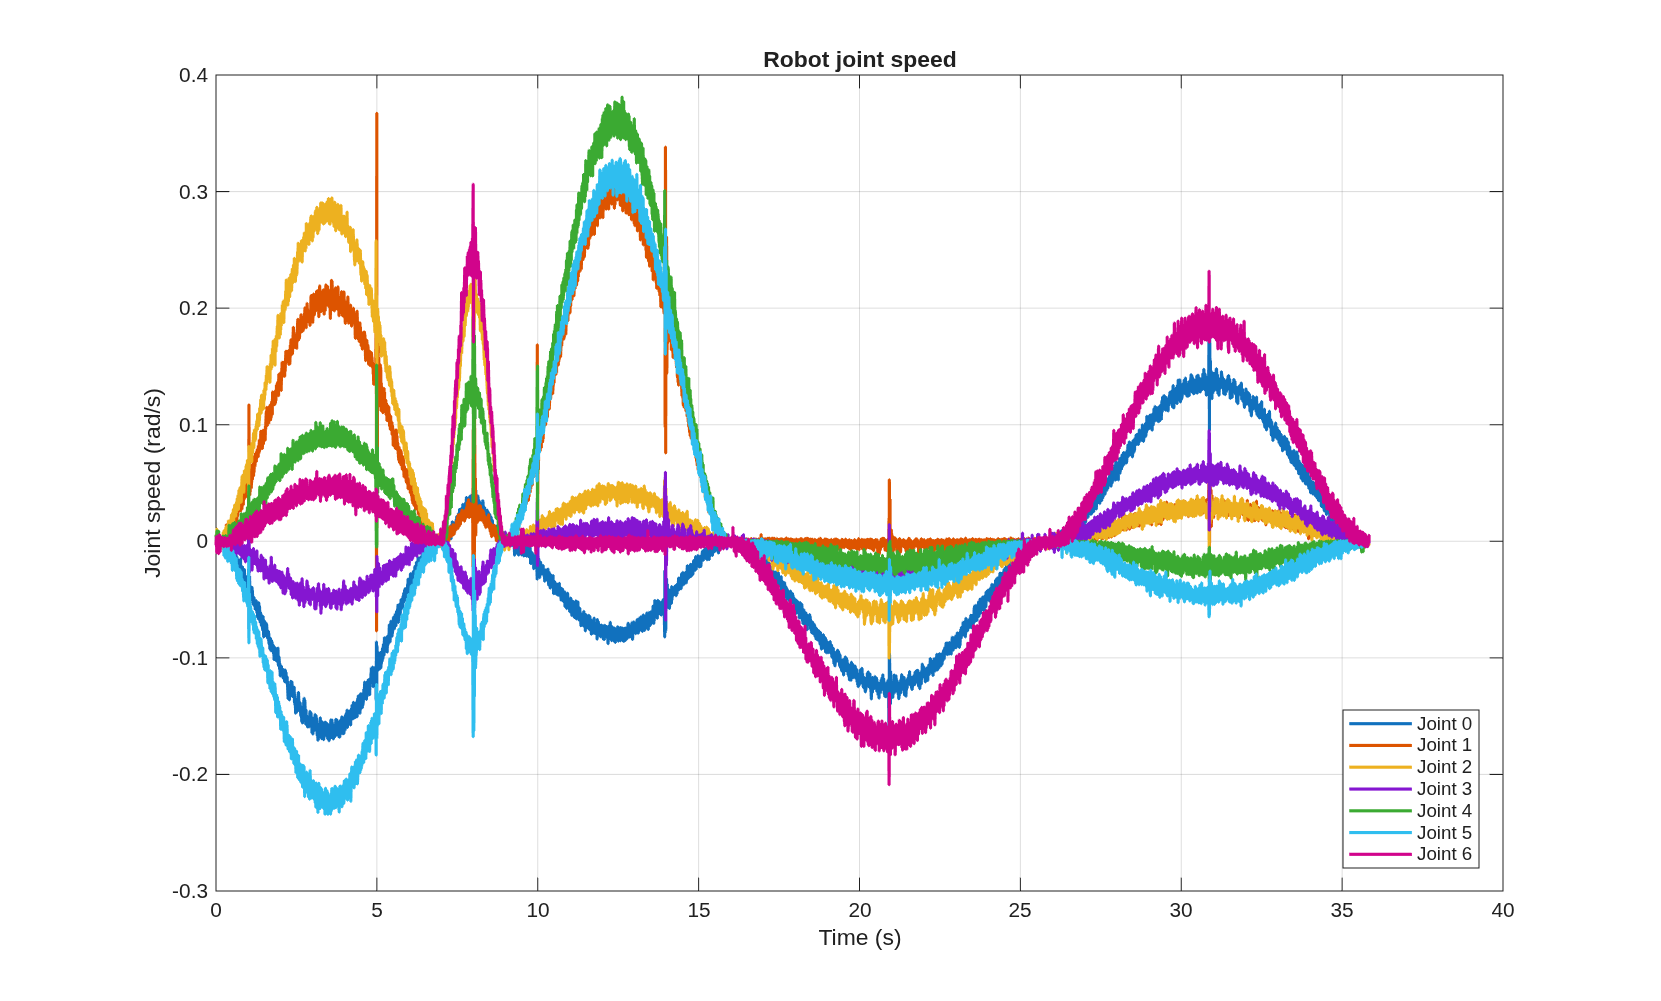
\includegraphics[width=0.85\linewidth]{figure_tesi/velocit_giunti_reale_PC}
	\caption{Profilo delle velocità ai giunti registrato con l'adozione del controllo di posizione. Si notino i picchi impulsivi e il fenomeno di \textit{jitter} dovuto alle discontinuità dei riferimenti.}
	\label{fig:velocitgiuntirealepc}
\end{figure}

\begin{figure}[htbp]
	\centering
	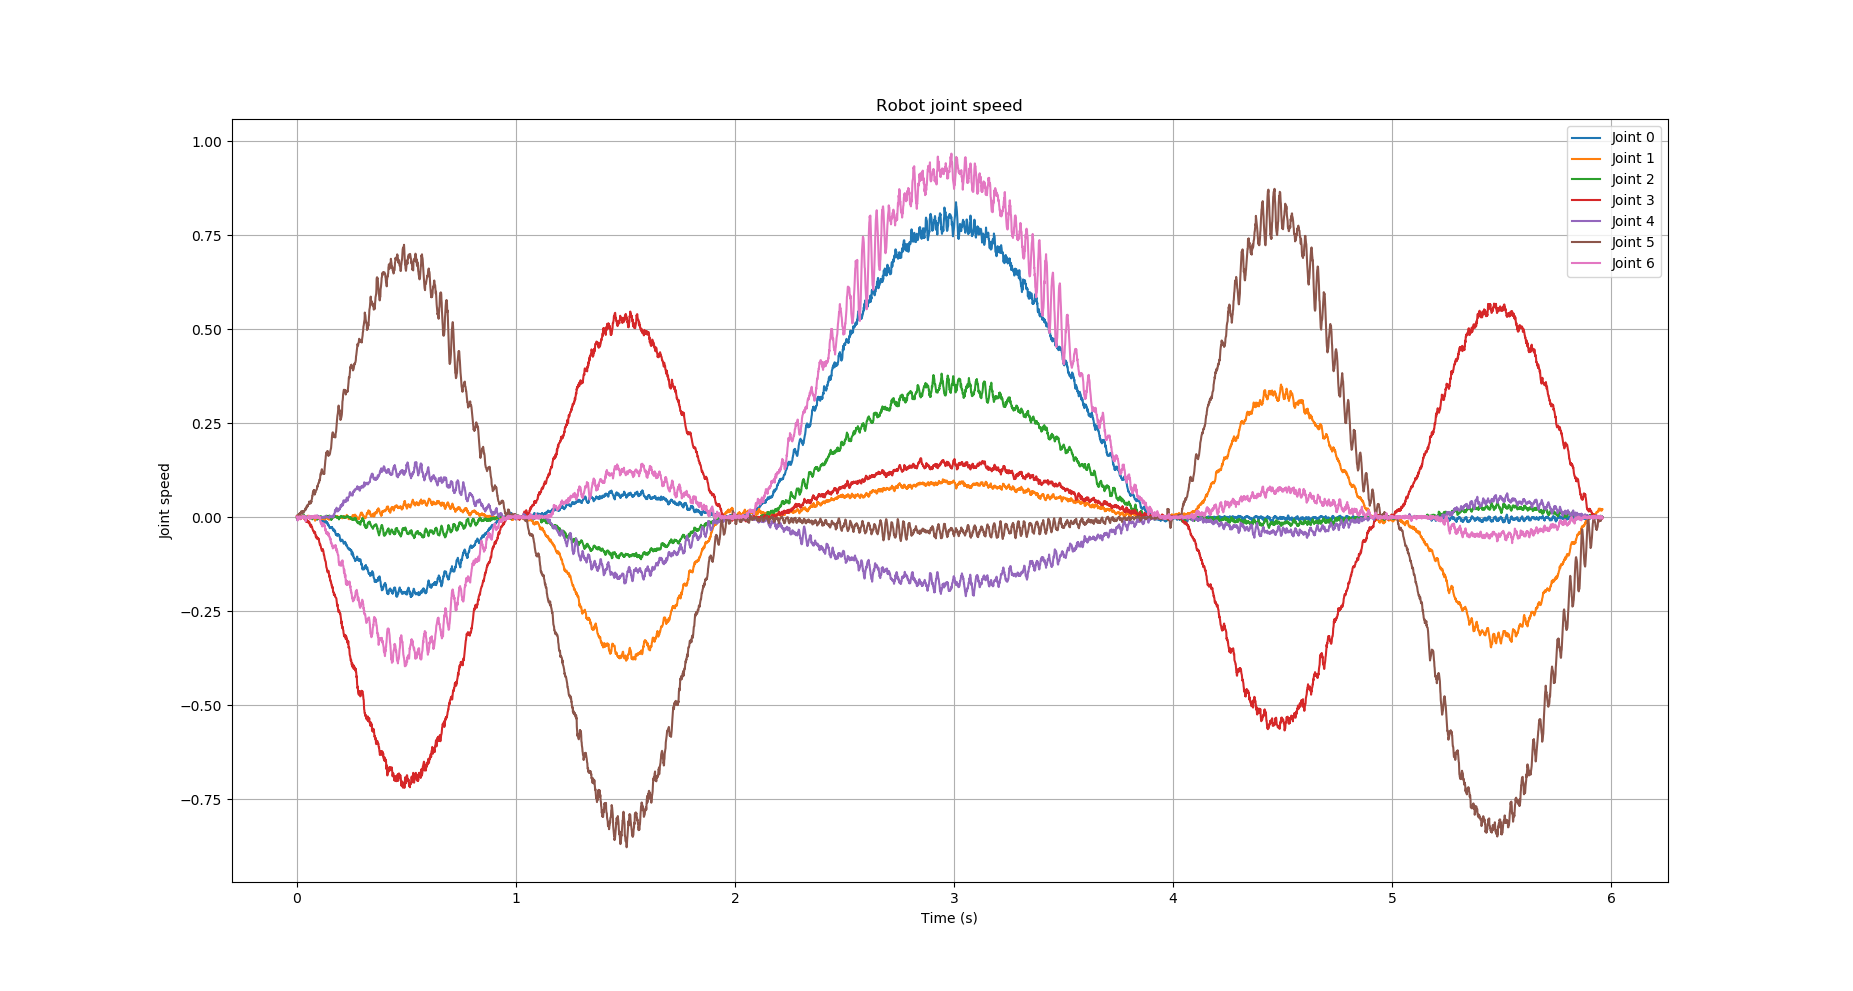
\includegraphics[width=0.85\linewidth]{figure_tesi/joint_speed_compensated_TC}
	\caption{Profilo delle velocità ai giunti con schema di controllo di coppia guidato dal regolatore PD. L'azione del controllore elimina i picchi, garantendo un'andamento fluido e privo di \textit{ripple}.}
	\label{fig:jointspeedcompensatedtc}
\end{figure}


\section{Risultati del primo approccio: arresto ottimizzato con capsule dinamiche}
\label{sec:risultati_primo_approccio}

Per valutare il comportamento del primo approccio di sicurezza, la metodologia è stata testata durante l'esecuzione di un compito nominale di \textit{pick-and-place}. Nel corso della traiettoria, al tempo $t \approx 2.5\text{ s}$, è stato introdotto un ostacolo virtuale mobile al fine di simulare un'intrusione nello spazio di lavoro e generare un evento di arresto di emergenza.

I risultati sperimentali, illustrati nelle Figure~\ref{fig:speedcalibrated1stoptc}, \ref{fig:duration1stoptc} e \ref{fig:raggicapsule1stoptc}, evidenziano i seguenti aspetti fondamentali:

\begin{itemize}
	\item \textbf{Profilo delle velocità ai giunti} (Figura~\ref{fig:speedcalibrated1stoptc}): alla ricezione del segnale di stop ($t \approx 2.5\text{ s}$), il controllore comanda una decelerazione fluida e continua, invertendo temporaneamente il verso del moto per riportare il robot verso la posizione iniziale in sicurezza, fino al completo azzeramento delle velocità di giunto.
	
	\item \textbf{Ottimizzazione online dei tempi di arresto} (Figura~\ref{fig:duration1stoptc}): la durata della frenata ottimizzata $T_{\text{stop}}$ viene ricalcolata continuamente in funzione dello stato cinematico istantaneo. In condizioni di velocità elevata, il valore stimato converge verso il limite superiore impostato ($0.4\text{ s}$), mentre al ridursi della velocità si attesta sul valore minimo di sicurezza ($0.25\text{ s}$).
	
	\item \textbf{Adattamento dinamico dei volumi delle capsule} (Figura~\ref{fig:raggicapsule1stoptc}): le dimensioni delle capsule di protezione si ridimensionano in tempo reale rispecchiando fedelmente il profilo del tempo di stop $T_{\text{stop}}$, espandendo il volume di inviluppo durante le fasi ad alta energia cinetica e riducendolo progressivamente durante la decelerazione.
\end{itemize}

Piccole asimmetrie o lievi sfasamenti temporali osservabili tra l'andamento delle velocità e le curve dei tempi di stop sono riconducibili all'architettura software multi-thread. Per garantire in modo deterministico la frequenza di aggiornamento di $1\text{ kHz}$ dell'anello di controllo di basso livello del manipolatore, l'algoritmo di ottimizzazione e il modulo di rilevamento degli ostacoli vengono eseguiti in modo asincrono su un thread dedicato a priorità distinta.

\begin{figure}[htbp]
	\centering
	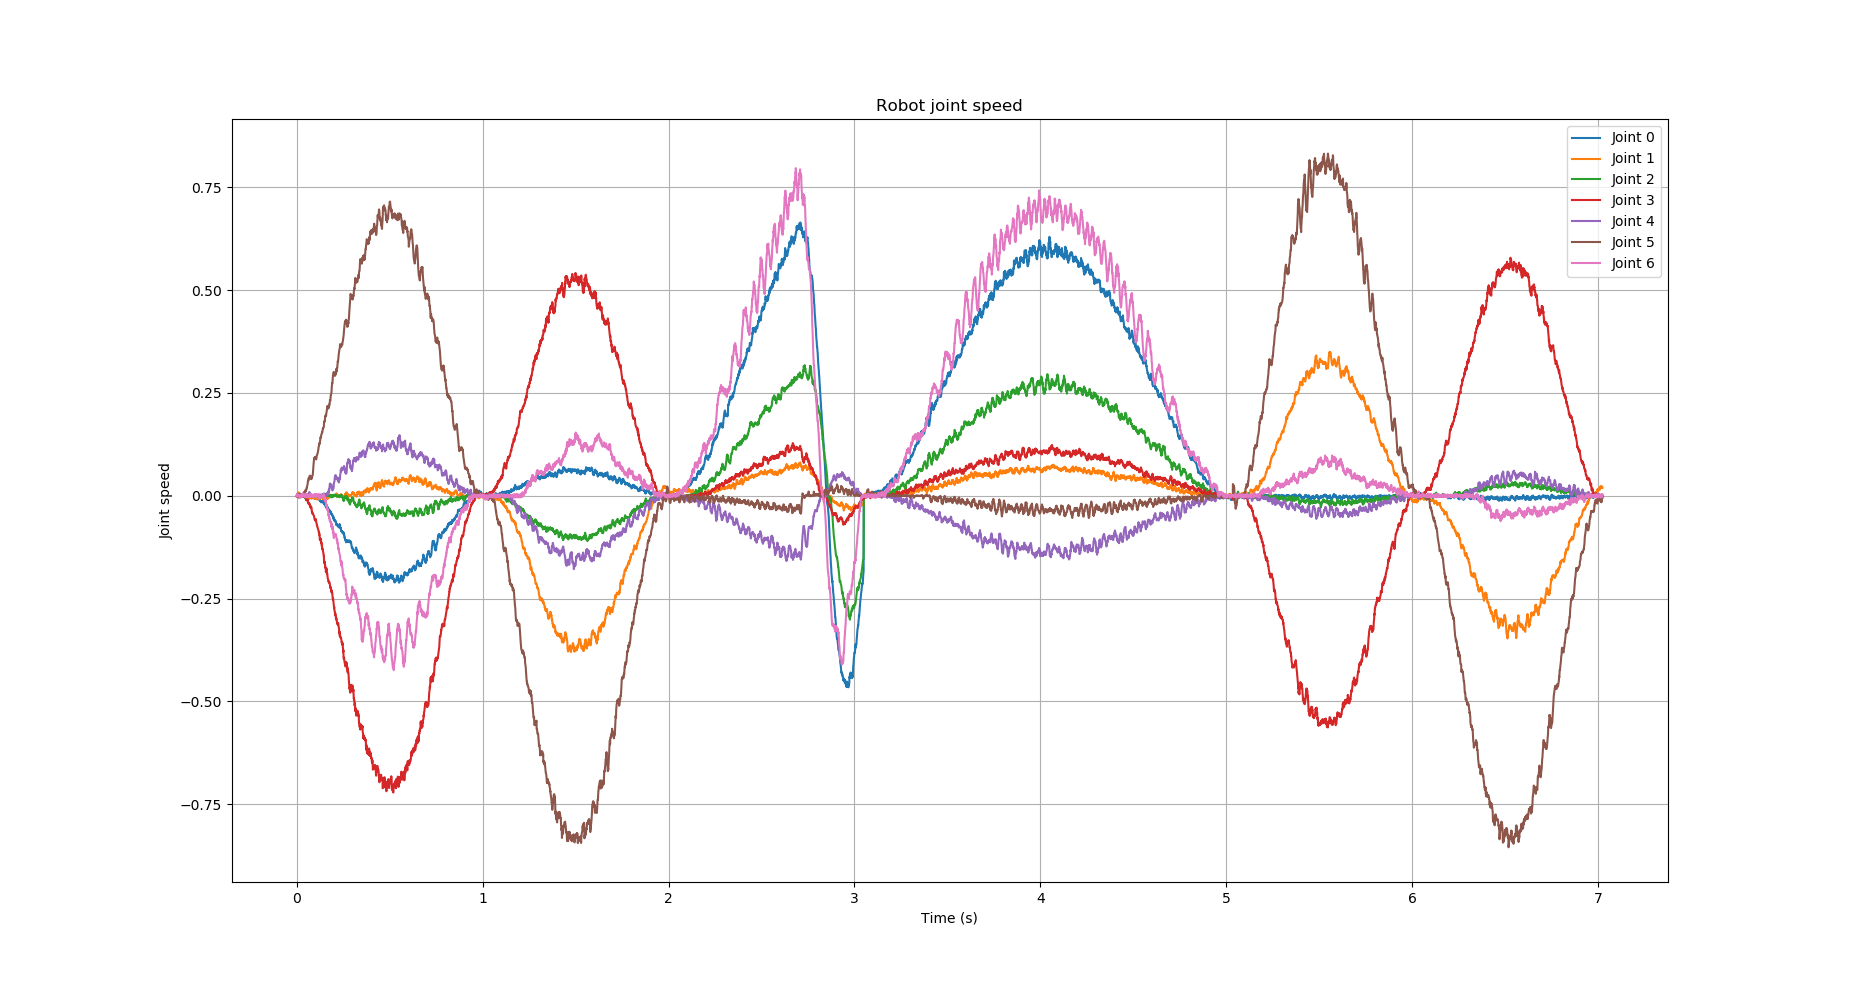
\includegraphics[width=0.85\linewidth]{figure_tesi/speed_calibrated_1stop_TC}
	\caption{Profilo temporale delle velocità ai giunti durante la traiettoria di \textit{pick-and-place}. Al tempo $t \approx 2.5\text{ s}$ viene rilevato l'ostacolo e attivata la procedura di arresto continuo.}
	\label{fig:speedcalibrated1stoptc}
\end{figure}

\begin{figure}[htbp]
	\centering
	
\includegraphics[width=0.85\linewidth]{figure_tesi/duration_1stop_TC}
	\caption{Andamento del tempo di arresto ottimizzato $T_{\text{stop}}$. Si nota la modulazione continua tra il valore minimo ($0.25\text{ s}$) e massimo ($0.4\text{ s}$) in base alla velocità istantanea.}
	\label{fig:duration1stoptc}
\end{figure}

\begin{figure}[htbp]
	\centering
	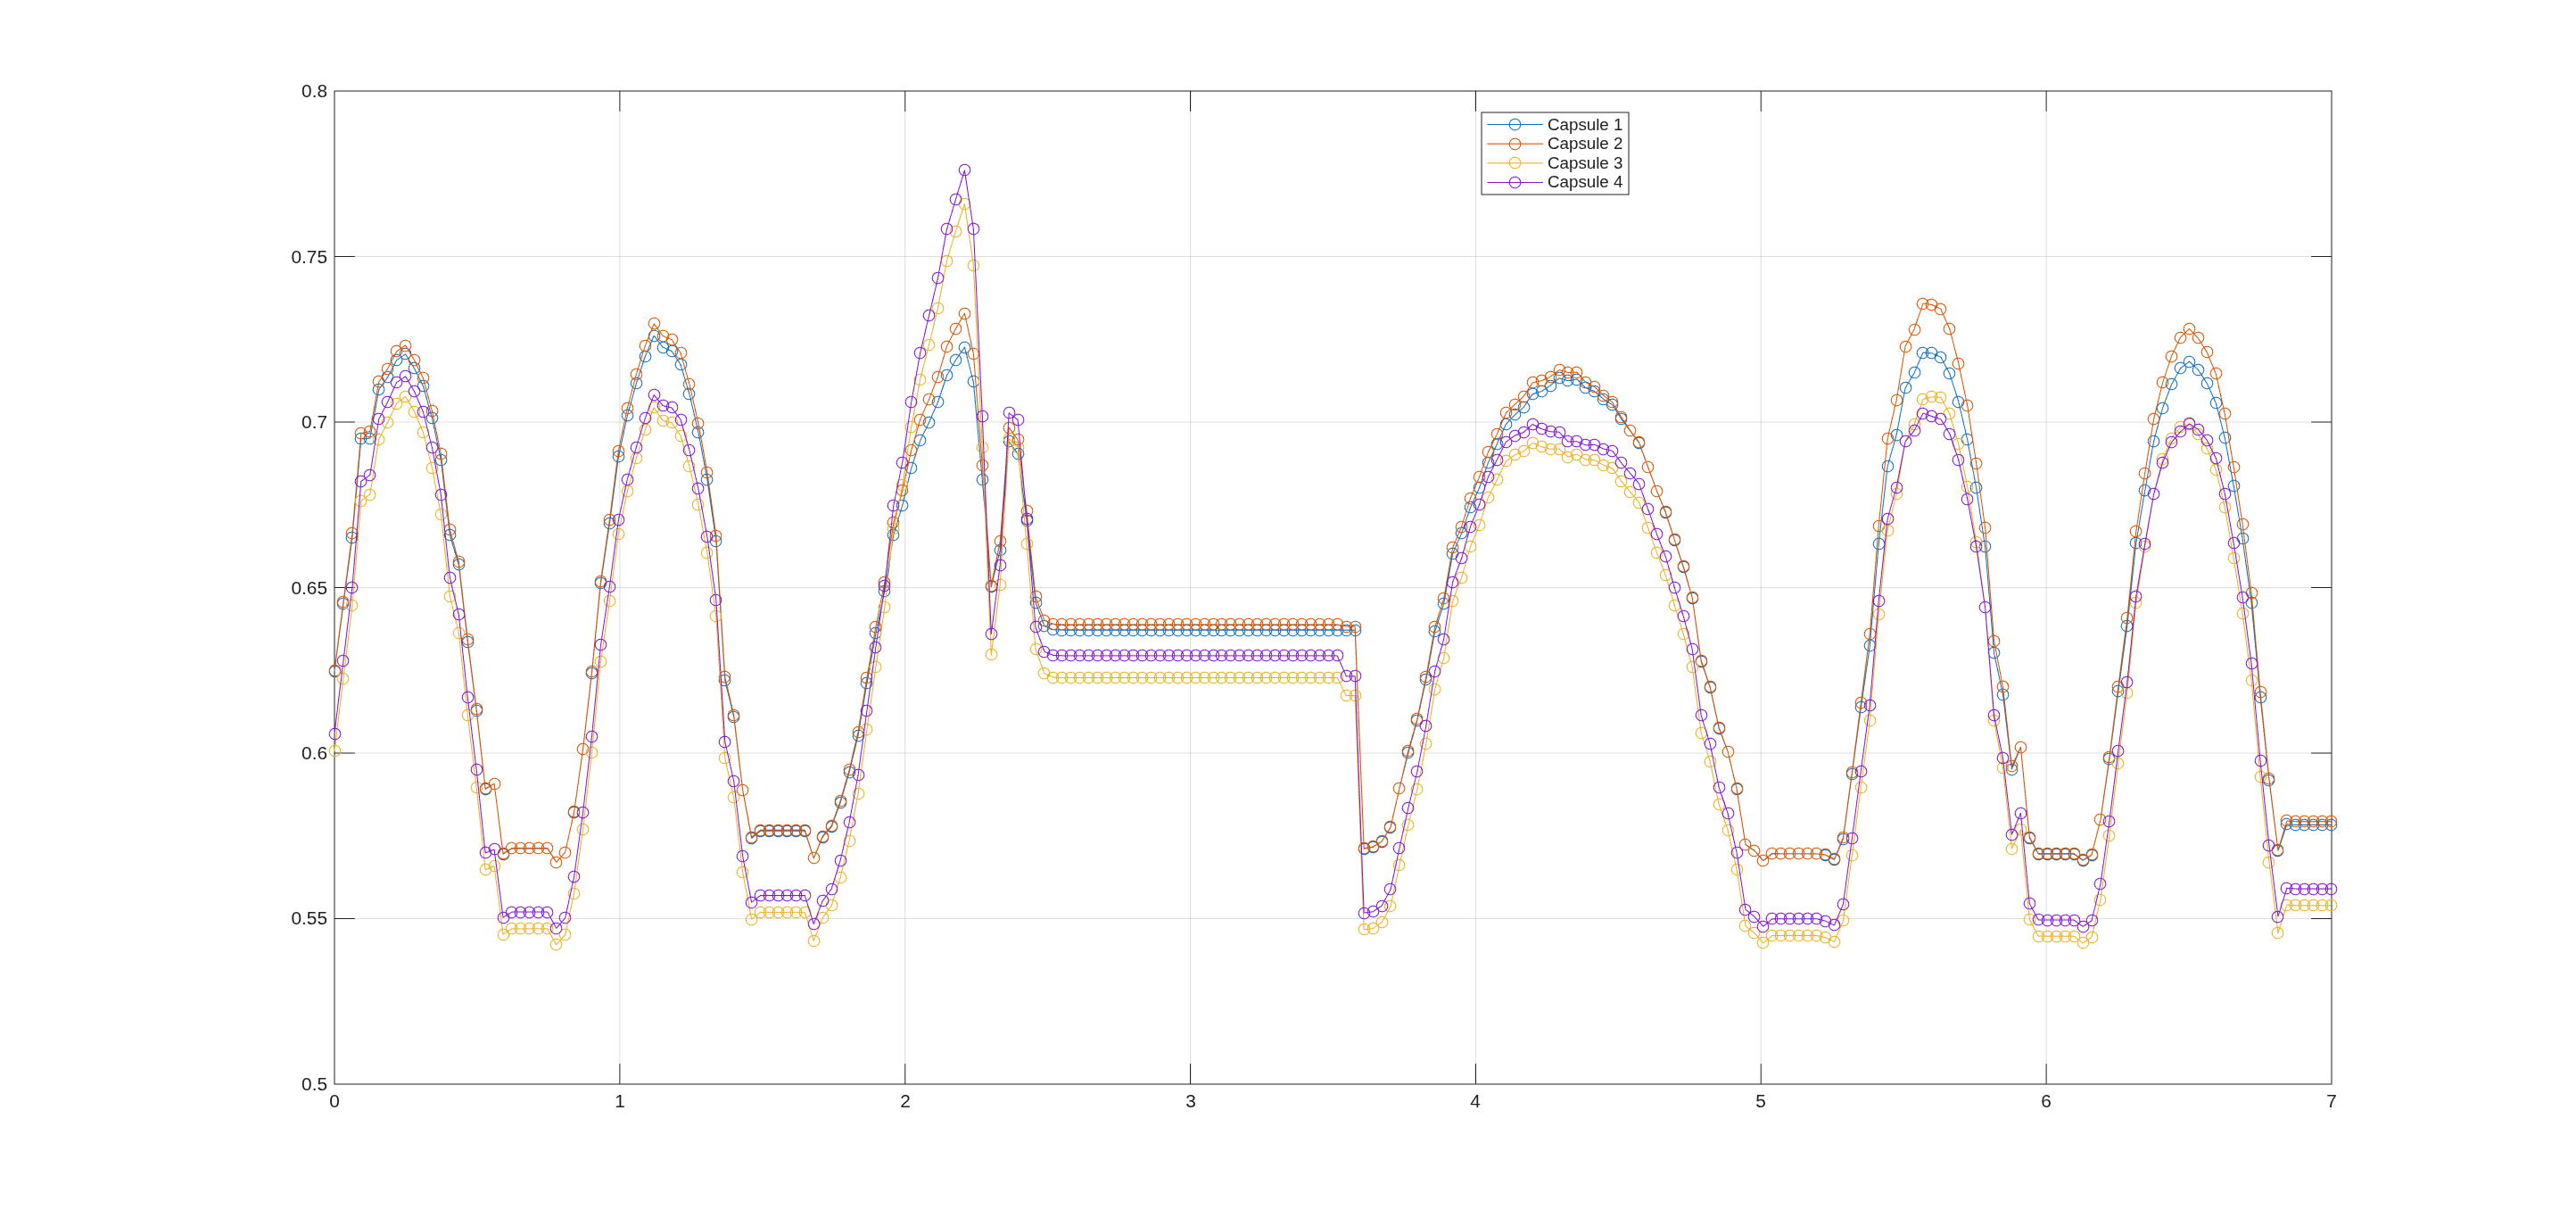
\includegraphics[width=0.85\linewidth]{figure_tesi/raggi_capsule_1stop_TC}
	\caption{Evoluzione temporale dei raggi delle capsule di protezione dinamiche, coerente con il profilo di decelerazione del robot.}
	\label{fig:raggicapsule1stoptc}
\end{figure}




\section{Secondo approccio}

\section{Contronto metriche di fluency}

\chapter{Conclusioni e sviluppi futuri}


sviluppi futuri: implementazione della predizione del moto dell'operatore (tipo con klt) per resistere a occlusioni

\bibliographystyle{unsrt}
\bibliography{bibliografia}

\end{document}
